\documentclass[preprint]{sigplanconf}

\usepackage{amssymb}
\usepackage{amsthm}
\usepackage{breakurl}             % Not needed if you use pdflatex only.
\usepackage{color}
\usepackage{epsfig}
\usepackage{esvect}
\usepackage{listings}
\usepackage{mathpartir}
\usepackage{MnSymbol}
\usepackage{multirow}
\usepackage{rotating}
\usepackage{paralist}

\newtheorem{definition}{Definition}
\newtheorem{theorem}{Theorem}
\newtheorem{lemma}{Lemma}
\newtheorem{proposition}{Proposition}
\newtheorem{corollary}{Corollary}

\setlength{\parskip}{0cm}
%\setlength{\parindent}{1em}

\DeclareMathOperator*{\argmin}{arg\,min}
\DeclareRobustCommand{\Cpp}{C\texttt{++}}
\DeclareRobustCommand{\code}[1]{{\lstinline[breaklines=false,escapechar=@]{#1}}}
\DeclareRobustCommand{\codebr}[1]{{\lstinline[breaklines=true]{#1}}}
\DeclareRobustCommand{\codehaskell}[1]{{\lstinline[breaklines=false,language=Haskell]{#1}}}
\DeclareRobustCommand{\codeocaml}[1]{{\lstinline[breaklines=false,language=Caml]{#1}}}
\DeclareRobustCommand{\concept}[1]{{\small\textsc{#1}}}

\newcommand{\exclude}[1]{}
\newcommand{\halfline}{\vspace{-1.5ex}}

%%%%%%%%%%%%%%%%%%%%%%%%%%%%%%%%%%%%%%%%%%%%%%%%%%%%%%%%%%%%%%%%%%%%%%%%%%%%%%
%%%%%%%%%%%%%%%%%%%%%%%%%%%%%%%%%%%%%%%%%%%%%%%%%%%%%%%%%%%%%%%%%%%%%%%%%%%%%%

% listings settings

%%%%%%%%%%%%%%%%%%%%%%%%%%%%%%%%%%%%%%%%%%%%%%%%%%%%%%%%%%%%%%%%%%%%%%%%%%%%%%
%%%%%%%%%%%%%%%%%%%%%%%%%%%%%%%%%%%%%%%%%%%%%%%%%%%%%%%%%%%%%%%%%%%%%%%%%%%%%%

\lstdefinestyle{C++}{language=C++,%
showstringspaces=false,
  columns=fullflexible,
  escapechar=@,
  basicstyle=\sffamily,
%  commentstyle=\rmfamily\itshape,
  moredelim=**[is][\color{white}]{~}{~},
  morekeywords={concept,decltype,noexcept,nullptr,requires},
  literate={[<]}{{\textless}}1      {[>]}{{\textgreater}}1 %
           {<}{{$\langle$}}1        {>}{{$\rangle$}}1 %
           {<=}{{$\leq$}}1          {>=}{{$\geq$}}1          
           {==}{{$==$}}2            {!=}{{$\neq$}}1 %
           {=>}{{$\Rightarrow\;$}}1 {->}{{$\rightarrow{}$}}1 %
           {<:}{{$\subtype{}\ $}}1  {<-}{{$\leftarrow$}}1 %
           {s1;}{{$s_1$;}}3 {s2;}{{$s_2$;}}3 {s3;}{{$s_3$;}}3 {s4;}{{$s_4$;}}3 {s5;}{{$s_5$;}}3 {s6;}{{$s_6$;}}3 {s7;}{{$s_7$;}}3 {sn;}{{$s_n$;}}3 {si;}{{$s_i$;}}3%
           {P1}{{$P_1$}}2 {P2}{{$P_2$}}2 {P3}{{$P_3$}}2 {P4}{{$P_4$}}2 {P5}{{$P_5$}}2 {P6}{{$P_6$}}2 {P7}{{$P_7$}}2 {Pn}{{$P_n$}}2 {Pi}{{$P_i$}}2%
           {D1}{{$D_1$}}2 {D2}{{$D_2$}}2 {D3}{{$D_3$}}2 {D4}{{$D_4$}}2 {D5}{{$D_5$}}2 {D6}{{$D_6$}}2 {D7}{{$D_7$}}2 {Dn}{{$D_n$}}2 {Di}{{$D_i$}}2%
           {T1}{{$T_1$}}2 {T2}{{$T_2$}}2 {T3}{{$T_3$}}2 {T4}{{$T_4$}}2 {T5}{{$T_5$}}2 {T6}{{$T_6$}}2 {T7}{{$T_7$}}2 {Tn}{{$T_n$}}2 {Ti}{{$T_i$}}2 {Tm}{{$T_m$}}2%
           {e1}{{$e_1$}}2 {e2}{{$e_2$}}2 {e3}{{$e_3$}}2 {e4}{{$e_4$}}2%
           {E1}{{$E_1$}}2 {E2}{{$E_2$}}2 {E3}{{$E_3$}}2 {E4}{{$E_4$}}2 {Ei}{{$E_i$}}2%
           {m_e1}{{$m\_e_1$}}4 {m_e2}{{$m\_e_2$}}4 {m_e3}{{$m\_e_3$}}4 {m_e4}{{$m\_e_4$}}4%
           {Divide}{{Divide}}6 {Either}{Either}6 %
           {Times}{{Times}}5 %
           {Match}{{\emph{Match}}}5 %
           {Case}{{\emph{Case}}}4 %
           {Qua}{{\emph{Qua}}}3 %
           {When}{{\emph{When}}}4 %
           {Otherwise}{{\emph{Otherwise}}}9 %
           {EndMatch}{{\emph{EndMatch}}}8 %
           {CM}{{\emph{CM}}}2 {KS}{{\emph{KS}}}2 {KV}{{\emph{KV}}}2 %
           {EuclideanDomain}{\concept{EuclideanDomain}}{15}  %
           {LazyExpression}{\concept{LazyExpression}}{14}    %
           {Polymorphic}{\concept{Polymorphic}}{11}          %
           {Convertible}{\concept{Convertible}}{11}          %
           {Integral}{\concept{Integral}}8                   %
           {SameType}{\concept{SameType}}8                   %
           {Pattern}{\concept{Pattern}}7                     %
           {Regular}{\concept{Regular}}7                     %
           {Object}{\concept{Object}}6                       %
           {Field}{\concept{Field}}5                         %
}
\lstset{style=C++}

\lstdefinestyle{Haskell}{language=Haskell,%
  morekeywords={out,view,real}
  literate={=>}{{$\Rightarrow\;$}}1 {->}{{$\rightarrow{}$}}1 {<-}{{$\leftarrow$}}1 {\\}{{$\lambda$}}1,
  moredelim=**[is][\color{red}]{`}{`},
  moredelim=**[is][\color{white}]{~}{~}
}

\lstdefinestyle{GJ}{language=Java,
  moredelim=**[is][\color{red}]{`}{`},
  moredelim=**[is][\color{white}]{~}{~}
}
\lstdefinestyle{Eiffel}{language=Eiffel,%
  literate={->}{{$\rightarrow$}}1,
  moredelim=**[is][\color{red}]{`}{`},
  moredelim=**[is][\color{white}]{~}{~}
}
\lstdefinestyle{Csharp}{language=[Sharp]C,
  morekeywords={where,require,type},
  literate={->}{{$\rightarrow{}$}}1,
  moredelim=**[is][\color{red}]{`}{`},
  moredelim=**[is][\color{white}]{~}{~}
}

\lstdefinestyle{ML}{language=ML,%
  literate={->}{{$\rightarrow{}$}}1,
  moredelim=**[is][\color{red}]{`}{`},
  moredelim=**[is][\color{white}]{~}{~}
}

\lstdefinestyle{Caml}{language=Caml,%
  morekeywords={when}
  literate={->}{{$\rightarrow{}$}}1,
  moredelim=**[is][\color{red}]{`}{`},
  moredelim=**[is][\color{white}]{~}{~}
}

%% grammar commands
\newcommand{\Rule}[1]{{\rmfamily\itshape{#1}}}
\newcommand{\Alt}{\ensuremath{|}}
\newcommand{\is}{$::=$}
\newcommand{\subtype}{\ensuremath{\texttt{\raisebox{-0.1ex}{<}\raisebox{0.05ex}{:}}}}
\newcommand{\subtypeD}{\ensuremath{<:_d}}
\newcommand{\lazyevals}{\Downarrow}
\newcommand{\evals}{\Rightarrow}
\newcommand{\evalspp}{\Rightarrow^+}
\newcommand{\DynCast}[2]{\ensuremath{\mathsf{dyn\_cast}\langle{#1}\rangle({#2})}}
\newcommand{\nullptr}{\ensuremath{\bot}}
\newcommand{\True}{\ensuremath{\mathsf{true}}}
\newcommand{\False}{\ensuremath{\mathsf{false}}}

\newcommand{\CWildcard}{\ensuremath{\mathit{\bf wildcard}}}
\newcommand{\CValue}   {\ensuremath{\mathit{\bf value}}}
\newcommand{\CVariable}{\ensuremath{\mathit{\bf variable}}}
\newcommand{\CExpr}    {\ensuremath{\mathit{\bf expr}}}
\newcommand{\CGuard}   {\ensuremath{\mathit{\bf guard}}}
\newcommand{\CCnstr}   {\ensuremath{\mathit{\bf ctor}}}

\newcommand{\Wildcard}   {\ensuremath{\CWildcard}}
\newcommand{\Value}[1]   {\ensuremath{\CValue\langle{#1}\rangle}}
\newcommand{\Variable}[1]{\ensuremath{\CVariable\langle{#1}\rangle}}
\newcommand{\ExprU}[2]   {\ensuremath{\CExpr\langle{#1},{#2}\rangle}}
\newcommand{\ExprB}[3]   {\ensuremath{\CExpr\langle{#1},{#2},{#3}\rangle}}
\newcommand{\ExprK}[3]   {\ensuremath{\CExpr\langle{#1},{#2},\cdots,{#3}\rangle}}
\newcommand{\Guard}[2]   {\ensuremath{\CGuard\langle{#1},{#2}\rangle}}
\newcommand{\Cnstr}[3]   {\ensuremath{\CCnstr\langle{#1},{#2},\cdots,{#3}\rangle}}

\newcommand{\f}[1]{{ {{#1\%}}}}
\newcommand{\s}[1]{{ {\bf \underline{#1\%}}}}
\newcommand{\n}[1]{{ {\bf ~ ~ ~ ~ }}}
\newcommand{\Opn}{{\scriptsize {\bf Open}}}
\newcommand{\Cls}{{\scriptsize {\bf Tag}}}
\newcommand{\Unn}{{\scriptsize {\bf Union}}}

%\newcommand{\gwNGPp}{\n{}}
%\newcommand{\gwNGKp}{\n{}}
 \newcommand{\gwNGUp}{\n{}}
%\newcommand{\gwNSPp}{\n{}}
%\newcommand{\gwNSKp}{\n{}}
 \newcommand{\gwNSUp}{\n{}}
%\newcommand{\vwNGPp}{\n{}}
%\newcommand{\vwNGKp}{\n{}}
 \newcommand{\vwNGUp}{\n{}}
%\newcommand{\vwNSPp}{\n{}}
%\newcommand{\vwNSKp}{\n{}}
 \newcommand{\vwNSUp}{\n{}}
%\newcommand{\vxNGPp}{\n{}}
%\newcommand{\vxNGKp}{\n{}}
 \newcommand{\vxNGUp}{\n{}}
%\newcommand{\vxNSPp}{\n{}}
%\newcommand{\vxNSKp}{\n{}}
 \newcommand{\vxNSUp}{\n{}}

%\newcommand{\gwNGPq}{\n{}}
%\newcommand{\gwNGKq}{\n{}}
 \newcommand{\gwNGUq}{\n{}}
%\newcommand{\gwNSPq}{\n{}}
%\newcommand{\gwNSKq}{\n{}}
 \newcommand{\gwNSUq}{\n{}}
%\newcommand{\vwNGPq}{\n{}}
%\newcommand{\vwNGKq}{\n{}}
 \newcommand{\vwNGUq}{\n{}}
%\newcommand{\vwNSPq}{\n{}}
%\newcommand{\vwNSKq}{\n{}}
 \newcommand{\vwNSUq}{\n{}}
%\newcommand{\vxNGPq}{\n{}}
%\newcommand{\vxNGKq}{\n{}}
 \newcommand{\vxNGUq}{\n{}}
%\newcommand{\vxNSPq}{\n{}}
%\newcommand{\vxNSKq}{\n{}}
 \newcommand{\vxNSUq}{\n{}}

%\newcommand{\gwNGPn}{\n{}}
%\newcommand{\gwNGKn}{\n{}}
 \newcommand{\gwNGUn}{\n{}}
%\newcommand{\gwNSPn}{\n{}}
%\newcommand{\gwNSKn}{\n{}}
 \newcommand{\gwNSUn}{\n{}}
%\newcommand{\vwNGPn}{\n{}}
%\newcommand{\vwNGKn}{\n{}}
 \newcommand{\vwNGUn}{\n{}}
%\newcommand{\vwNSPn}{\n{}}
%\newcommand{\vwNSKn}{\n{}}
 \newcommand{\vwNSUn}{\n{}}
%\newcommand{\vxNGPn}{\n{}}
%\newcommand{\vxNGKn}{\n{}}
 \newcommand{\vxNGUn}{\n{}}
%\newcommand{\vxNSPn}{\n{}}
%\newcommand{\vxNSKn}{\n{}}
 \newcommand{\vxNSUn}{\n{}}


%\newcommand{\gwYGPp}{\n{}}
% \newcommand{\gwYGKp}{\n{}}
 \newcommand{\gwYGUp}{\n{}}
%\newcommand{\gwYSPp}{\n{}}
% \newcommand{\gwYSKp}{\n{}}
 \newcommand{\gwYSUp}{\n{}}
%\newcommand{\vwYGPp}{\n{}}
% \newcommand{\vwYGKp}{\n{}}
 \newcommand{\vwYGUp}{\n{}}
%\newcommand{\vwYSPp}{\n{}}
% \newcommand{\vwYSKp}{\n{}}
 \newcommand{\vwYSUp}{\n{}}
%\newcommand{\vxYGPp}{\n{}}
% \newcommand{\vxYGKp}{\n{}}
 \newcommand{\vxYGUp}{\n{}}
%\newcommand{\vxYSPp}{\n{}}
% \newcommand{\vxYSKp}{\n{}}
 \newcommand{\vxYSUp}{\n{}}

%\newcommand{\gwYGPq}{\n{}}
% \newcommand{\gwYGKq}{\n{}}
 \newcommand{\gwYGUq}{\n{}}
%\newcommand{\gwYSPq}{\n{}}
% \newcommand{\gwYSKq}{\n{}}
 \newcommand{\gwYSUq}{\n{}}
%\newcommand{\vwYGPq}{\n{}}
% \newcommand{\vwYGKq}{\n{}}
 \newcommand{\vwYGUq}{\n{}}
%\newcommand{\vwYSPq}{\n{}}
% \newcommand{\vwYSKq}{\n{}}
 \newcommand{\vwYSUq}{\n{}}
%\newcommand{\vxYGPq}{\n{}}
% \newcommand{\vxYGKq}{\n{}}
 \newcommand{\vxYGUq}{\n{}}
%\newcommand{\vxYSPq}{\n{}}
% \newcommand{\vxYSKq}{\n{}}
 \newcommand{\vxYSUq}{\n{}}

%\newcommand{\gwYGPn}{\n{}}
% \newcommand{\gwYGKn}{\n{}}
 \newcommand{\gwYGUn}{\n{}}
%\newcommand{\gwYSPn}{\n{}}
% \newcommand{\gwYSKn}{\n{}}
 \newcommand{\gwYSUn}{\n{}}
%\newcommand{\vwYGPn}{\n{}}
% \newcommand{\vwYGKn}{\n{}}
 \newcommand{\vwYGUn}{\n{}}
%\newcommand{\vwYSPn}{\n{}}
% \newcommand{\vwYSKn}{\n{}}
 \newcommand{\vwYSUn}{\n{}}
%\newcommand{\vxYGPn}{\n{}}
% \newcommand{\vxYGKn}{\n{}}
 \newcommand{\vxYGUn}{\n{}}
%\newcommand{\vxYSPn}{\n{}}
% \newcommand{\vxYSKn}{\n{}}
 \newcommand{\vxYSUn}{\n{}}

 \newcommand{\GwNGPp}{\n{}}
 \newcommand{\GwNGKp}{\n{}}
 \newcommand{\GwNGUp}{\n{}}
 \newcommand{\GwNSPp}{\n{}}
 \newcommand{\GwNSKp}{\n{}}
 \newcommand{\GwNSUp}{\n{}}
%\newcommand{\VwNGPp}{\n{}}
%\newcommand{\VwNGKp}{\n{}}
 \newcommand{\VwNGUp}{\n{}}
%\newcommand{\VwNSPp}{\n{}}
%\newcommand{\VwNSKp}{\n{}}
 \newcommand{\VwNSUp}{\n{}}
%\newcommand{\VxNGPp}{\n{}}
%\newcommand{\VxNGKp}{\n{}}
 \newcommand{\VxNGUp}{\n{}}
%\newcommand{\VxNSPp}{\n{}}
%\newcommand{\VxNSKp}{\n{}}
 \newcommand{\VxNSUp}{\n{}}

 \newcommand{\GwNGPq}{\n{}}
 \newcommand{\GwNGKq}{\n{}}
 \newcommand{\GwNGUq}{\n{}}
 \newcommand{\GwNSPq}{\n{}}
 \newcommand{\GwNSKq}{\n{}}
 \newcommand{\GwNSUq}{\n{}}
%\newcommand{\VwNGPq}{\n{}}
%\newcommand{\VwNGKq}{\n{}}
 \newcommand{\VwNGUq}{\n{}}
%\newcommand{\VwNSPq}{\n{}}
%\newcommand{\VwNSKq}{\n{}}
 \newcommand{\VwNSUq}{\n{}}
%\newcommand{\VxNGPq}{\n{}}
%\newcommand{\VxNGKq}{\n{}}
 \newcommand{\VxNGUq}{\n{}}
%\newcommand{\VxNSPq}{\n{}}
%\newcommand{\VxNSKq}{\n{}}
 \newcommand{\VxNSUq}{\n{}}

 \newcommand{\GwNGPn}{\n{}}
 \newcommand{\GwNGKn}{\n{}}
 \newcommand{\GwNGUn}{\n{}}
 \newcommand{\GwNSPn}{\n{}}
 \newcommand{\GwNSKn}{\n{}}
 \newcommand{\GwNSUn}{\n{}}
%\newcommand{\VwNGPn}{\n{}}
%\newcommand{\VwNGKn}{\n{}}
 \newcommand{\VwNGUn}{\n{}}
%\newcommand{\VwNSPn}{\n{}}
%\newcommand{\VwNSKn}{\n{}}
 \newcommand{\VwNSUn}{\n{}}
%\newcommand{\VxNGPn}{\n{}}
%\newcommand{\VxNGKn}{\n{}}
 \newcommand{\VxNGUn}{\n{}}
%\newcommand{\VxNSPn}{\n{}}
%\newcommand{\VxNSKn}{\n{}}
 \newcommand{\VxNSUn}{\n{}}


 \newcommand{\GwYGPp}{\n{}}
 \newcommand{\GwYGKp}{\n{}}
 \newcommand{\GwYGUp}{\n{}}
 \newcommand{\GwYSPp}{\n{}}
 \newcommand{\GwYSKp}{\n{}}
 \newcommand{\GwYSUp}{\n{}}
%\newcommand{\VwYGPp}{\n{}}
% \newcommand{\VwYGKp}{\n{}}
 \newcommand{\VwYGUp}{\n{}}
%\newcommand{\VwYSPp}{\n{}}
% \newcommand{\VwYSKp}{\n{}}
 \newcommand{\VwYSUp}{\n{}}
%\newcommand{\VxYGPp}{\n{}}
% \newcommand{\VxYGKp}{\n{}}
 \newcommand{\VxYGUp}{\n{}}
%\newcommand{\VxYSPp}{\n{}}
% \newcommand{\VxYSKp}{\n{}}
 \newcommand{\VxYSUp}{\n{}}

 \newcommand{\GwYGPq}{\n{}}
 \newcommand{\GwYGKq}{\n{}}
 \newcommand{\GwYGUq}{\n{}}
 \newcommand{\GwYSPq}{\n{}}
 \newcommand{\GwYSKq}{\n{}}
 \newcommand{\GwYSUq}{\n{}}
%\newcommand{\VwYGPq}{\n{}}
% \newcommand{\VwYGKq}{\n{}}
 \newcommand{\VwYGUq}{\n{}}
%\newcommand{\VwYSPq}{\n{}}
% \newcommand{\VwYSKq}{\n{}}
 \newcommand{\VwYSUq}{\n{}}
%\newcommand{\VxYGPq}{\n{}}
% \newcommand{\VxYGKq}{\n{}}
 \newcommand{\VxYGUq}{\n{}}
%\newcommand{\VxYSPq}{\n{}}
% \newcommand{\VxYSKq}{\n{}}
 \newcommand{\VxYSUq}{\n{}}

 \newcommand{\GwYGPn}{\n{}}
 \newcommand{\GwYGKn}{\n{}}
 \newcommand{\GwYGUn}{\n{}}
 \newcommand{\GwYSPn}{\n{}}
 \newcommand{\GwYSKn}{\n{}}
 \newcommand{\GwYSUn}{\n{}}
%\newcommand{\VwYGPn}{\n{}}
% \newcommand{\VwYGKn}{\n{}}
 \newcommand{\VwYGUn}{\n{}}
%\newcommand{\VwYSPn}{\n{}}
% \newcommand{\VwYSKn}{\n{}}
 \newcommand{\VwYSUn}{\n{}}
%\newcommand{\VxYGPn}{\n{}}
% \newcommand{\VxYGKn}{\n{}}
 \newcommand{\VxYGUn}{\n{}}
%\newcommand{\VxYSPn}{\n{}}
% \newcommand{\VxYSKn}{\n{}}
 \newcommand{\VxYSUn}{\n{}}

% This file defines variables with performance numbers for the table in Evaluation section
% Data from 2011-08-30 
\newcommand{\vwYGKp}{\s{3}}
\newcommand{\vwYGKn}{\s{8}}
\newcommand{\vwYGKq}{\s{11}}
\newcommand{\vwYGPp}{\f{10}}
\newcommand{\vwYGPn}{\f{14}}
\newcommand{\vwYGPq}{\s{0}}
\newcommand{\vwYSKp}{\s{7}}
\newcommand{\vwYSKn}{\s{7}}
\newcommand{\vwYSKq}{\s{10}}
\newcommand{\vwYSPp}{\f{10}}
\newcommand{\vwYSPn}{\f{14}}
\newcommand{\vwYSPq}{\s{0}}
\newcommand{\vwNGKp}{\f{35}}
\newcommand{\vwNGKn}{\s{6}}
\newcommand{\vwNGKq}{\s{5}}
\newcommand{\vwNGPp}{\f{1}}
\newcommand{\vwNGPn}{\s{1}}
\newcommand{\vwNGPq}{\s{10}}
\newcommand{\vwNSKp}{\f{133}}
\newcommand{\vwNSKn}{\f{25}}
\newcommand{\vwNSKq}{\f{59}}
\newcommand{\vwNSPp}{\f{1}}
\newcommand{\vwNSPn}{\s{1}}
\newcommand{\vwNSPq}{\s{8}}

\newcommand{\vxYGKp}{\s{61}}
\newcommand{\vxYGKn}{\s{24}}
\newcommand{\vxYGKq}{\s{25}}
\newcommand{\vxYGPp}{\s{24}}
\newcommand{\vxYGPn}{\s{24}}
\newcommand{\vxYGPq}{\s{36}}
\newcommand{\vxYSKp}{\s{79}}
\newcommand{\vxYSKn}{\s{25}}
\newcommand{\vxYSKq}{\s{35}}
\newcommand{\vxYSPp}{\s{9}}
\newcommand{\vxYSPn}{\s{23}}
\newcommand{\vxYSPq}{\f{133}}
\newcommand{\vxNGKp}{\s{8}}
\newcommand{\vxNGKn}{\s{5}}
\newcommand{\vxNGKq}{\s{0}}
\newcommand{\vxNGPp}{\s{33}}
\newcommand{\vxNGPn}{\s{47}}
\newcommand{\vxNGPq}{\s{43}}
\newcommand{\vxNSKp}{\f{38}}
\newcommand{\vxNSKn}{\f{12}}
\newcommand{\vxNSKq}{\f{3}}
\newcommand{\vxNSPp}{\s{27}}
\newcommand{\vxNSPn}{\s{44}}
\newcommand{\vxNSPq}{\s{45}}

\newcommand{\gwYGKp}{\f{88}}
\newcommand{\gwYGKn}{\f{32}}
\newcommand{\gwYGKq}{\f{250}}
\newcommand{\gwYGPp}{\f{67}}
\newcommand{\gwYGPn}{\f{28}}
\newcommand{\gwYGPq}{\f{87}}
\newcommand{\gwYSKp}{\f{79}}
\newcommand{\gwYSKn}{\f{31}}
\newcommand{\gwYSKq}{\f{259}}
\newcommand{\gwYSPp}{\f{67}}
\newcommand{\gwYSPn}{\f{27}}
\newcommand{\gwYSPq}{\f{90}}
\newcommand{\gwNGKp}{\f{116}}
\newcommand{\gwNGKn}{\f{29}}
\newcommand{\gwNGKq}{\f{43}}
\newcommand{\gwNGPp}{\f{55}}
\newcommand{\gwNGPn}{\s{0}}
\newcommand{\gwNGPq}{\f{1}}
\newcommand{\gwNSKp}{\f{216}}
\newcommand{\gwNSKn}{\f{542}}
\newcommand{\gwNSKq}{\f{520}}
\newcommand{\gwNSPp}{\f{55}}
\newcommand{\gwNSPn}{\f{1}}
\newcommand{\gwNSPq}{\f{3}}

\newcommand{\VwYGKp}{\f{16}}
\newcommand{\VwYGKn}{\f{11}}
\newcommand{\VwYGKq}{\f{168}}
\newcommand{\VwYGPp}{\f{10}}
\newcommand{\VwYGPn}{\f{19}}
\newcommand{\VwYGPq}{\f{153}}
\newcommand{\VwYSKp}{\f{31}}
\newcommand{\VwYSKn}{\f{24}}
\newcommand{\VwYSKq}{\f{185}}
\newcommand{\VwYSPp}{\f{10}}
\newcommand{\VwYSPn}{\f{18}}
\newcommand{\VwYSPq}{\f{153}}
\newcommand{\VwNGKp}{\f{61}}
\newcommand{\VwNGKn}{\f{18}}
\newcommand{\VwNGKq}{\f{13}}
\newcommand{\VwNGPp}{\f{4}}
\newcommand{\VwNGPn}{\s{17}}
\newcommand{\VwNGPq}{\s{9}}
\newcommand{\VwNSKp}{\f{124}}
\newcommand{\VwNSKn}{\f{43}}
\newcommand{\VwNSKq}{\f{34}}
\newcommand{\VwNSPp}{\f{4}}
\newcommand{\VwNSPn}{\s{18}}
\newcommand{\VwNSPq}{\f{3}}
               
\newcommand{\VxYGKp}{\s{5}}
\newcommand{\VxYGKn}{\s{2}}
\newcommand{\VxYGKq}{\f{132}}
\newcommand{\VxYGPp}{\s{5}}
\newcommand{\VxYGPn}{\s{5}}
\newcommand{\VxYGPq}{\f{130}}
\newcommand{\VxYSKp}{\s{9}}
\newcommand{\VxYSKn}{\s{10}}
\newcommand{\VxYSKq}{\f{118}}
\newcommand{\VxYSPp}{\s{6}}
\newcommand{\VxYSPn}{\s{6}}
\newcommand{\VxYSPq}{\f{145}}
\newcommand{\VxNGKp}{\f{20}}
\newcommand{\VxNGKn}{\f{7}}
\newcommand{\VxNGKq}{\f{34}}
\newcommand{\VxNGPp}{\s{14}}
\newcommand{\VxNGPn}{\s{27}}
\newcommand{\VxNGPq}{\f{2}}
\newcommand{\VxNSKp}{\f{47}}
\newcommand{\VxNSKn}{\f{16}}
\newcommand{\VxNSKq}{\f{14}}
\newcommand{\VxNSPp}{\s{0}}
\newcommand{\VxNSPn}{\s{27}}
\newcommand{\VxNSPq}{\f{1}}

% This file defines variables with performance numbers for the table in Evaluation section
% Data from 2011-11-04 collected on Sierra for Linux under g++ (GCC) 4.4.5 20101112 (Red Hat 4.4.5-2)

\newcommand{\glYGKp}{\f{45}}
\newcommand{\glYGKn}{\f{82}}
\newcommand{\glYGKq}{\f{77}}
\newcommand{\glYGPp}{\f{36}}
\newcommand{\glYGPn}{\f{76}}
\newcommand{\glYGPq}{\f{53}}
\newcommand{\glYSKp}{\f{53}}
\newcommand{\glYSKn}{\f{88}}
\newcommand{\glYSKq}{\f{86}}
\newcommand{\glYSPp}{\f{33}}
\newcommand{\glYSPn}{\f{78}}
\newcommand{\glYSPq}{\f{55}}
\newcommand{\glNGKp}{\f{54}}
\newcommand{\glNGKn}{\f{97}}
\newcommand{\glNGKq}{\f{109}}
\newcommand{\glNGPp}{\f{19}}
\newcommand{\glNGPn}{\f{57}}
\newcommand{\glNGPq}{\f{62}}
\newcommand{\glNSKp}{\f{124}}
\newcommand{\glNSKn}{\f{603}}
\newcommand{\glNSKq}{\f{640}}
\newcommand{\glNSPp}{\f{16}}
\newcommand{\glNSPn}{\f{56}}
\newcommand{\glNSPq}{\f{56}}


\newsavebox{\sembox}
\newlength{\semwidth}
\newlength{\boxwidth}

\newcommand{\Sem}[1]{%
\sbox{\sembox}{\ensuremath{#1}}%
\settowidth{\semwidth}{\usebox{\sembox}}%
\sbox{\sembox}{\ensuremath{\left[\usebox{\sembox}\right]}}%
\settowidth{\boxwidth}{\usebox{\sembox}}%
\addtolength{\boxwidth}{-\semwidth}%
\left[\hspace{-0.3\boxwidth}%
\usebox{\sembox}%
\hspace{-0.3\boxwidth}\right]%
}

\newcommand{\authormodification}[2]{{\color{#1}#2}}
\newcommand{\ys}[1]{\authormodification{blue}{#1}}
\newcommand{\bs}[1]{\authormodification{red}{#1}}
\newcommand{\gdr}[1]{\authormodification{magenta}{#1}}

\begin{document}

%\conferenceinfo{DSL 2011}{Bordeaux, France} 
%\copyrightyear{2011} 
%\copyrightdata{[to be supplied]} 

\titlebanner{Technical Report}        % These are ignored unless
\preprintfooter{Y.Solodkyy, G.Dos Reis, B.Stroustrup: An Elegant and Efficient Pattern Matching Library for C++}   % 'preprint' option specified.

\title{An Elegant and Efficient Pattern Matching Library for C++}
%\subtitle{your \code{visit}, Jim, is not \code{accept}able anymore}
\subtitle{\code{accepting} aint no \code{visit}ors}

\authorinfo{Yuriy Solodkyy\and Gabriel Dos Reis\and Bjarne Stroustrup}
           {Texas A\&M University\\ Texas, USA}
           {\{yuriys,gdr,bs\}@cse.tamu.edu}

\maketitle

\begin{abstract}
Pattern matching is an abstraction mechanism that greatly simplifies code. We 
present functional-programming-style pattern matching for C++ 
implemented as a library. The library provides a uniform notation for 
matching against open hierarchy of run-time polymorphic classes as well as closed 
set of classes (including classes tagged by user and discriminated unions)
for which compile-time polymorphism can be used. The
 library integrates well with programming styles supported by C++, in 
particular it supports virtual and repeated multiple inheritance and can
 be used in generic code.

Our library equals or outperforms the visitor design pattern, as commonly 
used for pattern-matching scenarios in C++, and for many use cases it 
equals or outperforms equivalent code in languages with built-in pattern
 matching. Our solution better addresses more problems than the visitor
 design pattern does: it is non-intrusive and does not have 
extensibility restrictions. It also avoids control 
inversion and can be used in pattern-matching scenarios that visitors are ill suited for.
Code using patterns is significantly more concise and easier to comprehend than alternative solutions in C++.

Implementing pattern matching as a library allows us to experiment with syntax, 
implementation algorithms, and use while preserving benefit from the 
performance and portability provided by industrial compilers and support
 tools. The solution approach can be reused in other object-oriented 
languages to implement \emph{type switching}, \emph{type testing}, 
\emph{pattern matching} and \emph{multiple dispatch} efficiently.

The library was motivated by and is used for applications involving large, typed, abstract syntax trees.
\end{abstract}

\category{D}{1}{5}
\category{D}{3}{3}

\terms
Languages, Design

\keywords
Pattern Matching, Type Switch, Typecase, Visitor Design Pattern, Expression Problem, Memoization, C++

\section{Introduction} %%%%%%%%%%%%%%%%%%%%%%%%%%%%%%%%%%%%%%%%%%%%%%%%%%%%%%%%%
\label{sec:intro}

%Conventional object-oriented programming practice suggests \emph{Visitor Design 
%Pattern}~\cite{DesignPatterns} for principled traversal of structured data such 
%as those manipulated by compilers, GUI frameworks, etc. However, our experience 
%with various \Cpp{} front-ends and program analysis frameworks~\cite{Pivot09,Phoenix,Clang} 
%have been rather unsatisfactory. We found visitors unsuitable to express our 
%application logic, surprisingly hard to teach students, and slow. We found 
%dynamic casts in many places, often nested. This suggested that users preferred 
%shorter, cleaner, and more direct codes to visitors, even at the high cost in 
%performance. Most of the dynamic cast usage mimicked the moral equivalent of 
%pattern matching as found in modern functional programming languages.

Pattern matching is an abstraction mechanism popularized by the functional
programming community, most notably ML~\cite{ML78}, Hope~\cite{BMS80}, 
Miranda~\cite{Miranda85}, OCaml~\cite{OPM01} and Haskell~\cite{haskell90},
and recently adopted by several multi-paradigm and object-oriented programming 
languages such as Scala~\cite{Scala2nd}, F\#~\cite{Syme07}, 
Newspeak~\cite{geller2010pattern}, Fortress~\cite{RPS10}, 
Thorn~\cite{Thorn2012}, Grace~\cite{Grace2012}, and dialects of 
\Cpp{}\cite{Prop96,App}, Eiffel~\cite{Moreau:2003} and 
Java~\cite{Odersky97pizzainto,Liu03jmatch:iterable,HydroJ2003,OOMatch07thesis,padl08}.
It provides syntax very close to mathematical notation and allows the user to 
describe tersely a (possibly infinite) set of values accepted by the pattern. 
A \emph{pattern} is an immediate predicate on an implicit argument that can be 
used to check properties and bind parameters inherent to them. The pattern is 
usually more specialized and thus more concise, expressive and readable than 
equivalent imperative code, even when the latter is expressed with unnamed 
$\lambda$-expressions. Patterns are similar to $\lambda$-expressions, however, in 
that they are rarely repeated in several places in code, which makes them 
unattractive for code reuse through a dedicated predicate. The difference 
between patterns and $\lambda$-expressions lies in the brevity of code, their 
composition and interaction.

Expressivity of pattern matching has been considered so crucial in certain application domains, 
that it became the number one reason for choosing a functional language for the 
job in those domains. In their experience report on implementing Frama-C static 
analyzer, Cuoq et al~\cite{FramaC09} list expressiveness as the number one reasons for using 
OCaml instead of \Cpp{}. Similar sentiments are expressed in 
two other experience reports detailing implementation of a high-performance 
trading platform in OCaml~\cite{Minsky08} and implementation of a hardware-design 
toolset in Haskell~\cite{Nanavati08}.

We thus consider how functional-style pattern matching can be added to \Cpp{}.
Introduction of pattern matching into a new language is nontrivial;
introducing it into an existing language in widespread use is an even greater 
challenge. The obvious utility of the feature is easily compromised by the need 
to fit into the language's syntax, semantics, and tool chains. A prototype 
implementation requires more effort than for an experimental language.
It is also
harder to get into use because mainstream users are unwilling to try 
non-portable, non-standard, and unoptimized features, so we need to provide an optimized implementation. 
To balance utility and effort we took the Semantically Enhanced Library Language 
(SELL) approach~\cite{SELL,BSGDR05} that advocates for extending a general-purpose 
programming language with a library, aided by a tool. With pattern matching, we 
(somewhat surprisingly) managed to avoid external tool support by relying on 
some pretty nasty macro hacking and template meta-programming to provide a 
conventional and convenient interface to an efficient library implementation.

%Before we go 
%any further, though, we need to explicitly clarify one aspect. Throughout the 
%paper, when not stated otherwise, by pattern matching we mean run-time pattern 
%matching -- a facility that can be used to analyze and decompose run-time values.
%This is important, because \Cpp{} has a pure functional sublanguage in it with 
%striking similarity to ML and Haskell that has a very extensive compile-time 
%pattern-matching facility in it~\cite{Milewski11}. The sublanguage in question 
%is the template facilities of \Cpp{}, which allows one to encode computations at
%compile time, and has been shown to be Turing complete\cite{veldhuizen:templates_turing_complete}. 
%The key observation in the analogy to pattern matching is that partial and 
%explicit template specialization of \Cpp{} class templates are similar to 
%defining equations for Haskell functions. It is also used in \Cpp{} for similar 
%purposes: case analysis over families of types, structural decomposition of 
%types, overload resolution etc. It turns out we can use this compile-time 
%pattern matching facility to build a very expressive, efficient and extensible 
%run-time pattern matching solution.

%By efficient, we mean about as fast as functional languages for closed cases and
%much better than code generated for visitor patterns by commercial optimizers 
%for open cases\cite{TypeSwitch}.

\subsection{Summary}

We present a functional-style pattern matching for \Cpp{} built as an ISO 
\Cpp{}11 library. Our solution:

\begin{compactitem}
\setlength{\itemsep}{0pt}
\setlength{\parskip}{0pt}
  \item Makes patterns first-class citizens in the language (\textsection\ref{sec:pat}).
  \item Is open to introduction of new patterns into the library.
  \item Is type safe. Inappropriate applications of patterns to subjects are manifested as compile-time errors.  
  \item Is non-intrusive and can be retroactively applied to existing types (\textsection\ref{sec:bnd}).
%  \item Provides a unified syntax for various encodings of extensible 
%        hierarchical datatypes in \Cpp{} (\textsection\ref{sec:unisyn}).
  \item Provides an alternative view on the controversial n+k patterns, which 
        leaves the choice of semantics to the user and makes them similar to 
        constructor patterns (\textsection\ref{sec:slv}).
  \item Supports a limited form of views (\textsection\ref{sec:view}).
  \item Generalizes open type switch to multiple scrutinies and enables patterns 
        in case clauses (\textsection\ref{sec:matchstmt}).
%  \item Is simpler than conventional object-oriented or union-based alternatives.
%  \item Improves performance compared to alternatives in real applications~\cite{TypeSwitch}.
  \item Demonstrates that compile-time composition of patterns through 
        concepts is superior to run-time composition of patterns through 
        polymorphic interfaces in terms of performance, expressiveness and 
        static type checking (\textsection\ref{sec:patcmp}).
\end{compactitem}

%The library in this respect is nothing else than a set of \Cpp{} concepts 
%guiding the composition of patterns combined with a set of macros providing a 
%suitable surface syntax. 

%We observe that the approach we use for open type switching generalizes easily 
%to the case of multiple scrutinies (subjects), while the closed approach does 
%not.

\noindent
Our library sets a minimum for performance, extensibility, brevity, 
clarity and usefulness of any language solution for pattern matching 
in \Cpp{}. It provides full functionality, so we can experiment with the use of 
pattern matching in \Cpp{} and compare it to existing language alternatives.
Our solution can be used today given 
current support of \Cpp{}11 (e.g., GCC and Microsoft \Cpp{}) without any 
additional tool support.

The rest of the paper is structured as following. Section~\ref{sec:cpppat} 
introduces common terminology and demonstrates the syntax enabled by the 
\emph{Mach7} library~\cite{TS12}. Section~\ref{sec:impl} provides some 
implementation details that make our extension possible. Section~\ref{sec:eval} 
compares our solution to some alternatives. Section~\ref{sec:rw} discusses 
related work, while Section~\ref{sec:cc} concludes by discussing some future 
directions and possible improvements. Appendix~\ref{sec:prelim} provides some 
details about \Cpp{} concepts and the syntax used in the paper.

\section{Background} %%%%%%%%%%%%%%%%%%%%%%%%%%%%%%%%%%%%%%%%%%%%%%%%%%%%%%%%%%%
\label{sec:bg}

Pattern matching in the context of a programming language was first introduced 
in a string manipulation language SNOBOL\cite{SNOBOL64}. Its fourth 
reincarnation SNOBOL4 had patterns as first-class data types providing 
operations of concatenation and alternation on them\cite{SNOBOL71}. The first 
reference to a pattern-matching construct that resembles the one found in 
statically typed functional languages today is usually attributed to Burstall 
and his work on structural induction\cite{Burstall69provingproperties}.

In the context of object-oriented programming, pattern matching has been first 
explored in Pizza programming language\cite{Odersky97pizzainto}. These efforts 
have been continued in Scala\cite{Scala2nd} and together with notable work of 
Burak Emir on \emph{Object-Oriented Pattern Matching}\cite{EmirThesis} have 
resulted in incorporation of pattern matching into the language.

%The first tree based pattern matching methods were found in Fred McBride's 
%extension of LISP in 1970.

%ML and Haskell further popularized pattern matching ...

Pattern matching has been closely related to \emph{algebraic data types} and 
\emph{equational reasoning} since the early days of functional programming.
In languages like ML and Haskel an \emph{Algebraic Data Type} is a data type 
each of whose values is picked from a disjoint sum of (possibly recursive) data 
types, called \emph{variants}. Each of the variants is marked with a unique 
symbolic constant called \emph{constructor}, while the set of all constructors 
of a given type is called \emph{signature}. Constructors provide a convenient 
way of creating a value of its variant type as well as a way of discriminating 
its variant type from the algebraic data type through pattern matching.

Algebraic data type \codeocaml{expr} from Section~\ref{sec:intro} consists of 5 
variants, marked with constructors \codeocaml{Value}, \codeocaml{Plus}, 
\codeocaml{Minus}, \codeocaml{Times} and \codeocaml{Divide} respectively. 
Constructor \codeocaml{Value} expects a value of type \codeocaml{int} during 
construction, as well as any pattern that admits values of type \codeocaml{int} 
during decomposition through pattern matching. Similarly, the other four 
constructors expect a value of a cartesian product of two \codeocaml{expr} 
types during construction, as well as any pattern that would admit a value of 
such type during decomposition.

Algebraic data types can be parameterized and recursive, as demonstrated by the 
following Haskell code that defines a binary tree parameterized on type 
\codehaskell{k} of keys and type \codehaskell{d} of data stored in the nodes:

\begin{lstlisting}[language=Haskell]
data Tree k d = Node k d (Tree k d) (Tree k d) | Leaf
\end{lstlisting}

\noindent
Naturally, they can be decomposed in a generic algorithm like the function 
\code{find} below, defined through case analysis on the tree's structure:

\begin{lstlisting}[language=Haskell]
find :: (Ord k) => k -> Tree k d -> Maybe d
find i Leaf = Nothing
find i (Node key item left right) = 
    if i == key 
    then Just item 
    else 
        if i [<] key 
        then find i left 
        else find i right
\end{lstlisting}

\noindent
The set of values described by such an algebraic data type is defined 
inductively as the least set closed under constructor functions of its variants.
Algebraic data types draw their name from the practice of using case distinction 
in mathematical function definitions and proofs that involve \emph{algebraic 
terms}.

One of the main differences of algebraic data types from classes in 
object-oriented languages is that an algebraic data type definition is 
\emph{closed} because it fixes the structure of its instances once and for all. 
Once we have listed all the variants a given algebraic data type may have we 
cannot extend it with new variants without modifying its definition. This is not 
the case in object-oriented languages, where classes are \emph{open} to 
extension through subclassing. Notable exceptions to this restriction in 
functional community are \emph{polymorphic variants} in OCaml\cite{garrigue-98} 
and \emph{open data types} in Haskell\cite{LohHinze2006}, which allow addition 
of new variants later. These extensions, however, are simpler than object-oriented 
extensions as neither polymorphic variants nor open data types form subtyping 
relation between themselves: open data types do not introduce any subtyping 
relation, while the subtyping relation on polymorphic variants is a 
\emph{semantic subtyping} similar to that of XDuce\cite{HosoyaPierce2000}, which 
is based on the subset relation between values of the type. In either case they 
maintain the important property that each value of the underlying algebraic data 
type belongs to exactly one disjoint subset tagged with a constructor. The 
\emph{nominative subtyping} of object-oriented languages does not usually have 
this disjointness making classes effectively have multiple types. In particular, 
the case of disjoint constructors can be seen as a degenerated case of a flat 
class hierarchy among the multitude of possible class hierarchies.

Closedness of algebraic data types is particularly useful for reasoning about 
programs by case analysis and allows the compiler to perform an automatic 
\emph{incompleteness} check -- test of whether a given \emph{match statement} 
covers all possible cases. Similar reasoning about programs involving extensible 
data types is more involved as we are dealing with potentially open set of 
variants. \emph{Completeness} check in such scenario reduces to checking presence 
of a case that handles the static type of the subject. Absence of such a case,
however, does not necessarily imply incompleteness, only potential incompleteness, 
as the answer will depend on the actual set of variants available at run-time.

A related notion of \emph{redundancy} checking arises from the 
tradition of using \emph{first-fit} strategy in pattern matching. It warns the 
user of any \emph{case clause} inside a match statement that will 
never be entered because of a preceding one being more general. Object-oriented 
languages, especially C++, typically prefer \emph{best-fit} strategy (e.g. for 
overload resolution and class template specialization) because it is not prone 
to errors where semantics of a statement might change depending on the ordering 
of preceding definitions. The notable exception in C++ semantics that prefers 
the \emph{first-fit} strategy is ordering of \code{catch} handlers of a 
\code{try}-block. Similarly to functional languages the C++ compiler will perform 
\emph{redundancy} checking on catch handlers and issue a warning that lists the 
redundant cases. We use this property of the C++ type system to perform redundancy 
checking of our match statements in \textsection\ref{sec:redun}.

The patterns that work with algebraic data types we have seen so far are 
generally called \emph{tree patterns} or \emph{constructor patterns}. Their 
analog in object-oriented languages is often referred to as \emph{type pattern} 
since it may involve type testing and type casting. Special cases of these patterns 
are \emph{list patterns} and \emph{tuple patterns}. The former lets one split a 
list into a sequence of elements in its beginning and a tail with the help of 
list constructor \codehaskell{:} and an empty list constructor \codehaskell{[]} 
e.g. \codehaskell{[x:y:rest]}. The latter does the same with tuples using tuple
constructor \codehaskell{(,,...,)} e.g. \codehaskell{([x:xs],'b',(1,2.0),"hi",True)}.

Pattern matching is not used solely with algebraic data types and can equally 
well be applied to built-in types. The following Haskell code defines factorial 
function in the form of equations:

\begin{lstlisting}[language=Haskell]
factorial 0 = 1
factorial n = n * factorial (n-1)
\end{lstlisting}

\noindent
Here 0 in the left hand side of the first \emph{equation} is an example of a 
\emph{value pattern} (also known as \emph{constant pattern}) that will only 
match when the actual argument passed to the function factorial is 0. The 
\emph{variable pattern} \codehaskell{n} (also referred to as \emph{identifier 
pattern}) in the left hand side of the second equation will match any value, 
\emph{binding} variable \codehaskell{n} to that value in the right hand side of 
equation. Similarly to variable pattern, the \emph{wildcard pattern} \codehaskell{_} 
will match any value, neither binding it to a variable nor even obtaining it. 
Value patterns, variable patterns and wildcard patterns are  
generally called \emph{primitive patterns}. Patterns like variable and wildcard 
patterns that never fail to match are called \emph{irrefutable}, in contrast to 
\emph{refutable} patterns like value patterns, which may fail to match.

In Haskell 98\cite{Haskell98Book} the above definition of factorial could also 
be written as:

\begin{lstlisting}[language=Haskell]
factorial 0 = 1
factorial (n+1) = (n+1) * factorial n
\end{lstlisting}

\noindent
The \codehaskell{(n+1)} pattern in the left hand side of equation is an example of 
\emph{n+k pattern}. According to its informal semantics ``Matching an $n+k$ 
pattern (where $n$ is a variable and $k$ is a positive integer literal) against 
a value $v$ succeeds if $v \ge k$, resulting in the binding of $n$ to $v-k$, and 
fails otherwise''\cite{haskell98}. n+k patterns were introduced into Haskell to 
let users express inductive functions on natural numbers in much the same way as 
functions defined through case analysis on algebraic data types. Besides 
succinct notation, such language feature could facilitate automatic proof of 
termination of such functions by compiler. Peano numbers, used as an analogy to 
algebraic data type representation of natural numbers, is not always the best 
abstraction for representing other mathematical operations however. This,  
together with numerous ways of defining semantics of generalized n+k patterns 
were some of the reasons why the feature was never generalized in Haskell to 
other kinds of expressions, even though there were plenty of known applications. 
Moreover, numerous debates over semantics and usefulness of the feature 
resulted in n+k patterns being removed from the language altogether in Haskell 
2010 standard\cite{haskell2010}. Generalization of n+k patterns, called 
\emph{application patterns} has been studied by Nikolaas N. Oosterhof in his 
Master's thesis\cite{OosterhofThesis}. Application patterns essentially treat 
n+k patterns as equations, while matching against them attempts to solve or 
validate the equation.

While n+k patterns were something very few languages had, another common feature of 
many programming languages with pattern matching are guards. A \emph{guard} 
is a predicate attached to a pattern that may make use of the variables bound in 
it. The result of its evaluation will determine whether the case clause and the 
body associated with it will be \emph{accepted} or \emph{rejected}. The 
following OCaml code for $exp$ language from Section~\ref{sec:intro} defines the 
rules for factorizing expressions $e_1e_2+e_1e_3$ into $e_1(e_2+e_3)$ and 
$e_1e_2+e_3e_2$ into $(e_1+e_3)e_2$ with the help of guards spelled out after 
keyword \codeocaml{when}:

\begin{lstlisting}[language=Caml,keepspaces,columns=flexible]
let factorize e =
    match e with
      Plus(Times(e1,e2), Times(e3,e4)) when e1 = e3 
          -> Times(e1, Plus(e2,e4))
    | Plus(Times(e1,e2), Times(e3,e4)) when e2 = e4 
          -> Times(Plus(e1,e3), e4)
    |   e -> e
    ;;
\end{lstlisting}

\noindent
One may wonder why we could not simply write the above case clause as 
\codeocaml{Plus(Times(e,e2), Times(e,e4))} to avoid the guard? Patterns that 
permit use of the same variable in them multiple times are called 
\emph{equivalence patterns}, while the requirement of absence of such patterns 
in a language is called \emph{linearity}. Neither OCaml nor Haskell support such 
patterns, while Miranda\cite{Miranda85} as well as Tom's pattern matching 
extension to C, Java and Eiffel\cite{Moreau:2003} supports \emph{non-linear 
patterns}.

The example above illustrates yet another common pattern-matching facility -- 
\emph{nesting of patterns}. In general, a constructor pattern composed of a 
linear vector of (distinct) variables is called a \emph{simple pattern}. The 
same pattern composed not only of variables is called \emph{nested pattern}.
Using nested patterns, with a simple expression in the case clause we could
define a predicate that tests the top-level expression to be tagged with a
\codeocaml{Plus} constructor, while both of its arguments to be marked with 
\codeocaml{Times} constructor, binding their arguments (or potentially pattern 
matching further) respectively. Note that the visitor design pattern does not 
provide this level of flexibility and each of the nested tests might have 
required a new visitor to be written. Nesting of patterns like the one above is 
typically where users resort to \emph{type tests} and \emph{type casts} that in 
case of C++ can be combined into a single call to \code{dynamic_cast}.

Related to nested patterns are \emph{as-patterns} that help one take a value 
apart while still maintaining its integrity. The following rule could have been 
a part of a hypothetical rewriting system in OCaml similar to the one above. Its 
intention is to rewrite expressions of the form $\frac{e_1/e_2}{e_3/e_4}$ into 
$\frac{e_1}{e_2}\frac{e_4}{e_3} \wedge e_2\neq0 \wedge e_3\neq0 \wedge e_4\neq0$.

\begin{lstlisting}[language=Caml]
    | Divide(Divide(_,e2) as x, Divide(e3,e4))
          -> Times(x, Divide(e4, e3))
\end{lstlisting}

\noindent
We introduced a name ``x'' as a synonym of the result of matching the 
entire sub-expression \codeocaml{Divide(_,e2)} in order to refer it without 
recomposing in the right-hand side of the case clause. We omitted the 
conjunction of relevant non-zero checks for brevity, one can see that we will 
need access to \codeocaml{e2} in it however.

Decomposing algebraic data types through pattern matching has an important 
drawback that was originally spotted by Wadler\cite{Wadler87}: they expose 
concrete representation of an abstract data type, which conflicts with the 
principle of \emph{data abstraction}. To overcome the problem he proposed the 
notion of \emph{views} that represent conversions between different 
representations that are implicitly applied during pattern matching. As an 
example, imagine polar and cartesian representations of complex numbers. A user 
might choose polar representation as a concrete representation for the abstract 
data type \codeocaml{complex}, treating cartesian representation as view or vice 
versa:\footnote{We use the syntax from Wadler's original paper for this example}

\begin{lstlisting}[language=Haskell,columns=flexible]
complex ::= Pole real real
view complex ::= Cart real real
  in  (Pole r t) = Cart (r * cos t) (r * sin t)
  out (Cart x y) = Pole (sqrt(x^2 + y^2)) (atan2 x y)
\end{lstlisting}

\noindent
The operations then might be implemented in whatever representation is the most 
suitable, while the compiler will implicitly convert representation if needed:

\begin{lstlisting}[language=Haskell,columns=flexible]
  add  (Cart x1 y1) (Cart x2 y2) = Cart (x1 + x2) (y1 + y2)
  mult (Pole r1 t1) (Pole r2 t2) = Pole (r1 * r2) (t1 + t2)
\end{lstlisting}

\noindent
The idea of views were later adopted in various forms in several languages: 
Haskell\cite{views96}, Standard ML\cite{views98}, Scala (in the form of 
\emph{extractors}\cite{EmirThesis}) and F$\sharp$ (under the name of 
\emph{active patterns}\cite{Syme07}). We demonstrate our support of views in 
\textsection\ref{sec:view}.

%Views in functional programming languages [92, 71] are conversions from one data type to
%another that are implicitly applied in pattern matching. They play a role similar to extractors
%in Scala, in that they permit to abstract from the concrete data-type of the matched objects.
%However, unlike extractors, views are anonymous and are tied to a particular target data
%type.

Logic programming languages like Prolog take pattern matching to even greater 
level. The main difference between pattern matching in logic languages and 
functional languages is that functional pattern matching is a ``one-way'' 
matching where patterns are matched against values, possibly binding some 
variables in the pattern along the way. Pattern matching in logic programming is 
``two-way'' matching based on \emph{unification} where patterns can be matched 
against other patterns, possibly binding some variables in both patterns and 
potentially leaving some variables \emph{unbound} or partially bound -- i.e. 
bound to patterns. A hypothetical example of such functionality can be matching 
a pattern \codeocaml{Plus(x,Times(x,1))} against another pattern 
\codeocaml{Plus(Divide(y,2),z)}, which will result in binding \codeocaml{x} to a 
\codeocaml{Divide(y,2)} and \codeocaml{z} to \codeocaml{Times(Divide(y,2),1)} 
with \codeocaml{y} left unbound, leaving both \codeocaml{x} and \codeocaml{z} 
effectively a pattern.

\subsection{Algebraic Data Types in C++}
\label{sec:adt}

C++ does not have a direct support of algebraic data types, but they can usually 
be emulated in a number of ways. A pattern-matching solution that strives to be 
general will have to account for different encodings and be applicable to all of 
them.

Consider an ML data type of the form:

\begin{lstlisting}[language=ML,keepspaces,columns=flexible,escapechar=@]
datatype DT = @$C_1$@ of {@$L_{11}:T_{11},...,L_{1m}:T_{1m}$@} 
              | ...
              | @$C_k$@ of {@$L_{k1}:T_{k1},...,L_{kn}:T_{kn}$@}
\end{lstlisting}

\noindent There are at least 3 different ways to represent it in C++. Following 
Emir, we will refer to them as \emph{encodings}~\cite{EmirThesis}:

\begin{itemize}
\setlength{\itemsep}{0pt}
\setlength{\parskip}{0pt}
\item Polymorphic Base Class (or \emph{polymorphic encoding} for short)
\item Tagged Class (or \emph{tagged encoding} for short)
\item Discriminated Union (or \emph{union encoding} for short)
\end{itemize}

\noindent
In polymorphic and tagged encoding, base class \code{DT} represents algebraic 
data type, while derived classes represent variants. The only difference between 
the two is that in polymorphic encoding base class has virtual functions, while 
in tagged encoding it has a dedicated member of integral type that uniquely 
identifies the variant -- derived class. 

The first two encodings are inherently \emph{open} because the classes can be 
arbitrarily extended through subclassing. The last encoding is inherently 
\emph{closed} because we cannot add more members to the union without modifying 
its definition.

%In order to be able to provide a common syntax for these representations, we 
%need to understand better similarities and differences between them. Before we 
%look into them let's fix some terminology.

When we deal with pattern matching, the static type of the original expression 
we are matching may not necessarily be the same as the type of expression we 
match it with. We call the original expression a \emph{subject} and its static 
type -- \emph{subject type}. We call the type we are trying to match subject 
against -- a \emph{target type}.

In the simplest case, detecting that the target type is a given type or a type 
derived from it, is everything we want to know. We refer to such a use-case as 
\emph{type testing}. In the next simplest case, besides testing we might want to 
get a pointer or a reference to the target type of subject as casting it to such 
a type may involve a non-trivial computation only a compiler can safely 
generate. We refer to such a use-case as \emph{type identification}. Type 
identification of a given subject against multiple target types is typically 
referred to as \emph{type switching}.

Once we uncovered the target type, we may want to be able to decompose it 
\emph{structurally} (when the target type is a \emph{structured} data type like 
array, tuple or class) or \emph{algebraically} (when the target type is a scalar 
data type like \code{int} or \code{double}). Structural decomposition in our 
library can be performed with the help of \emph{tree patterns}, while algebraic 
decomposition can be done with the help of \emph{generalized n+k patterns}.

\subsubsection{Polymorphic Base Class}
\label{sec:pbc}

In this encoding user declares a polymorphic base class \code{DT} that will 
be extended by classes representing all the variants. Base class might declare 
several virtual functions that will be overridden by derived classes, for example 
\code{accept} used in a Visitor Design Pattern.

\begin{lstlisting}[keepspaces,columns=flexible]
class DT { virtual @$\sim$@DT{} };
class @$C_1$@ : public DT {@$T_{11} L_{11}; ... T_{1m} L_{1m};$@} 
...
class @$C_k$@ : public DT {@$T_{k1} L_{k1}; ... T_{kn} L_{kn};$@} 
\end{lstlisting}

The uncover the actual variant of such an algebraic data type, the user might 
use \code{dynamic_cast} to query one of the $k$ expected run-time types (an 
approach used by Rose\cite{SQ03}) or she might employ a visitor design pattern 
devised for this algebraic data type (an approach used by Pivot\cite{Pivot09} 
and Phoenix\cite{Phoenix}). The most attractive feature of this approach is that 
it is truly open as we can extend classes arbitrarily at will (leaving the 
orthogonal issues of visitors aside).

\subsubsection{Tagged Class}
\label{sec:tc}

This encoding is similar to the \emph{Polymorphic Base Class} in that we use 
derived classes to encode the variants. The main difference is that the user 
designates a member in the base class, whose value will uniquely 
determine the most derived class a given object is an instance of. Constructors 
of each variant $C_i$ are responsible for properly initializing the dedicated 
member with a unique value $c_i$ associated with that variant. Clang\cite{Clang} 
among others uses this approach.

\begin{lstlisting}[keepspaces,columns=flexible]
class DT { enum kinds {@$c_1, ..., c_k$@} m_kind; };
class @$C_1$@ : public DT {@$T_{11} L_{11}; ... T_{1m} L_{1m};$@} 
...
class @$C_k$@ : public DT {@$T_{k1} L_{k1}; ... T_{kn} L_{kn};$@} 
\end{lstlisting}

In such scenario the user might use a simple switch statement to uncover the 
type of the variant combined with a \code{static_cast} to properly cast the 
pointer or reference to an object. People might prefer this encoding to the one 
above for performance reasons as it is possible to avoid virtual dispatch with 
it altogether. Note, however, that once we allow for extensions and not limit 
ourselves with encoding algebraic data types only it also has a significant 
drawback in comparison to the previous approach: we can easily check that given 
object belongs to the most derived class, but we cannot say much about whether 
it belongs to one of its base classes. A visitor design pattern can be 
implemented to take care of this problem, but control inversion that comes along 
with it will certainly diminish the convenience of having just a switch 
statement. Besides, forwarding overhead might lose some of the performance 
benefits gained originally by putting a dedicated member into the base class.

\subsubsection{Discriminated Union}
\label{sec:du}

This encoding is popular in projects that are either implemented in C or 
originated from C before coming to C++. It involves a type that contains a union 
of its possible variants, discriminated with a dedicated value stored as a part 
of the structure. The approach is used by EDG front-end\cite{EDG} and many others.

\begin{lstlisting}[keepspaces,columns=flexible]
struct DT
{
    enum kinds {@$c_1, ..., c_k$@} m_kind;
    union {
        struct @$C_1$@ {@$T_{11} L_{11}; ... T_{1m} L_{1m};$@} @$C_1$@;
        ...
        struct @$C_k$@ {@$T_{k1} L_{k1}; ... T_{kn} L_{kn};$@} @$C_k$@; 
    };
};
\end{lstlisting}

As before, the user can use a switch statement to identify the variant $c_i$ and 
then access its members via $C_i$ union member. This approach is truly closed, as 
we cannot add new variants to the underlying union without modifying class 
definition. 

Note also that in this case both subject type and target types are the same and 
we use an integral constant to distinguish which member(s) of the underlying union 
is active now. In the other two cases the type of a subject is a base class of 
the target type and we use either run-time type information or the integral 
constant associated by the user with the target type to uncover the target type. 

\subsection{Expression Templates}

Interestingly enough C++ has a pure functional sublanguage in it that has a 
striking similarity to ML and Haskell. The sublanguage in question is template 
facilities of C++ that has been shown to be Turing 
complete\cite{veldhuizen:templates_turing_complete}. 

Haskell definition of \code{factorial} we saw earlier can be rewritten in 
template sublanguage of C++ as following:

\begin{lstlisting}
template <int N> 
    struct factorial { enum { result = N*factorial<N-1>::result }; };
template <>
    struct factorial<0> { enum { result = 1 }; };
\end{lstlisting}

\noindent
One can easily see similarity with equational definitions in Haskell, with the 
exception that more specific cases (specialization for 0) have to follow the 
general definition in C++. The main difference between Haskell definition and 
its C++ counterpart is that the former describes computations on \emph{run-time 
values}, while the latter can only work with \emph{compile-time values}.

Turns out we can even express our $exp$ language using this functional 
sublanguage:

\begin{lstlisting}
template <class T>
struct value {
    value(const T& t) : m_value(t) {}
    T m_value;
};

template <class T>
struct variable {
    variable() : m_value() {}
    T m_value;
};

template <typename E1, typename E2>
struct plus {
    plus(const E1& e1, const E2& e2) : m_e1(e1), m_e2(e2) {}
    const E1 m_e1; const E2 m_e2;
};

// ... definitions of other expressions
\end{lstlisting}

\noindent The idea is that expressions can be composed out of subexpressions, 
whose shape (type) is passed as arguments to above templates. Explicit 
description of such expressions is very tedious however and is thus never 
expressed directly, but as a result of corresponding operations: 

\begin{lstlisting}[keepspaces,columns=flexible]
template <typename T>
    value<T> val(const T& t) { return value<T>(t); }
template <typename E1, typename E2>
    plus<E1,E2> operator+(const E1& e1, const E2& e2)
    { return plus<E1,E2>(e1,e2); }
\end{lstlisting}

\noindent With this, one can now capture various expressions as following:

\begin{lstlisting}
variable<int> v;
auto x = v + val(3);
\end{lstlisting}

\noindent The type of variable \code{x} -- \code{plus<variable<int>,value<int>>}
 -- captures the structure of the expression, while the values inside of it 
represent various subexpressions the expression was created with. Such an 
expression can be arbitrarily, but finitely nested. Note that value 3 is not 
added to the value of variable \code{v} here, but the expression \code{v+3} is 
recorded, while the meaning to such expression can be given differently in 
different contexts. A general observation is that only the shape of the 
expression becomes fixed at compile time, while the values of variables involved 
in it can be changed arbitrarily at run time, allowing for \emph{lazy 
evaluation} of the expression. Polymorphic function \code{eval} below implements 
just that:

\begin{lstlisting}[keepspaces,columns=flexible]
template <typename T> 
    T eval(const value<T>& e) { return e.m_value; }
template <typename T> 
    T eval(const variable<T>& e) { return e.m_value; }
template <typename E1, typename E2> 
    auto eval(const plus<E1,E2>& e) 
         -> decltype(eval(e.m_e1) + eval(e.m_e2))
            { return eval(e.m_e1) + eval(e.m_e2); }
\end{lstlisting}

\noindent One can now modify value of the variable \code{v} and re-evaluate 
expression as following:

\begin{lstlisting}
v = 7;           // assumes overloading of assignment
int r = eval(x); // returns 10
\end{lstlisting}

\noindent The above technique for lazy evaluation of expressions was 
independently invented by Todd Veldhuizen and David Vandevoorde and is generally 
known in the C++ community by the name \emph{Expression Templates} that Todd 
coined\cite{Veldhuizen95expressiontemplates, vandevoorde2003c++}.  

Note again how implementation of \code{eval} resembles equations in Haskell that 
decompose an algebraic data type. The similarities are so striking that there 
were attempts to use Haskell as a pseudo code language for template 
metaprogramming in C++\cite{Milewski11}. A key observation in this analogy is 
that partial and explicit template specialization of C++ class templates are 
similar to defining equations for Haskell functions. Variables introduced via 
template clause of each equation serve as \emph{variable patterns}, while the 
names of actual templates describing arguments serve as \emph{variant 
constructors}. An important difference between the two is that Haskell's 
equations use \emph{first-fit} strategy making order of equations important, 
while C++ uses \emph{best-fit} strategy, thus making the order irrelevant.

Patterns expressed this way can be arbitrarily nested as long as they can be 
expressed in terms of the types involved and not the values they store. Using 
the above example, for instance, it is very easy to specialize \code{eval} for 
an expression of form $c_1*x+c_2$ where $c_i$ are some (not known) constant 
values and $x$ is any variable. Specializing for a concrete instance of that 
expression $2*x+3$ will be much harder, because in the representation we chose 
values 2 and 3 become run-time values and thus cannot participate in 
compile-time computations anymore. In this case we could have devised a template 
that allocates a dedicated type for each constant making such value part of the 
type:

\begin{lstlisting}[keepspaces,columns=flexible]
template <class T, T t> struct constant {};

template <typename T, T t>
    T eval(const constant<T,t>& e) { return t; }
template <typename E>
    auto eval(const times<constant<int,0>,E>& e) 
        -> decltype(eval(e.m_e2)) 
            { return (decltype(eval(e.m_e2)))(0); }
template <typename E>
    auto eval(const times<E,constant<int,0>>& e) 
        -> decltype(eval(e.m_e1)) 
            { return (decltype(eval(e.m_e1)))(0); }
\end{lstlisting}

\noindent Here the first equation for \code{eval} describes the necessary general 
case for handling expressions of type \code{constant<T,t>}, while the other two 
are redundant cases that can be seen as an optimization detecting expressions of 
the form $e*0$ and $0*e$ for any arbitrary expression $e$ and returning 0 
without actually computing $e$.

Unfortunately, a similar pattern to detect expressions of the form $x-x$ for any 
variable $x$ cannot be expressed because expression templates are blind to 
object identity and can only see their types. This means that expression 
templates of the form $x-y$ are indisthinguishable at compile time from 
expressions of the form $x-x$ because their types are identical.

Nevertheless, with all the limitations, expression templates provide an 
extremely powerful abstraction mechanism, which we use to express a 
pattern-language for our SELL. Coincidentally, we employ the compile-time 
pattern-matching facility already supported by C++ as a meta-language to 
implement its run-time counterpart.

\section{Pattern Matching SELL} %%%%%%%%%%%%%%%%%%%%%%%%%%%%%%%%%%%%%%%%%%%%%%%%
\label{sec:pm}

A Semantically Enhanced Library Language is not a language of its own, but 
rather a sub-language embedded into another language -- C++ in our case. The 
sub-language still has the facilities we typically associate with programming 
languages e.g. syntax, semantics, type system, but they are constrained by
the host language. A particular sub-language can often be implemented in 
different host languages, which is why it is important to describe it 
independently of its host. We thus shall abstract from describing the 
exact syntax and semantics of host-language features that are well understood and documented 
elsewhere~\cite{C++11}.

\subsection{Syntax}
\label{sec:syn}

\begin{figure}[h]
\centering
\begin{tabular}{rcll}
\Rule{Match Statement}     & $M$       & \is{}  & \code{Match(}$e$\code{)} $\{ \left[C s^*\right]^* \}$ \code{EndMatch} \\
\Rule{Case Clause}         & $C$       & \is{}  & \code{Qua(}$T\left[,\varpi\right]^*$\code{)}\Alt{}\code{When(}$\varpi^*$\code{)}\Alt{}\code{Case(}$T\left[,x\right]^*$\code{)}\Alt{}\code{Otherwise(}$x^*$\code{)} \\
\Rule{Target Expression}   & $T$       & \is{}  & $\tau$ \Alt{} $l$ \\
\Rule{Layout}              & $l$       & \is{}  & $c^{\mathsf{int}}$ \\
\Rule{Match Expression}    & $m$       & \is{}  & $\pi(e)$ \\
\Rule{Extended Pattern}    & $\varpi$  & \is{}  & $\pi$ \Alt{} $c$ \Alt{} $x$ \\
\Rule{Pattern}             & $\pi$     & \is{}  & $\mu$ \Alt{} $\varrho$ \Alt{} $\eta$ \Alt{} $\chi$ \Alt{} $\varsigma$ \Alt{} $\_$ \\
\Rule{Constructor Pattern} & $\mu$     & \is{}  & \code{match<}$\tau\left[,l\right]$\code{>(}$\varpi^*$\code{)} \\
\Rule{Guard Pattern}       & $\varrho$ & \is{}  & $\pi \models \xi$ \\
\Rule{n+k Pattern}         & $\eta$    & \is{}  & $\xi$ \\
\Rule{Variable Pattern}    & $\chi^{\mathsf{variable}\langle\tau\rangle}$   \\
\Rule{Value Pattern}       & $\varsigma^{\mathsf{value}\langle\tau\rangle}$ \\
\Rule{Wildcard Pattern}    & $\_^{\mathsf{wildcard}}$                       \\
\Rule{Lazy Expression}     & $\xi$     & \is{}  & $\varsigma$ \Alt{} $\chi$ \Alt{} $\xi \oplus c$ \Alt{} $c \oplus \xi$ \Alt{} $\ominus \xi$ \Alt{} $(\xi)$ \Alt{} $\xi \oplus \xi$ \Alt{} $\varphi(\xi^*)$ \\
\Rule{Lazy Function}       & $\varphi^{\xi^*\rightarrow \xi}$ \\
\Rule{Unary Operator}      & $\ominus$ & $\in$  & $\lbrace*,\&,+,-,!,\sim\rbrace$ \\
\Rule{Binary Operator}     & $\oplus$  & $\in$  & $\lbrace*,/,\%,+,-,\ll,\gg,\&,\wedge,|,<,\leq,>,\geq,=,\neq,\&\&,||\rbrace$ \\
\Rule{Type-Id}             & $\tau$    &        & C++\cite[\textsection A.7]{C++11} \\
\Rule{Statement}           & $s$       &        & C++\cite[\textsection A.5]{C++11} \\
\Rule{Expression}          & $e^\tau$  &        & C++\cite[\textsection A.4]{C++11} \\
\Rule{Constant-Expression} & $c^\tau$  &        & C++\cite[\textsection A.4]{C++11} \\
\Rule{Identifier}          & $x^\tau$  &        & C++\cite[\textsection A.2]{C++11} \\
\end{tabular}
\caption{Abstract syntax of our pattern-matching SELL}
\label{syntax}
\end{figure}

Figure~\ref{syntax} presents the abstract syntax of our pattern-matching SELL. It presents 
the syntax embedded into the C++ without sacrificing 
the clarity of presentation. The idea is to show which interactions are possible 
within our SELL, while leaving the details of their implementation to 
\textsection\ref{sec:impl}. Where the specific technique we use to achieve such 
interactions crucially depends on the types of the entities involved,
we mention their type in the superscript. This dependence on the 
type system of the host language was also the reason why we chose abstract 
syntax over traditional EBNF. We make use 
of few non-terminals from the host language in order to put our constructs into 
context.

\emph{Match statement} is an analog of a switch statement with patterns as case 
clauses. Similar control structures exist in many programming languages and 
date back to at least Simula's Inspect statement~\cite{Simula67}.
In a library-based solution, we require it to be closed with a dedicated 
\code{EndMatch} macro to ensure proper nesting.

We support four kinds of \emph{case clauses}: \code{Qua}, \code{When}, 
\code{Case}, and \code{Otherwise}.
The distinction between them is only important for the library 
implementation and can trivially be inferred in a compiler solution.
A \code{Qua}-clause is the most general clause taking an  
expression that identifies the target type as well as a list of extended 
patterns.
A \code{Qua}-clause permits nested patterns, but requires all the 
variables used in the patterns to be explicitly pre-declared. \code{Case}-clause 
only accepts simple patterns, conveniently introducing all the variables into the 
clause's scope. 
A \code{When}-clause takes only patterns while its target type is 
the subject type.
An \code{Otherwise} clause is an irrefutable clause that is 
semantically equivalent to \code{Case}-clause with subject type used as a target 
type. When used it should be the last clause of the match statement.

A \emph{Target expression} is used by case clauses as either a target type or 
a constant value, representing \emph{layout}. \emph{Layout} is an enumerator 
that the user may use to define alternative bindings for the same class. They are 
discussed in \textsection\ref{sec:bnd}. The use of layout as target 
expression is only allowed for union encoding of algebraic data types 
(\textsection\ref{sec:unisyn}), in which case the library assumes the target 
type to be the subject type.

A \emph{Match expression} is an inline version of the match statement with 
a single \code{Qua}-clause. Applying a pattern to a subject checks whether the 
subject matches the pattern.

\emph{Pattern} summarizes all the patterns supported by the library. 
\emph{Extended pattern} indicates contexts in which our library implicitly 
permits the use constants as \emph{value patterns} and regular C++ variables as 
\emph{variable patterns}. The library recognizes them and transforms into 
$\varsigma$ and $\chi$ respectively.
A \emph{Constructor pattern} takes a target type, an optional layout and a list of 
nested sub-patterns.
\emph{Guard patterns} are composed from a pattern and a condition separated with 
\code{|=}.
We chose operator \code{|=} because of its low precedence 
allows most other operators to be used inside the 
condition without parenthesis. The right operand of \code{|=} is allowed to make use of any 
variables bound in the left operand. When used on arguments of a constructor 
pattern, it is also allowed to make use of any variables bound by preceding 
argument positions. 
\emph{n+k patterns} are a subset of \emph{lazy expressions} for which the user has 
provided \emph{solvers} -- overloaded functions defining semantics of matching a 
value against an expression(\textsection~\ref{sec:slv}).
\emph{Variable patterns} refers to variables whose C++ type is \code{variable<T>} for 
any given type \code{T}.
A \emph{Value pattern} is almost never declared explicitly, 
but is implicitly introduced by the library in the contexts where $c$ is 
accepted.
A \emph{Wildcard pattern} is represented with a constant of type 
\code{wildcard}.
A \emph{Lazy expression} refers to lazily evaluated expressions introduced by our SELL, 
as opposed to eagerly evaluated expressions, directly supported by C++. The use 
of $c$ indicates contexts in which constants can be used as lazy expressions and 
is similarly replaced with $\varsigma$. \emph{Lazy function} represents 
functions that can participate in lazy evaluations. Such functions have to be 
declared in certain way and are discussed in \textsection\ref{sec:slv}. 

\emph{Binary operator} and \emph{unary operator} name a subset of C++ operators we 
make use of and provide support for in our pattern-matching library. 
The remaining syntactic categories refer to non-terminals in the C++ grammar 
bearing the same name.

\subsection{Typing Rules}

\begin{figure}[h]
\begin{mathpar}

\inferrule[T-Var]
{}
{\Gamma\vdash \chi : \Variable{T}}

\inferrule[T-Value]
{}
{\Gamma\vdash \varsigma : \Value{T}}

\inferrule[T-Wildcard]
{}
{\Gamma\vdash \_ : \Wildcard}

\inferrule[T-Unary]
{\Gamma\vdash \xi : E}
{\Gamma\vdash \ominus \xi : \ExprU{F_\ominus}{E} }

\inferrule[T-Binary]
{\Gamma\vdash \xi_1 : E_1 \\ \Gamma\vdash \xi_2 : E_2}
{\Gamma\vdash \xi_1 \oplus \xi_2 : \ExprB{F_\oplus}{E_1}{E_2} }

%\inferrule[T-Binary-Const-Left]
%{\Gamma\vdash \xi : E \\ \Gamma\vdash c : T}
%{\Gamma\vdash c \oplus \xi : \ExprB{F_\oplus}{\Value{T}}{E} }

%\inferrule[T-Binary-Const-Right]
%{\Gamma\vdash \xi : E \\ \Gamma\vdash c : T}
%{\Gamma\vdash \xi \oplus c : \ExprB{F_\oplus}{E}{\Value{T}} }

\inferrule[T-Function]
{\Gamma\vdash \xi_1 : E_1 \\ \cdots \\ \Gamma\vdash \xi_k : E_k}
{\Gamma\vdash \varphi(\xi_1,\cdots,\xi_k) : \ExprK{F_\varphi}{E_1}{E_k} }

\inferrule[T-Guard]
{\Gamma\vdash \pi : E_1 \\ \Gamma\vdash \xi : E_2}
{\Gamma\vdash \pi \models \xi : \Guard{E_1}{E_2} }

\inferrule[T-Constructor]
{\Gamma\vdash \varpi_1 : E_1 \\ \cdots \\ \Gamma\vdash \varpi_k : E_k}
{\Gamma\vdash \mathsf{match}\langle T\left[,l\right]\rangle(\varpi_1,\cdots,\varpi_k) : \Cnstr{T\left[,l\right]}{E_1}{E_k} }

%\inferrule[T-Extended-Pattern]
%{ \varpi = \pi \\ \Gamma\vdash \pi : E}
%{\Gamma\vdash \varpi : E}

%\inferrule[T-Extended-Value]
%{ \varpi = c \\ \Gamma\vdash c : T}
%{\Gamma\vdash \varpi : \Value{T}}

%\inferrule[T-Extended-Var]
%{ \varpi = x \\ \Gamma\vdash x : T}
%{\Gamma\vdash \varpi : \Variable{T}}

\end{mathpar}
\caption{Typing rules for our pattern-matching SELL}
\label{typing}
\end{figure}

Figure~\ref{typing} shows rules we use to type expressions in our SELL. The 
types presented are not necessarily the exact C++ types we use to encode them, 
but we keep the correspondence as close as possible to reflect the actual 
implementation. We use the following type constructors, indicated with their 
arity: $\CWildcard^0$, $\CValue^1$, $\CVariable^1$, $\CExpr^{1+n}$, $\CGuard^2$, 
$\CCnstr^{1+n}$. We assume that type variables $T_i$ range over any C++ types, 
while $E_i$ only range over types marked with these type constructors, to which 
we refer as \emph{SELL-types}.

The judgments are of the traditional form $\Gamma\vdash \varpi : E$ that can be 
interpreted as given a typing environment $\Gamma$, an extended pattern $\varpi$ is 
given a SELL-type $E$. $\Gamma$ represents the typing context of the C++ 
compiler with the allowance for our simplified representation of SELL-types.
Types $F_\oplus$, $F_\ominus$ and $F_\varphi$ are described in greater details 
in \textsection\ref{sec:sem}, while for the purpose of typing they can be 
interpreted as types that uniquely identify operations $\oplus$, $\ominus$ and 
$\varphi$ respectively.

To avoid confusion we would like to point out that syntactic categories $\chi$, 
$\varsigma$ and $\_$ are defined as objects of C++ types \code{value<T>}, 
\code{variable<T>} and \code{wildcard}, while here we type them with SELL-types 
$\Value{T}$, $\Variable{T}$ and $\Wildcard$. Internally these types are the same 
of course.

\subsection{Semantics}
\label{sec:sem}

We use natural semantics\cite{Kahn87} to describe the semantics of our 
pattern-matching extension. Because our SELL can be customized in a number of 
ways, we make use of several semantic functors that let the user define the 
semantics of the following operations:

\begin{compactitem}
\setlength{\itemsep}{0pt}
\setlength{\parskip}{0pt}
\item Type casting: $F_{dc}(\tau,v)$
\item Lazily evaluated functions: $F_\oplus,F_\ominus,F_\varphi$
\item Structural decomposition: $\Delta_i^{\tau,l}$
\item Algebraic decomposition: $\mathsf{solve}(\eta,v)$
\end{compactitem}

\noindent
The type of the subject used in pattern matching is not always the same as the 
type that a given pattern expects. The library in such a case may need to 
perform type casting of the subject, which may involve but is not limited to 
down-casting, up-casting, cross-casting or conversion. Depending on the types 
involved, such casting can be performed in different ways, which is why we 
abstract from a concrete semantics of such an operation with functor $F_{dc}$. 
We use the notation $F_{dc}(\tau,v)$ to refer to the result of casting value $v$ 
to target type $\tau$, which may result in a dedicated value $\nullptr$ that 
indicates impossibility of such a cast. We discuss various implementations of 
such a functor in \textsection\ref{sec:unisyn}.

Every function $\varphi$ that the user would like to be able to call lazily 
requires definition of a functor $F_\varphi$ that defines the semantics of such 
operation on any given argument types. The library defines such semantic objects 
$F_\oplus$ and $F_\ominus$ for every binary operation $\oplus$ and unary 
$\ominus$ it supports. The user is responsible for defining semantic functor 
$F_\varphi$ for every function $\varphi$ she would like to be able to evaluate 
lazily or use in a generalized n+k pattern. We show how to define such functors 
in \textsection\ref{sec:impl}, while here we use the notation $F(v_1,\cdots,v_k)$ 
to refer to the value representing the result of applying such a functor to 
values $v_1,\cdots,v_k$.

Each variant of an algebraic data type in a functional language has exactly one 
constructor, which makes it ideally suitable for structural decomposition of the 
type with pattern matching. Classes in C++ are allowed to have multiple 
constructors, which is why we need a mechanism that would let the user specify 
structural decomposition of a class. We do this with the help of bindings 
(\textsection\ref{sec:bnd}) represented here with a functor $\Delta_i^{\tau,l}$. 
We use the notation $\Delta_i^{\tau,l}(v)$ to refer to the value representing 
the $i^{th}$ component in layout $l$ of the structural decomposition of a value 
$v$ of type $\tau$.

Lastly, we let the user define the exact meaning of matching a value $v$ against 
an expression $\eta$ by case analysis on the structure of $\eta$. The exact 
details of defining such algebraic decomposition are given in 
\textsection\ref{sec:slv}, while here we use the notation $\mathsf{solve}(\eta,v)$ 
to refer to a boolean value indicating whether the generalized n+k pattern 
$\eta$ was accepted (true) or rejected (false).

We model the run-time environment of our SELL as a map $\Sigma: \chi\rightarrow T$ 
since our variables $\chi$ either hold a value of type \code{T} or refer to another 
variable of that type. In addition to meta-variables we have seen already, 
meta-variables $u,v$ and $b^{bool}$ range over values.

%\subsubsection{Evaluation Rules}
%\label{sec:eval}

\begin{figure}[h]
\begin{mathpar}

\inferrule[E-Value]
{\varsigma = \Value{\tau}(v)}
{\varsigma \lazyevals v}

\inferrule[E-Var]
{\chi = \Variable{\tau}(v)}
{\chi \lazyevals v}

\inferrule[E-Unary]
{\xi \lazyevals v}
{\ominus \xi \lazyevals F_\ominus(v)}

\inferrule[E-Binary]
{\xi_1 \lazyevals v_1 \\ \xi_2 \lazyevals v_2}
{\xi_1 \oplus \xi_2 \lazyevals F_\oplus(v_1,v_2)}

%\inferrule[E-Binary-Const-Left]
%{\xi \lazyevals v}
%{\xi \oplus c \lazyevals F_\oplus(v,c)}

%\inferrule[E-Binary-Const-Right]
%{\xi \lazyevals v}
%{c \oplus \xi \lazyevals F_\oplus(c,v)}

\inferrule[E-Function]
{\xi_1 \lazyevals v_1 \\ \cdots \\ \xi_k \lazyevals v_k}
{\varphi(\xi_1,\cdots,\xi_k) \lazyevals F_\varphi(v_1,\cdots,v_k)}

\end{mathpar}
\caption{Evaluation rules}
\label{evaluation}
\end{figure}

Figure~\ref{evaluation} shows the evaluation rules used to evaluate lazy expressions 
that our SELL introduces. The judgments are of the form $\Sigma\vdash \xi \lazyevals v$ 
stating that lazy expression $\xi$ evaluates to a value $v$ in a run-time 
environment $\Sigma$. We do not mention the run-time environment in the rules 
for brevity since the evaluation does not modify it.

%\subsubsection{Semantics of Matching Expressions}
%\label{sec:semme}

\begin{figure}[h]
\begin{mathpar}
\inferrule[P-Wildcard]
{}
{\Sigma\vdash \_(v_e) \evals \True,\Sigma}

\inferrule[P-Value]
{\varsigma \lazyevals u}
{\Sigma\vdash \varsigma^\tau(v_e) \evals (u=v),\Sigma}

\inferrule[P-Variable]
{u=F_{dc}(\tau,v_e)}
{\Sigma\vdash \chi^{\tau}(v_e) \evals (u \neq \nullptr{}),\Sigma[\chi\leftarrow u]}

\inferrule[P-n+k-Pattern]
{\Sigma\vdash \mathsf{solve}(\xi,v_e) \evals v,\Sigma'}
{\Sigma\vdash \xi(v_e) \evals v,\Sigma'}

\inferrule[P-Guard]
{\Sigma\vdash \pi(v_e) \evals b_\pi,\Sigma' \\ \Sigma'\vdash \xi \lazyevals b_\xi}
{\Sigma\vdash (\pi \models \xi)(v_e) \evals (b_\pi \wedge b_\xi),\Sigma'}

\inferrule[P-Constructor-Nullptr]
{F_{dc}(\tau,v_e)=\nullptr{}}
{\Sigma\vdash (\mathsf{match}\langle\tau\left[,l\right]\rangle(\varpi_1,...,\varpi_k))(v_e) \evals \False,\Sigma}

\inferrule[P-Constructor-Reject]
{ u=F_{dc}(\tau,v_e) \\
 \Sigma_1    \vdash \varpi_1(\Delta_1^{\tau,l}(u))         \evals \True, \Sigma_2 \\ \cdots \\
 \Sigma_{i-1}\vdash \varpi_{i-1}(\Delta_{i-1}^{\tau,l}(u)) \evals \True, \Sigma_i \\
 \Sigma_i    \vdash \varpi_i(\Delta_i^{\tau,l}(u))         \evals \False,\Sigma_{i+1}
}
{\Sigma\vdash (\mathsf{match}\langle\tau\left[,l\right]\rangle(\varpi_1,...,\varpi_k))(v_e) \evals \False,\Sigma_{i+1}}

\inferrule[P-Constructor-Accept]
{ u=F_{dc}(\tau,v_e) \\
 \Sigma_1    \vdash \varpi_1(\Delta_1^{\tau,l}(u)) \evals \True, \Sigma_2 \\ \cdots \\
 \Sigma_k    \vdash \varpi_k(\Delta_k^{\tau,l}(u)) \evals \True, \Sigma_{k+1}
}
{\Sigma\vdash (\mathsf{match}\langle\tau\left[,l\right]\rangle(\varpi_1,...,\varpi_k))(v_e) \evals \True,\Sigma_{k+1}}

\end{mathpar}
\caption{Semantics of matching expressions}
\label{exprsem}
\end{figure}

The rule set in Figure~\ref{exprsem} deals with pattern application $\pi(e)$, 
which essentially performs matching of a pattern $\pi$ against an expression 
$e$. To avoid dealing with the C++ semantics, we assume that the expression $e$ 
has already been evaluated to a value $v_e$. Our judgments are thus of the 
form $\Sigma\vdash \pi(v_e) \evals v,\Sigma'$ that can be interpreted as 
following: given an environment $\Sigma$ and a value $v_e$ representing the 
result of evaluating subject expression $e$ according to the C++ semantics, 
pattern application $\pi(v_e)$ results in value $v$ and environment $\Sigma'$. 

%\subsubsection{Semantics of Match Statement}
%\label{sec:semms}

\begin{figure}[h]
\begin{mathpar}
\inferrule[Match-True]
{ v_e \neq \nullptr \\
 \Sigma      \vdash_{v_e} C_1    \evals \False,\Sigma_1     \\ \cdots \\
 \Sigma_{i-2}\vdash_{v_e} C_{i-1}\evals \False,\Sigma_{i-1} \\
 \Sigma_{i-1}\vdash_{v_e} C_i    \evals \True, \Sigma_i
}
{\Sigma\vdash \mathsf{Match}(v_e) \{ \left[C_i \vec{s}_i\right]^*_{i=1..n} \} \mathsf{EndMatch} \evals i,\Sigma_i}

\inferrule[Match-False]
{ v_e \neq \nullptr \\
 \Sigma      \vdash_{v_e} C_1    \evals \False,\Sigma_1 \\ \cdots \\
 \Sigma_{n-1}\vdash_{v_e} C_n    \evals \False,\Sigma_n
}
{\Sigma\vdash \mathsf{Match}(e) \{ \left[C_i \vec{s}_i\right]^*_{i=1..n} \} \mathsf{EndMatch} \evals 0,\Sigma_n}

\inferrule[Qua]
{\Sigma \vdash \mathsf{match}\langle\tau,l\rangle(\vec{\varpi})(v_e) \evals b,\Sigma' }
{\Sigma \vdash_{v_e} \mathsf{Qua}(\tau,\vec{\varpi}) \evals b,\Sigma'[\mathsf{matched}^\tau\rightarrow F_{dc}(\tau,v_e)]}

\inferrule[When]
{\Sigma \vdash_{v^\tau_e} \mathsf{Qua}(\tau,\vec{\varpi}) \evals b,\Sigma'}
{\Sigma \vdash_{v^\tau_e}     \mathsf{When}(\vec{\varpi}) \evals b,\Sigma'}

\inferrule[Case]
{\Delta_i^\tau : \tau \rightarrow \tau_i, i=1..k \\
 \Sigma[x_i^{\tau_i}\rightarrow\nullptr]_{i=1..k} \vdash_{v_e} \mathsf{Qua}(\tau,x_1,...,x_k) \evals u,\Sigma' }
{\Sigma \vdash_{v_e} \mathsf{Case}(\tau,x_1,...,x_k) \evals u,\Sigma'}

\inferrule[Otherwise]
{\Sigma \vdash_{v^\tau_e} \mathsf{Case}(\tau,\vec{x}) \evals u,\Sigma'}
{\Sigma \vdash_{v^\tau_e} \mathsf{Otherwise}(\vec{x}) \evals u,\Sigma'}
\end{mathpar}
\caption{Semantics of match-statement}
\label{stmtsem}
\end{figure}

The rule set in Figure~\ref{stmtsem} describes the semantics of a \emph{match 
statement}. In order to avoid dealing with the semantics of the C++ statements, 
we define the semantics of a match-statement to be the index of the matching case 
clause and the run-time environment right before the clause's statement, or $0$ 
if none of the clauses matched. The judgments are thus of the form 
$\Sigma\vdash M \evals v,\Sigma'$ for match statement, and are slightly extended 
for case clauses $\Sigma\vdash_{v_e} C \evals b,\Sigma'$ with value $v_e$ of a 
subject that is passed along from the match statement onto the clauses.

The rules essentially describe the first-fit strategy for evaluating the clauses.
Evaluation of a \code{Qua}-clause is equivalent to evaluation of a corresponding 
match-expression on a constructor pattern. Successful match will introduce into 
the local scope of the clause a variable \code{matched} bound to the subject 
properly casted to the target type $\tau$. Evaluation of \code{When}-clause 
amounts to evaluation of a corresponding \code{Qua}-clause with target type 
being the subject type. Evaluation of \code{Case}-clauses amounts to evaluation 
of \code{Qua}-clauses in the environment extended with variables passed as 
arguments to the clause. Evaluation of default clause amounts to evaluating a 
corresponding \code{Case}-clause with target type being the subject type.


\section{Patterns Implementation} %%%%%%%%%%%%%%%%%%%%%%%%%%%%%%%%%%%%%%%%%%%%%%%%%%%%%%%
\label{sec:impl}

Our implementation of patterns and lazy 
evaluation of expressions is based on \emph{Expression Templates} 
\cite{Veldhuizen95expressiontemplates,vandevoorde2003c++}. It encodes 
expression trees with types, which are hidden from the user through the use of 
overloading.

There are 6 kinds of expression templates in our library: \code{wildcard}, 
\code{value<T>}, \code{variable<T>}, \code{expr<F,E...>}, \code{guard<E1,E2>}, 
\code{ctor<T,E...>}. Each models a \code{Pattern} concept.
Using the notation from C++0x\cite{C++0xConcepts}:

\begin{lstlisting}[keepspaces,columns=flexible]
concept Pattern<typename T> 
{
    typename R; // the return type of () isconvertible to bool
    Convertible<R,bool>;
    template <typename U> R operator()(const U& u) const; // application operator
};
\end{lstlisting}

Each of our six pattern kinds 
implements the application operator according to the semantics presented in 
Figure~\ref{exprsem}. The application operator's result has to be 
convertible to bool;
\code{true} indicates a successful match. A class might have several overloads of 
the above operator that distinguish cases of interest. We summarize the requirements on template parameters of each of our 
pattern in Figure~\ref{xt-reqs}.

\begin{figure}[h]
\centering
\begin{tabular}{llll}
{\bf Pattern}       & {\bf Parameters}          & {\bf Argument of application operator U}         \\ \hline
\code{wildcard}     & --                        & --                                               \\
\code{value<T>}     & \code{Regular<T>}         & \code{Convertible<U,T>}                          \\
\code{variable<T>}  & \code{Regular<T>}         & \code{Convertible<U,T>}                          \\
\code{expr<F,E...>} & \code{LazyExpression<E>}  & \code{Convertible<U,expr<F,E...>::result_type>}  \\
\code{guard<E1,E2>} & \code{LazyExpression<Ei>} & any type accepted by \code{E1::operator()}       \\
\code{ctor<T,E...>} & \code{Polymorphic<T>}     & \code{Polymorphic<U>} for open encoding          \\
                    & \code{Object<T>}          & \code{is_base_and_derived<U,T>} for tag encoding \\
\end{tabular}
\caption{Requirements on parameters and argument type of an application operator}
\label{xt-reqs}
\end{figure}

To support lazily evaluated expressions, classes \code{value<T>}, 
\code{variable<T>} and \code{expr<F,E...>} also model a \code{LazyExpression} 
concept:

\begin{lstlisting}[keepspaces,columns=flexible]
concept LazyExpression<typename T> 
{
    typename result_type;
    operator result_type(const T&); // conversion operator (to result_type)
};
\end{lstlisting}

\noindent
The \code{result_type} defines the type of the result of an argument expression.
It is \code{T} for \code{value<T>} and \code{variable<T>}. 
For \code{expr<F,E...>} it is defined to be \code{decltype(F()(E...))}, 
indicating the result of applying \code{F} to arguments of type 
\code{E...} .
The conversion operator invokes the evaluation of the 
lazy expression. The evaluation is performed according to the semantics 
presented in Figure~\ref{evaluation}.

Concepts were not included in C++11, so we emulate them using overloading and 
\code{enable_if}~\cite{jarvi:03:cuj_arbitrary_overloading}.

Each (possibly overloaded) operator and function that can be evaluated lazily 
and matched against in generalized n+k patterns are represented with a class whose 
only purpose is to transparently forward the call to an overloaded function that 
implements the semantics of the operation. We refer to such a class together with 
the overloaded function it forwards the calls to as a \emph{semantic functor}.
For example, this functor defines semantics of multiplication:

\begin{lstlisting}[keepspaces,columns=flexible]
struct mult 
{
  template <class A, class B> 
  auto operator()(A&& a, B&& b) const -> decltype(a*b) 
  { return std::forward<A>(a) * std::forward<B>(b); }   
};
\end{lstlisting}

\noindent
Unlike similar classes in STL, our representation of operations is not 
parameterized with argument types. This simplifies defining overloads of 
\code{solve} as shown below, reflecting the structure of the 
expression.

Variables of types \code{variable<T>} and \code{wildcard} as well as values 
wrapped into \code{value<T>} (implicitly by the library or explicitly with a 
call to function \code{val()}) constitute simple expressions in our pattern 
sub-language. Complex expressions are built by applying C++ operators 
listed in Figure~\ref{syntax} and functions overloaded on our lazy expressions. 
To support that, for every unary operator $\ominus$ and binary operator $\oplus$ 
and the semantic functors $F_\ominus$ and $F_\oplus$ we define for them, the 
library introduces:

\begin{lstlisting}[keepspaces]
template <LazyExpression E1>
    expr<@$F_\ominus$@,E1> operator@$\ominus$@(E1&& e1) noexcept 
    { return expr<@$F_\ominus$@,E1>(std::forward<E1>(e1)); }
template <LazyExpression E1, LazyExpression E2>
    expr<@$F_\oplus$@,E1,E2> operator@$\oplus$@(E1&& e1, E2&& e2) noexcept 
    { return expr<@$F_\oplus$@,E1,E2>(std::forward<E1>(e1),std::forward<E2>(e2)); }
template <Pattern P1, LazyExpression E2>
    guard<P1,E2> operator@$\models$@(P1&& p1, E2&& e2) noexcept 
    { return guard<P1,E2>(std::forward<P1>(p1),std::forward<E2>(e2)); }
template <typename T, LazyExpression... E>
    ctor<T,E...> match(E&&... e) noexcept 
    { return ctor<T,E...>(std::forward<E>(e)...); }
\end{lstlisting}

\subsection{Structural Decomposition}
\label{sec:bnd}

We use compile-time reflection to let the user specify information about 
a class hierarchy to the library. The information is provided as a specialization of a 
class-template \emph{bindings}. Among other things, bindings let the 
user define the semantic functor $\Delta_i^{\tau,l}$ we introduced in 
\textsection\ref{sec:sem}. The grammar in Figure~\ref{bind-syntax} defines the 
entities that may constitute a binding definition.

\begin{figure}[h]
\centering
\begin{tabular}{lp{1em}cl}
\Rule{bindings}                &           & \is{}  & $\delta^*$ \\
\Rule{binding definition}      & $\delta$  & \is{}  & \code{template <}$\left[\vec{p}\right]$\code{>} \\
                               &           &        & \code{struct bindings<} $\tau[$\code{<}$\vec{p}$\code{>}$]\left[,l\right]$\code{>} \\
                               &           &        & \code{\{} $\left[ks\right]\left[kv\right]\left[bc\right]\left[cm^*\right]$ \code{\};} \\
\Rule{class member}            & $cm$      & \is{}  & \code{CM(}$c^{size\_t},q$\code{);} \\
\Rule{kind selector}           & $ks$      & \is{}  & \code{KS(}$q$\code{);}    \\
\Rule{kind value}              & $kv$      & \is{}  & \code{KV(}$c$\code{);}    \\
\Rule{base class}              & $bc$      & \is{}  & \code{BC(}$\tau$\code{);} \\
\Rule{template-parameter-list} & $\vec{p}$ &        & C++\cite[\textsection A.12]{C++11} \\
\Rule{qualified-id}            & $q$       &        & C++\cite[\textsection A.4]{C++11} \\
\end{tabular}
\caption{Syntax for defining bindings}
\label{bind-syntax}
\end{figure}

\noindent
Any type $\tau$ may have arbitrary number of \emph{bindings} associated with it 
and distinguished through the \emph{layout} parameter $l$. The \emph{default 
binding} which omits layout parameter is implicitly associated with the layout whose
value is equal to predefined constant \code{default_layout = size_t(}$\sim$\code{0)}. 
A \emph{Binding definition} is a specialization of
\code{template <typename T, size_t l = default_layout> struct bindings;}
The body of the class consists of a sequence of specifiers, which generate the 
necessary definitions for querying bindings by the library code. Note that 
binding definitions made this way are \emph{non-intrusive} since the original 
class definition is not touched. They also respect \emph{encapsulation} since 
only the public members of the target type will be accessible from within 
\code{bindings} specialization.

A \emph{Class Member} specifier \code{CM(}$c,q$\code{)} takes a (zero-based) binding 
position $c$ and a member $q$, whose value will be matched against in $\tau$'s 
construction pattern. Qualified identifier is allowed to be of one of the 
following kinds:

\begin{compactitem}
\setlength{\itemsep}{0pt}
\setlength{\parskip}{0pt}
\item Data member of the target type
\item Nullary member-function of the target type
\item Unary external function taking the target type by pointer, reference or value.
\end{compactitem}

\noindent
Using \code{CM} specifier a user defines the semantic functor 
$\Delta_i^{\tau,l},i=1..k$ we introduced in \textsection\ref{sec:sem} as 
following:

\begin{lstlisting}[keepspaces]
template <typename... T> struct bindings<@$\tau$@<T...>> 
    { CM(0, @$\tau$@<T...>::member@$_0$@); ... CM(@$k$@, @$\tau$@<T...>::member@$_k$@); };
\end{lstlisting}

\noindent
A \emph{Kind Selector} specifier \code{KS(}$q$\code{)} is used to specify a member 
of the subject type that will uniquely identify the variant for \emph{tagged} 
and \emph{union} encodings. The member $q$ can be of any of the three categories 
listed for \code{CM}, but is required to return an \emph{integral type}.
A \emph{Kind Value} specifier \code{KV(}$c$\code{)} is used by \emph{tagged} and 
\emph{union} encodings to specify a constant $c$ that uniquely identifies given 
variant. 
A \emph{Base Class} specifier \code{BC(}$\tau$\code{)} is used by the \emph{tagged}
encoding to specify an immediate base class of the class whose bindings we 
define.

A \emph{Layout} parameter $l$ can be used to define multiple bindings for the same 
target type. This is particularly essential for \emph{union} encoding where the 
types of the variants are the same as the type of subject and thus layouts 
become the only way to associate variants with position bindings. For this 
reason, we require binding definitions for \emph{union} encoding always use the 
same constant $l$ as a kind value specified with \code{KV(l)} and the layout 
parameter $l$!

\subsection{Algebraic Decomposition}
\label{sec:slv}

Intuitively n+k patterns like $f(x,y)=v$ relate a known result of a given 
function application to its arguments. The case where multiple unknown arguments 
are matched against a single result should not be immediately discarded as there 
are known n-ary functions whose inverse is unique. An example of such function 
is Cantor pairing function that defines bijection between 
$\mathbb{N}\times\mathbb{N}$ and $\mathbb{N}$. Even when such mappings are not 
one-to-one, their restriction to a given argument often is. Most generalizations 
of n+k patterns seem to agree on the following rules:

\begin{itemize}
\setlength{\itemsep}{0pt}
\setlength{\parskip}{0pt}
\item Absence of solution that would result in a given value should be indicated 
      through rejection of the pattern.
\item Presence of a unique solution should be indicated with acceptance of the 
      pattern and binding of corresponding variables to the solution.
\end{itemize}

\noindent When multiple solutions are possible, returning a set or an enumerator 
is not usually considered due to differences in types: variable $x$ representing 
a solution to $f(x)=c$ is intuitively expected to have the same type as the 
argument of $f$, so that it can be applied to $x$. Rejecting the pattern might be 
a plausible approach in some applications where multiple solutions are treated as 
ambiguity. It is incapable of distinguishing absence of a solution from ambigous 
solution however, which is often desired.

Binding to an arbitrary solution in case of multiple ones might be sensitive as 
to which solution is chosen: some applications might prefer the 
smallest/largest one, some the smallest positive etc.
We believe that depending on application, different semantic choices can be 
valid, which is why we prefer not to make such choice for the user, but rather 
provide him with means to decide. In fact we go even further and do not require 
the values bound by our generalized n+k pattern to be a solution to the 
corresponding equation. We do this for several reasons:

\begin{itemize}
\item Due to numeric errors, truncation and integer overflow we will rarely 
      obtain the exact algebraic solution.
\item Curve fitting can be seen as pattern matching in some application domains. 
\item Sometimes we might be interested in matching against a projection of a 
      value onto some base and the obtained result may not necessarily yield a 
      solution to matching against the original value.
\end{itemize}

Consider matching an expression $x+1$ with variable $x$ of type \code{char} 
ranging over $[-128,127]$ against a value -128. Should the value 127 be 
considered a solution since 127+1 overflows in char resulting in -128? From the 
mathematical point of view it should not, but a particular application might 
accept such a solution for the sake of performance. Similarly, matching $3*y$ 
against 1.0 with a variable $y$ of type \code{double} will result in a number 
that is slightly different from $\frac{1}{3}$. Should such match be accepted the 
next logical request a user might have is to be able to match an expression of 
the form $n/m$ for integer variables $n$ and $m$ against a value 3.1415926 and 
get the closest fraction to it. Matching against such pattern does not have to 
be imprecise as one can match it against an object of a class representing 
rational numbers.

Taking the argument of precision even further one may want to be able to do 
curve fitting with generalized n+k patterns for the sake of expressive syntax. 
Consider an object that contains sampling of some random variable. A hypotetical 
match statement might be querying:

\begin{lstlisting}[keepspaces,columns=flexible]
match (random_variable) { 
    case Gaussian(@$\mu,\sigma^2$@): ... case Poisson(@$\lambda$@): ... case Bernoulli(@$p$@): ... 
}
\end{lstlisting} 

Fitting error threshold in such scenario can either be global or passed 
as a parameter into expressions we are matching against: e.g. 
\code{case Gaussian(}$0.01,\mu,\sigma^2$\code{):}.
Again the fitting does not have to be imprecise. Consider a library dealing with 
polynomials of arbitrary degree. Given a general polynomial we might want to be 
able to check a few special cases for which analytical solutions to some larger 
question exist:

\begin{lstlisting}[keepspaces,columns=flexible]
match (polynomial) { case a*X^1 + 1: ... case 2*X^2 + b*X^1 + c: ... }
\end{lstlisting} 

X in such scenario is not a variable but a placeholder value of a kind that lets 
us identify the degree, whose coefficient is sought. 

A simpler example of this kind is decomposition of a complex number with Euler's 
notation $a+b*i$ for scalar variables $a$ and $b$. With variables, such a 
generalized n+k pattern is irrefutable for all complex numbers, but when a more 
specific form is queried (e.g. $3+b*i$) a given complex number may fail to match 
such a pattern. While matching, we will project such a complex number along its 
real and imaginary components and will try matching the operands of addition 
using those projections. Solutions obtained along each projection may not 
necessarily combine into the final solution.

What all these examples have in common is not necessarily solving the equation 
that generalized n+k patterns represent, but the fact that we associate certain 
notations with certain mathematical entities they represent. Parameters of 
those expressions are typically associated with the parameterns of the 
underlying mathematical object and we perform decomposition of that object into 
parts. The structure of the expression tree is an analog of a constructor symbol in 
structural decomposition, while its leaves are placeholders for parameters to be 
matched against or inferred from the mathematical object in question.

Algebraic decomposition to mathematical entities is what views are to algebraic 
data types. Consider for example an object representing a 2D line. At different 
parts of the program we might need to decompose that line differently (hypothetical syntax):

\begin{lstlisting}[keepspaces,columns=flexible]
if (line matches m*X + c) ...                       // slope-intercept form
if (line matches a*X + b*Y = c) ...                 // linear equation form
if (line matches (Y-y0)*(x1-x0)=(y1-y0)*(X-x0)) ... // two-points form
\end{lstlisting}

As before, X and Y are not variables, but some syntactic entities that let us 
properly decompose parts. Matching against the slope-intercept notation will not 
be able to decompose a line of the form $y=c$, but otherwise still looks like 
solving an equation (even though quantified over all X). The other two notations 
include equality sign in their expression, which makes our argument that we 
decompose against a known notation (as opposed to solving some equation) 
stronger.

\subsubsection{Solvers}

The above class esssentially defines forward semantics of a family of 
operations. To define backward semantics of it for the use in n+k patterns, the 
user defines \emph{solvers} by overloading a function 

\begin{lstlisting}
template <LazyExpression E, typename S> bool solve(const E&, const S&);
\end{lstlisting}

The first argument of the function takes an expression template representing an 
expression we are matching against, while the second argument represents the 
expected result. The following example defines a generic solver for 
multiplication by a constant:

\begin{lstlisting}[keepspaces]
template <LazyExpression E, typename T> requires Field<E::result_type>
bool solve(const expr<mult,E,value<T>>& e, const E::result_type& r) {
    return solve(e.m_e1,r/eval(e.m_e2));
}
@\halfline@
template <LazyExpression E, typename T> requires Integral<E::result_type>
bool solve(const expr<mult,E,value<T>>& e, const E::result_type& r) {
    T t = eval(e.m_e2);
    return r%t == 0 && solve(e.m_e1,r/t);
}
\end{lstlisting}

\noindent
Note that we overload not only on the structure of the expression, but also on 
the properties of their result type (or any other type involved). In particular 
when the type of the result of the sub-expression models \code{Field} concept, 
we can rely on presence of unique inverse and simply call division without any 
additional checks. A similar overload for integral multiplication additionally 
checks that result is divisible by the constant, before generically forwarding 
the matching to the first argument of multiplication. This last overload 
combined with a similar solver for addition of integral types is everything the 
library needs to properly handle the definition of the \code{fib} function from 
\textsection\ref{sec:syn}.

A generic solver capable of decomposing a complex value using the Euler 
notation is very easy to define by fixing the structure of expression:

\begin{lstlisting}[keepspaces]
template <LazyExpression E1, LazyExpression E2> 
    requires SameType<E1::result_type,E2::result_type>
bool solve(
        const expr<plus,expr<mult,E1,value<complex<E1::result_type>>>,E2>& e, 
        const complex<E1::result_type>& r);
\end{lstlisting}

\noindent
Note that the template facilities of C++ resemble pattern-matching facilities of 
other languages. We essentially use these compile-time patterns to describe the 
structure of the expression this solver is applicable to: $e_1*c+e_2$ with types 
of $e_1$ and $e_2$ being the same as type on which a complex value $c$ is 
defined. The actual value of the complex constant $c$ will not be known until 
run-time, but assuming its imaginary part is not $0$, we will be able to 
generically obtain the values for sub-expressions.

Our approach is largely possible due to the fact that the library only serves as 
an interface between expressions and functions defining their semantics and 
algebraic decomposition. The fact that the user explicitly defines the variables 
she would like to use in patterns is also a key as it lets us specialize not 
only on the structure of the expression, but also on the types involved. 
Inference of such types in functional languages would be hard or impossible as the 
expression may have entirely different semantics depending on the types of 
arguments involved. Concept-based overloading simplifies significantly the case 
analysis on the properties of types, making the solvers generic and composable.
The approach is also viable as expressions are decomposed at compile-time and 
not at run-time, letting the compiler inline the entire composition of solvers. 

An obvious disadvantage of this approach is that the more complex expression 
becomes, the more overloads the user will have to provide to cover all 
expressions of interest. The set of overloads will also have to be made 
unambiguous for any given expression, which may be challenging for novices. An 
important restriction of this approach is its inability to detect multiple uses 
of the same variable in an expression at compile time. This happens because 
expression templates remember the form of an expression in a type, so use of two 
variables of the same type is indistinguishable from the use of the same 
variable twice. This can be worked around by giving different variables 
(slightly) different types or making additional checks as to the structure of 
expression at run-time, but that will make the library even more verbose or 
incur a significant run-time overhead.

\subsection{Views}
\label{sec:view}

Support of multiple bindings through layouts in our library effectively enables 
a facility similar to Wadler's \emph{views}\cite{Wadler87}. Reconsider example from 
\textsection\ref{sec:bg} that discusses cartesian and polar representations of 
complex numbers, demonstrating the notion of view. The same example recoded with 
our SELL looks as following:

\begin{lstlisting}[keepspaces,columns=flexible]
// Introduce layouts
enum { cartesian = default_layout, polar };
@\halfline@
// Define bindings with them
template <typename T> struct bindings<std::complex<T>>
  { CM(0,std::real<T>); CM(1,std::imag<T>); };
template <typename T> struct bindings<std::complex<T>, polar>
  { CM(0,std::abs<T>);  CM(1,std::arg<T>); };
@\halfline@
// Define views
template <typename T> 
  using Cartesian = view<std::complex<T>>;
template <typename T> 
  using Polar     = view<std::complex<T>, polar>;
@\halfline@
  std::complex<double> c;
  double a,b,r,f;
@\halfline@
  if (match<std::complex<double>>(a,b)(c)) // default
  if (match<   Cartesian<double>>(a,b)(c)) // same as above
  if (match<       Polar<double>>(r,f)(c)) // view
\end{lstlisting}

\noindent
The C++ standard effectively enforces the standard library to use cartesian 
representation\cite[\textsection26.4-4]{C++11}. Knowing that, we choose the 
\code{cartesian} layout to be default, with \code{polar} being an alternative 
layout for complex numbers. We then define bindings for each of these layouts as 
well as introduce template aliases (an analog of typedefs for parameterized 
classes) for each of the views. Template class \code{view<T,l>} defined by the 
library provides a way to bind together a target type with one of its layouts 
into a single type. This type can be used everywhere in the library where an 
original target type was expected, while the library will take care of decoding 
the type and layout from the view and passing them along where needed.

The first two match expressions are the same and incur no run-time overhead 
since they use default layout of the underlying type. The third match expression 
will implicitly convert cartesian representation into polar, thus incurring some 
overhead. This overhead would have been present in code that depends on polar 
coordinates anyways, since the user would have had to invoke the corresponding 
functions manually.

The important difference from Wadler's solution is that our views can only be 
used in a match expression and not as a constructor or arguments of a function 
etc.

\section{Match Statement} %%%%%%%%%%%%%%%%%%%%%%%%%%%%%%%%%%%%%%%%%%%%%%%%%%%%%%%
\label{sec:impl}

Our implementation of pattern matching expressions follows the naive way of 
essentially interpreting them through backtracking. On one hand, this was a 
consequence of working in a library setting, where code transformations are much 
harder to achive. On the other hand, from the very beginning we were trying to 
find an expressive alternative to object decomposition with either nested 
dynamic casts or visitor design pattern, and thus were not concerned with 
pattern matching on multiple arguments, where decision tree approach becomes 
more efficient. Dealing with single argument certainly leaves less choices for 
optimization, but does not eliminate them as repeated use of constructor-pattern 
with the same target type but different argument patterns essentially leads to 
the same inefficiencies. To tackle this issue in a library setting we rely on 
and give more control to the library user. For example, we fix the order of 
evaluation, but let guard-patterns be placed directly on the arguments of a 
constructor-pattern to let the user benefit from the consciesness of expression, 
while holding a grip on performance. Similarly, we added \code{Alt} sub-clauses 
to \code{Qua}-clause to syntactically separate fast type switching from slow 
sequential evaluation of pattern matching expressions. The fall-through behavior 
of the \code{Match}-statement allows the user to achieve the same effect 
directly with \code{Qua}-clauses, however the performance overhead involved 
justified the addition of otherwise syntactic sugar.

The interpretation of pattern matching expressions with expression templates follows 
very closely the composition of expressions described by abstract syntax 
in~\textsection\ref{sec:syn} as well as their application to subject expression 
described by evaluation rules in \textsection\ref{sec:semme}. This section thus
mainly concentrates on efficient implementation of a match statement as 
well as unification of its syntax to the three encodings of algebraic data types
outlined in \textsection\ref{sec:adt}. The discussion will largely focus on 
devising an efficient \emph{type-switch}, which is then used by our library as a 
backbone to the general match statement presented in~\textsection\ref{sec:semms}. 

By encoding algebraic data types with classes we alter their semantics in two 
important ways: we make them \emph{extensible} as new variants can be added by 
simply deriving from the base class, as well as \emph{hierarchical} as variants 
can be inherited from other variants and thus form a subtyping relation between 
themselves~\cite{Glew99}. This is not the case with traditional algebraic data 
types in functional languages, where the set of variants is \emph{closed}, while 
the variants are \emph{disjoint}. Some functional languages e.g. 
ML2000~\cite{ML2000} and Moby~\cite{Moby} were experimenting with 
\emph{hierarchical extensible sum types}, which are closer to object-oriented 
classes then algebraic data types are, but, interestingly, they did not provide 
pattern matching facilities on them. Working within a multi-paradigm  
programming language like C++, we will not be looking at algebraic data types in
the closed form they are present in functional languages, but rather in an 
open/extensible form discussed by Zenger~\cite{Zenger:2001}, Emir~\cite{EmirThesis}, 
L\"oh~\cite{LohHinze2006}, Glew~\cite{Glew99} and others. We will thus 
assume an object-oriented setting where new variants can be added later and form
subtyping relations between each other including those through multiple 
inheritance. We will look separately at polymorphic and tagged class encodings 
as our handling of these two encodings is significantly different. Before we 
look into these differences in greater details, however, we would like to look 
at the problem of type switching without specific implementation in mind as well 
as properties we would like to seek from such an implementation.

\subsection{Type Switch}

Functional languages use pattern matching to perform case analysis on a given 
algebraic data type. In this section we will try to generalize this construct to 
case analysis of hierarchical and extensible data types. Presence of such a
construct will allow for external function definitions by detaching a particular 
case analysis from the hierarchy it is performed on.

A \emph{class hierarchy} is a partially ordered set $(H,\subtype)$ where $H$ is a potentially open set 
of classes and $\subtype$ is a reflexive, transitive and anti-symmetric 
\emph{subtyping relation} on $H$. We use \emph{class} and \emph{type}  
interchangeably.
% as the exact distinction is not important for this discussion. 
When two classes are in a subtyping relation $D \subtype B$, the class $D$
is said to be a (possibly indirect) \emph{derived class} (or subtype) of $B$;
the class $B$ is called a (possibly indirect) \emph{base class}
(or supertype) of $D$.
 %When the transitive reduction 
%$\subtypeD$ of $\subtype$ is a function, $H$ is usually referred to as 
%\emph{hierarchy} to indicate single inheritance.

Consider a class \code{B} and a set of classes \code{Di} directly or indirectly 
inherited from it. An object is said to be of the \emph{most derived type} 
\code{D} if it was created by explicitly calling a constructor of that type.
The inheritance relation on classes induces a subtyping relation on them, which in 
turn allows objects of a derived class to be used in places where an object of a 
base class is expected. The type of variable or parameter referencing such an
object is called the \emph{static type} of the object. When object is passed by 
reference or by pointer, we might end up in a situation where the static type of an 
object is different from its most derived type, with the latter necessarily 
being a subtype of the former. The most derived class along with all its base classes 
that are not base classes of the static type are typically referred to as the 
\emph{dynamic types} of an object. At each program point the compiler knows the 
static type of an object, but not its dynamic types.

%This section generalizes pattern matching of closed algebraic datatype values
%to case analysis of hierarchical and extensible datatype values.
In general, a \emph{type switch} or \emph{typecase} is a multiway branch statement 
that distinguishes values based on their type. In a multi-paradigm programming 
language like \Cpp{}, which supports parametric, ad-hoc, and 
subtyping polymorphisms, such a broad definition subsumes numerous different
typecase constructs studied in the literature~\cite{Intensional95,Glew99,OpenShutTypecase05}. 
In this work, we only look at typecasing scenarios based on the class inheritance 
of \Cpp{}, similar to those studied by Glew~\cite{Glew99}. 
% It is possible to generalize type switch
% (the notion, not our implementation) to static polymorphism of \Cpp{} (ad-hoc and 
% parametric polymorphism enabled by overloading and templates) along the line of 
% work introduced by Harper and Morrisett~\cite{Intensional95} and studied in the
% context of closed and extensible solutions by Vytiniotis et 
% al~\cite{OpenShutTypecase05}, but we do not address such a generalization here.
We use the term \emph{type switch} instead of a broader \emph{typecase} to 
stress the run-time nature of the type analysis similar to how regular 
\code{switch}-statement of \Cpp{} performs case analysis of values at run time.

The term \emph{object descriptor} means either a pointer or a reference to 
an object.
Given an object descriptor, called \emph{subject}, of static type \code{S} 
referred to as the \emph{subject type}, and a list of 
\emph{target types} \code{Ti} associated with the branches, a type switch 
statement needs to identify a suitable clause $m$ based on 
the dynamic type \code{D <: S} of the subject as well as a suitable 
conversion that coerces the subject to the target type \code{Tm}.  
Due to multiple inheritance, types \code{Ti} may not all directly
derive from the static type \code{S}. However,
%because of the strong static type safety requirement, 
the type of the applicable clause \code{Tm} will necessarily have to be a 
supertype of the subject's dynamic type \code{D <: Tm}. 
A hypothetical type switch 
statement, not currently supported by \Cpp{}, may look as following:
%
\begin{lstlisting}
switch (subject)
{
    case T1: s1;
    ...
    case Tn: sn;
}
\end{lstlisting}
%
\noindent
There is no need for an explicit \emph{default clause} in our setting because 
it is semantically equivalent to a case clause guarded by the 
subject type: \code{case S: s}. The only semantic difference such a choice 
makes is in the treatment of null pointers.
One may naively think that null pointers should be handled by
the default clause.  However, not distinguishing between 
invalid object and valid object of a known static but unknown dynamic type may 
lead to nasty run-time errors.

%\noindent
Similar control structures exist in many programming languages, e.g. 
\emph{match} in Scala~\cite{Scala2nd}, \emph{case} in Haskell~\cite{Haskell98Book} and 
ML~\cite{ML90}, \emph{typecase} in Modula-3~\cite{Modula3TS} and CLOS (as a 
macro), \emph{tagcase} in CLU~\cite{CLURefMan}, \emph{union case} in Algol 68, 
and date back to at least Simula's \emph{Inspect} statement~\cite{Simula67}. 
The statement can, in general, be given numerous plausible semantics:
%
\begin{itemize}
\setlength{\itemsep}{0pt}
\setlength{\parskip}{0pt}
\item \emph{First-fit} semantics will evaluate the first statement $s_i$ such 
      that $T_i$ is a base class of $D$.
\item \emph{Best-fit} semantics will evaluate the statement corresponding to the 
      most-specialized base class $T_i$ of $D$ if it is unique (subject to 
      ambiguity).
\item \emph{Exact-fit} semantics will evaluate statement $s_i$ if $T_i=D$.
\item \emph{All-fit} semantics will evaluate all statements $s_i$ whose guard 
      type $T_i$ is a supertype of $D$ (order of execution has to be defined).
\item \emph{Any-fit} semantics might choose non-deterministically one of the 
      statements enabled by the all-fit semantics.
\end{itemize}
%
The list is not exhaustive and depending on a language, any of them
is a plausible choice. Functional languages, for example, often prefer 
first-fit semantics because it is similar to case analysis in mathematics. 
Object-oriented languages are typically inclined to best-fit semantics due 
to its similarity to overload resolution and run-time dispatch; however, some 
do opt for first-fit semantics to mimic the functional style: e.g. Scala~\cite{Scala2nd}. 
Exact-fit semantics can often be seen in languages supporting discriminated 
union types (sum types): e.g. \emph{variant records} in Pascal, Ada and Modula-2, 
\emph{oneof} and \emph{variant objects} in CLU, \emph{unions} in C and \Cpp{}, etc. 
All-fit and any-fit semantics might be seen in languages based on predicate 
dispatching~\cite{ErnstKC98} or guarded commands~\cite{EWD:EWD472}, where a 
predicate can be seen as a characteristic function of a type, while logical 
implication can be seen as subtyping.

\subsection{Open and Efficient Type Switching}
\label{sec:poets}

The fact that algebraic data types in functional languages are closed allows for 
their efficient implementation. The traditional compilation scheme assigns unique 
tags to every variant of the algebraic data type and pattern matching is then 
simply implemented with a jump table over all tags. A number of issues in 
object-oriented languages makes this extremely efficient approach infeasible:

\begin{itemize}
\setlength{\itemsep}{0pt}
\setlength{\parskip}{0pt}
\item Extensibility
\item Subtyping
\item Multiple inheritance
\item Separate compilation
\item Dynamic linking 
\end{itemize}

\noindent
Unlike functional style algebraic data types, classes are \emph{extensible} 
whereby new variants can be arbitrarily added to the base class in the form of 
derived classes. Such extension can happen in a different translation unit or a
static library (subject to \emph{separate compilation}) or a dynamically linked 
module (subject to \emph{dynamic linking}). Separate compilation effectively 
implies that all the derived classes of a given class will only be known at link 
time, postponing thus any tag-allocation related decisions until then. The 
Presence of dynamic linking effectively requires the compiler to assume that the 
exact derived classes will only be known at run time, and not even at start-up 
time.

%and thus any tag allocation scheme should on one hand assume presence of 
%unknown tags and on the other -- the necessity of maintaing the same tags for 
%the commonly seen classes of each dynamic module.  

The \emph{subtyping} relation that comes along with extensibility through 
subclassing effectively gives every class multiple types -- its own and the 
types of all its base classes. In such a scenario it is natural to require that 
type switching can be done not only against the exact dynamic type of an object, 
but also against any of its base classes (subject to our substitutability 
requirement). This in itself is not a problem for functional-style tag 
allocation as long as the set of all derived classes is known, since the 
compiler can partition tags of all the derived classes according to chosen 
semantics based on classes mentioned in case clauses.
Unfortunately this will not work in the presence of dynamic linking as there 
might be new derived classes with tags not known at the time of partitioning and 
thus not mentioned in the generated jump table.

\emph{Multiple inheritance} complicates things further by making each class 
potentially belong to numerous unrelated hierarchies. Any tag allocation scheme 
capable of dealing with multiple inheritance will either have to assure that 
generated tags satisfy properties of each subhierarchy independently or use 
different tags for different subhierarchies. Multiple inheritance also 
introduces such a phenomenon as \emph{cross-casting}, whereby a user may request 
to cast pointers between unrelated classes, since they can potentially become 
base classes of a later defined class. From an implementation point of view this 
means that not only do we have to be able to check that a given object belongs 
to a given class (type testing), but also be able to find a correct offset to it 
from a given base class (type casting).

While looking at various schemes for implementing type switching we noted down a 
few questions that might help evaluate and compare solutions: 

\begin{enumerate}
\setlength{\itemsep}{0pt}
\setlength{\parskip}{0pt}
\item Can the solution handle base classes in case clauses?
\item Will it handle the presence of base and derived classes in the same match statement?
\item Will it work with derived classes coming from a DLL?
\item Can it cope with multiple inheritance (repeated, virtual)?
\item Can independently developed DLLs that either extend classes involved in 
      type switching or do type switching themselves be loaded together without 
      any integration efforts?
\item Are there any limitations on the number and or shape of class extensions?
\item What is the complexity of performing matching, based on the number of case clauses and 
      the number of possible types?
\end{enumerate}

The number of possible types in the last question refers to the number of subtypes 
of the static type of the subject, not all the types in the program. Several 
solutions discussed below depend on the number of case clauses in the match 
statement, which raises the question of how many such clauses a typical program 
might have. The C++ pretty-printer for Pivot we implemented using our pattern 
matching techniques originally had 8 match statements with 5, 7, 8, 10, 15, 17, 30 
and 63 case clauses each. While experimenting 
with probability distributions of various classes to minimize the number of 
conflicts (see \textsection\ref{sec:moc}), we had to associate probabilities 
with classes and implemented it with a match statement over all 160 nodes in the 
Pivot's class hierarchy. With Pivot having the smallest number of node kinds 
among the compiler frameworks we had a chance to work with, we expect a similar 
or larger number of case clauses in other compiler applications.

\subsection{An Open Type Switch}

Type switch alone does not solve the expression problem in the context
of an object-oriented language, for the existing code may have to be 
modified to consider new variants. Relying on a default clause is not 
an acceptable solution in this situation, because often the 
only reasonable default behavior is to raise an exception. 
Zenger and Odersky observed that defaults transform type errors that should
manifest statically into runtime exceptions~\cite{fool12}.
In our experience, newly added variants were more often extending an existing 
variant than creating an entirely disjoint one. In a compiler, for 
example, a new kind of type expression will typically extend a 
\code{TypeExpression} variant, while a new form of annotation will extend an 
\code{Annotation} variant, thus not extending the root \code{ASTNode} directly. 
Due to the substitutability requirement, this new variant will be treated as a 
variant it extends in all the existing code. The functions that will be affected 
by its addition and thus have to be modified will be limited to functions 
directly analyzing the variant it extends and not providing a default behavior.

To account for this subtlety of extensible hierarchical data types, we use a 
term \emph{open type switch} to refer to a type switch that satisfies all the 
requirements of an \emph{open solution to the expression problem} stated above 
except for the \emph{no modification or duplication} requirement. We loosen it 
to allow modification of functions for which the newly added variant becomes a 
disjoint (orthogonal) case not handled by a default clause. We believe that the 
loosened requirement allows us to express pragmatically interesting restrictions 
that developers are willing to live with. Furthermore, 
open type switch overcomes 
all the major shortcomings of the visitor design pattern:
%
\begin{itemize}
\setlength{\itemsep}{0pt}
\setlength{\parskip}{0pt}
\item Case analysis with an open type switch is non-intrusive as it 
      inspects the hierarchy externally and can be applied retroactively. 
\item New variants can be accounted for in the newly written code and will be 
      seen as a base class or default in the existing code.
\item The affected functions are limited to those for which the newly added 
      variant is a disjoint case.
\item The code avoids the control inversion and the need for boilerplate code 
      that visitors introduce, and is thus a more direct expression of the 
      intent.
\end{itemize}

\subsection{\Cpp{} Specifics: Subobjects}
\label{sec:specifics}

\Cpp{} supports two kinds of multiple inheritance: 
\emph{non-virtual} inheritance and \emph{virtual} inheritance~\cite{CPPARM90}. 
The difference between the two only arises in situations where a 
class indirectly inherits from the same base class via more than one path
in its class hierarchy.  Rigorous accounts of \Cpp{} multiple inheritance
semantics use the notion of \emph{subobject}~\cite{RF95}.

\begin{figure}[htbp]
  \centering
    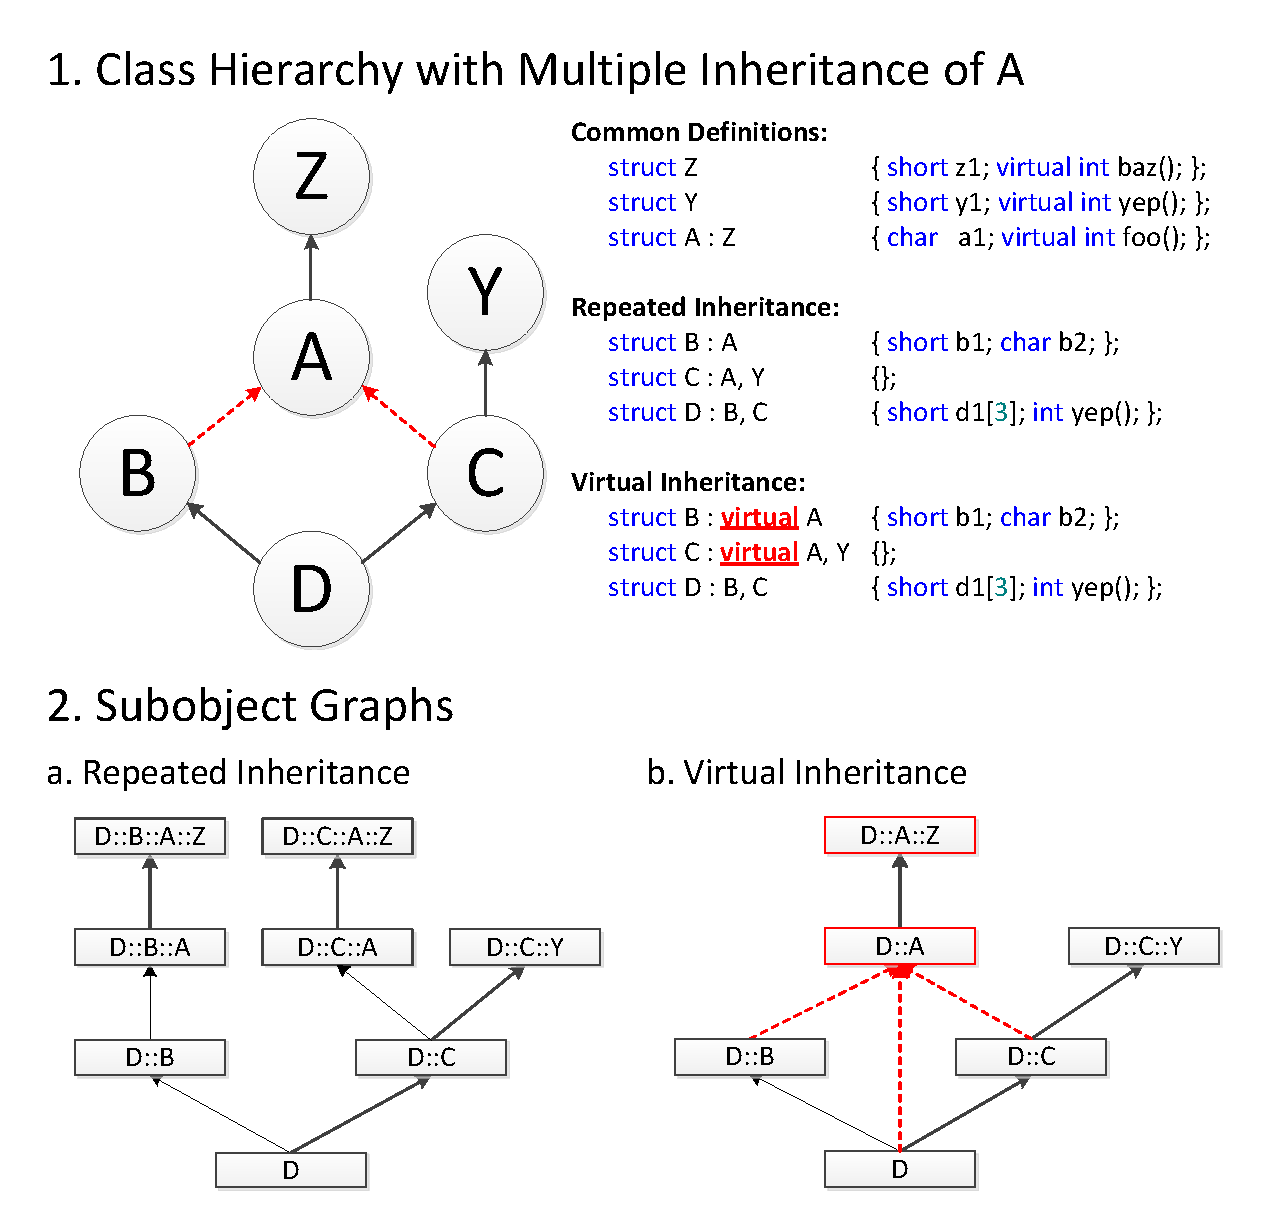
\includegraphics[width=0.47\textwidth]{Inheritance.pdf}
  \caption{Multiple Inheritance in \Cpp{}}
  \label{fig:inheritance}
\end{figure}

\noindent
Consider the simple class hierarchy in Figure~\ref{fig:inheritance}(1). Class 
\code{D} indirectly inherits from class \code{A} through its \code{B} and 
\code{C} base classes. In this case, the user may opt to keep distinct 
subobjects of class \code{A} (repeated inheritance) or a shared one (virtual 
inheritance) by specifying how \code{B} and \code{C} inherit from 
\code{A}. The kind of inheritance is thus not a property of a given class, but a 
property of an inheritance relation between classes and it is possible to mix the two. 

A class hierarchy gives rise to a \emph{subobject graph}, where a given class 
node may be replicated when inherited repeatedly or left shared when inherited 
virtually. The edges in such a graph represent \emph{subobject containment} and 
indicate whether such containment is shared or exclusive. 
Every class $C$ in the class hierarchy will have its own subobject 
graph representing the subobjects of an object of dynamic type $C$.
Figure~\ref{fig:inheritance}(2) shows subobject graph for class \code{D} 
obtained for the class hierarchy in Figure~\ref{fig:inheritance}(1) under repeated (a) and virtual (b) 
inheritance of class \code{A} by classes \code{B} and \code{C}. The shared 
containment is indicated with the dashed arrows, while exclusive -- with the solid 
ones.

\Cpp{}'s notion of multiple inheritance is fundamentally about 
subobjects, not just types.  Virtual inheritance is about
sharing the base-class subobjects, whereas non-virtual inheritance
reflects distinction in base-class subobjects from distinct class inheritance paths~\cite{CPPARM90}.

An object descriptor of static type $A$ referencing an object of the dynamic 
type $C$ can be understood as any $C$\code{::*::}$A$-node in the subobject graph of $C$. 
Casts can be understood as a change from one subobject to another.
We use the terms \emph{source subobject} and \emph{target 
subobject} to refer to the argument and result of the cast, respectively. Their 
static types will be referred to as \emph{source type} and \emph{target type} 
respectively. \Cpp{} distinguishes three kinds of casts: upcasts, downcasts, and 
crosscasts.

An \emph{upcast} is a cast from a derived class to one of its bases. When the 
base class is unambiguous, such casts are implicit and require no additional 
annotations. When the base class is ambiguous, cast failure is manifested 
statically in the form of a compile-time error. For example, this is the case with 
casting \code{D} to \code{A} under repeated multiple inheritance of \code{A}, 
in which case the user needs to explicitly cast the object to \code{B} or 
\code{C} first in order to indicate the desired subobject and resolve the ambiguity. 
In some cases, however, introduction of such an explicit cast is not possible: 
e.g. in implicit conversions generated by the compiler to implement covariant 
return types, crosscasts or conversions in generic code. This does not mean 
that in such cases we violate the Liskov substitution principle: the 
classes are still in a subtyping relation, but an implicit conversion is not 
available.

A \emph{downcast} is a cast from a base class to one of its derived classes. The 
cast has to determine at run-time whether the source subobject is contained by a 
subobject of the target type in the dynamic type's subobject graph. Failure 
of such a cast is manifested dynamically at run-time.

A \emph{crosscast} is a cast between classes that are not necessarily related by 
inheritance except by sharing a common derived class (subclass).
Accordingly to the \Cpp{} semantics such cast is defined to be a 
composition of upcast to target type and downcast to the dynamic type. 
While the downcast to the dynamic type is always guaranteed to succeed 
regardless of the source subobject, the upcast to the target type may be 
ambiguous, in which case the cast will fail at runtime. A cast from \code{Y} to 
\code{B} inside an object of dynamic type \code{D} in 
Figure~\ref{fig:inheritance}(2a,2b) is an example of a successful crosscast. A 
similar cast from \code{Y} to \code{A} inside \code{D} under the repeated  
inheritance in Figure~\ref{fig:inheritance}(2a) will fail because of the ambiguous 
upcast from \code{D} to \code{A}.

An interesting artifact of these distinctions can be seen in an example of 
casting a subobject of type \code{Z} to a subobject of type \code{A} in 
Figure~\ref{fig:inheritance}(2a). The subobject \code{D::B::A::Z} will be 
successfully cast to \code{D::B::A}, while the \code{D::C::A::Z} will be 
successfully cast to \code{D::C::A}. These casts do not involve downcasting to 
\code{D} followed by an upcast to \code{A}, which would be ambiguous, but 
instead take the dynamic type of a larger subobject (\code{D::B} or \code{D::C}) 
that the source subobject is contained in into account in order to resolve the 
ambiguity. A similar cast from \code{Y} to \code{A} will fail; should 
\code{Y} have also been non-virtually derived from \code{Z}, the cast from 
\code{D::C::Y::Z} to \code{A} would have failed. This shows that the distinction 
between crosscast and downcast is not based solely on the presence of a 
subtyping relation between the source and target types, but also on the actual 
position of the source subobject in the dynamic type's subobject graph.

The \Cpp{} inheritance model, presented here informally, further complicates the definition and
implementation of a type switch compared to simpler models. We have to define the
type switch so that only unambiguous casting between a source and a target within an object is possible.
That is, the implementation of the cast between source and target subobjects must take into account the
location of the source subobject in the subobject graph, rather than
just the dynamic and target types, which would suffice for a simple subtype testing.
Of course, every use of dynamic casting and every implicit cast are type safe~\cite{WNST06}.

%\section{Problem Description} %%%%%%%%%%%%%%%%%%%%%%%%%%%%%%%%%%%%%%%%%%%%%%%%%%
%\label{sec:probl}

\subsection{Existing Approaches to Type Case Analysis}
\label{sec:prev}

The closed nature of algebraic data types allows for their efficient 
implementation. The traditional compilation scheme assigns unique (and often 
small and sequential) tags to every variant of the algebraic data type and type 
switching is then simply implemented with a multi-way branch~\cite{Spuler94} 
(usually a jump table) over all the tags~\cite{Augustsson85}. Dealing with 
extensible hierarchical data types makes this %extremely efficient 
approach infeasible:

\begin{itemize}
\setlength{\itemsep}{0pt}
\setlength{\parskip}{0pt}
\item \emph{Extensibility} implies that the compiler may not know the exact set 
      of all the derived classes until link-time (due to \emph{separate compilation}) 
      or even run-time (due to \emph{dynamic linking}).
\item \emph{Substitutability} implies that we should be able to 
      match tags of derived classes against case labels representing tags of 
      base classes.
\item The presence of \emph{multiple inheritance} might require pointer adjustments 
      that are not known at compile time (e.g. due to virtual base classes, 
      ambiguous base classes or crosscasting).
\end{itemize}

%\noindent
%In some cases the substitutability requirement can be satisfied by obtaining 
%the base class' tag from a derived one first and then performing the jump. 
%This will work as long as we have only base classes in the case clauses.
%Derived classes that have to be treated separately from the rest of their 
%siblings will essentially be indistinguishable from them.
%
%When tags are not chosen arbitrarily but to reflect the subtyping relation of the 
%underlying hierarchy (e.g. certain bit set for certain base class), the assumed 
%structure of tags is likely to make the set of tags sparse. On one hand this 
%decreases the number of representable hierarchies and thus hinders openness, 
%while on the other it forces the compiler to use a decision tree instead of a jump 
%table to implement the switch. The former was consistently slower than the 
%latter one in our experience, even though the opposite was noted on some 
%architectures for small number of case clauses~\cite[\textsection 4]{garrigue-98}.

\noindent
There are two main approaches to implementing case analysis on extensible 
hierarchical data types discussed in the literature.

The first approach is based on either explicit or implicit sealing of the class 
hierarchy on which type switching can be performed. \Cpp{}11, for example, allows 
the user to prohibit further derivation by specifying a class to be ``final''~\cite{C++11}, 
similar to Scala and Java. The compiler then may use the above tag 
allocation over all variants to implement type analysis~\cite[\textsection 
4.3.2]{EmirThesis}. 
In some cases, the sealing may happen implicitly. For example, languages %that allow names 
with both internal and external linkage may employ the fact that classes 
with internal linkage will not be externally accessible and are thus effectively 
sealed. While clearly efficient, the approach is not open as it avoids the 
question rather than answers it. 

The broader problem with this approach is that techniques that rely on unique or
sequential compile or link-time constants violate independent extensibility 
since without a centralized authority there is no guarantee same constant will 
not be chosen in a type-unsafe manner by independent extensions. Updating such 
constants at load time may be too costly even when possible. %More often than 
%not, however such updates may require code regeneration since decision trees, 
%lookup tables etc. may have been generated by compiler for given values.

An important practical solution that follows this approach is the visitor design 
pattern~\cite{DesignPatterns1993}. The set of \code{visit} methods in a visitor's 
interface essentially seals the class hierarchy. Extensions have been proposed 
in the literature~\cite{Zenger:2001}, but they have problems of their own, 
as discussed in \textsection\ref{sec:rw}.

The second approach employs type inclusion tests combined with decision 
trees~\cite{Cardelli84} to avoid unnecessary checks. Its efficiency is then 
entirely focused on the efficiency of type inclusion 
tests~\cite{Schubert83,Wirth88,Cohen91,Caseau93,Vortex96,Krall97nearoptimal,Vitek97,PQEncoding,FastDynCast,Ducournau08}. 

%"A couple of years later, Nikolaus With published an approach based on type 
%inclusion. However, that approach does not work well in the presence of multiple 
%inheritance and separates the single logical operation of gaining type-safe 
%access to an object into two, implying the possibility of a programmer error." 

\Cpp{} has handled general dynamic casting since 1987, when multiple inheritance 
was added to the language~\cite{Str87}. Wirth later presented a technique that 
can be used to implement subtype tests by traversing a linked list of 
types~\cite{Wirth88}. His encoding required little space, but ran in time 
proportional to the distance between the two types in the class hierarchy. 
A trivial constant-time type inclusion test can be implemented with a 
\emph{binary matrix}, encoding the subtyping relation on the class 
hierarchy~\cite{Vortex96}. While efficient in time, it has quadratic space 
requirements, which makes it expensive for use on large class hierarchies. Cohen 
proposed the first space-efficient constant-time algorithm, but it can
only deal with single inheritance~\cite{Cohen91}. \emph{Hierarchical encoding} 
is another constant-time test that maps subtype queries into subset queries on 
bit-vectors~\cite{Caseau93,Krall97nearoptimal}. The approach can handle multiple
inheritance, but the space and time required for a subtype test in this encoding 
increases with the size of the class hierarchy; also, Caseau's approach~\cite{Caseau93} is 
limited to class hierarchies that are lattices. Schubert's \emph{relative 
numbering}~\cite{Schubert83} encodes each type with an interval $[l,r]$, 
effectively making type inclusion tests isomorphic to a simple range checking. 
The encoding is optimal in space and time, but it is limited to single 
inheritance. \emph{PQ-Encoding} of Zibin and Gil employs PQ-trees to improve 
further space and time efficiency of the constant-time inclusion 
testing~\cite{PQEncoding}. While capable of handling type inclusion queries on 
hierarchies with multiple inheritance, the approach makes the closed world assumption and can be costly 
for use with dynamic linking because it is not incremental.
The approach of Gibbs and Stroustrup~\cite{FastDynCast} employs divisibility of 
numbers to obtain a constant-time type inclusion test. The approach can handle 
multiple inheritance and was the first constant-time technique to addresses the 
problem of casts between subobjects. Unfortunately, the approach limits the size 
of the class hierarchies that can be encoded with this technique. 
Ducournau proposed a constant-time inclusion test based on the fact that, in an 
open solution, a class has a known number of base classes, and thus perfect hashes 
can be used to map them to this-pointer offsets typically used to implement 
subobject casts \cite{Ducournau08}. Unfortunately, the approach addresses only 
virtual multiple inheritance and (similarly to other approaches) relies on 
load-time computations. An excellent introduction to and detailed 
analysis of existing constant-time type inclusion tests can be found in 
\cite{Vitek97,PQEncoding}.

With the exception of work by Gibbs and Stroustrup~\cite{FastDynCast}, all the 
approaches to efficient type-inclusion testing we found in the literature were 
based on the assumption that \emph{the outcome of a subtyping test as well as 
the subsequent cast depend only on the target type and the dynamic type of 
the object}. Although that assumption is sound for subtyping tests and subtype 
casts for shared inheritance (including single), it does not reflect the 
relationship between subobjects in the general case of multiple inheritance 
as found in \Cpp{}.

\subsection{The Source of Inefficiency}

While constant-time type inclusion tests are invaluable in optimizing subtype 
tests in programming languages, their use in implementing a type switch is 
inferior to some workaround techniques. This may prevent wide adoption of a 
language implementation of such a feature due to its inferior performance. 
We implemented 3 constant-time type inclusion tests: binary 
matrix~\cite{Vitek97}, Cohen's algorithm~\cite{Cohen91}, and fast dynamic 
cast~\cite{FastDynCast} and combined them with a decision tree to implement a 
type switch on a class hierarchy ideally suited for such scenarios: a perfect binary tree with 
classes number $2i$ and $2i+1$ derived from a class number $i$. Our workaround 
techniques included the visitor design pattern and a switch on the sealed sequential 
set of tags.

\begin{figure}[htbp]
  \centering
    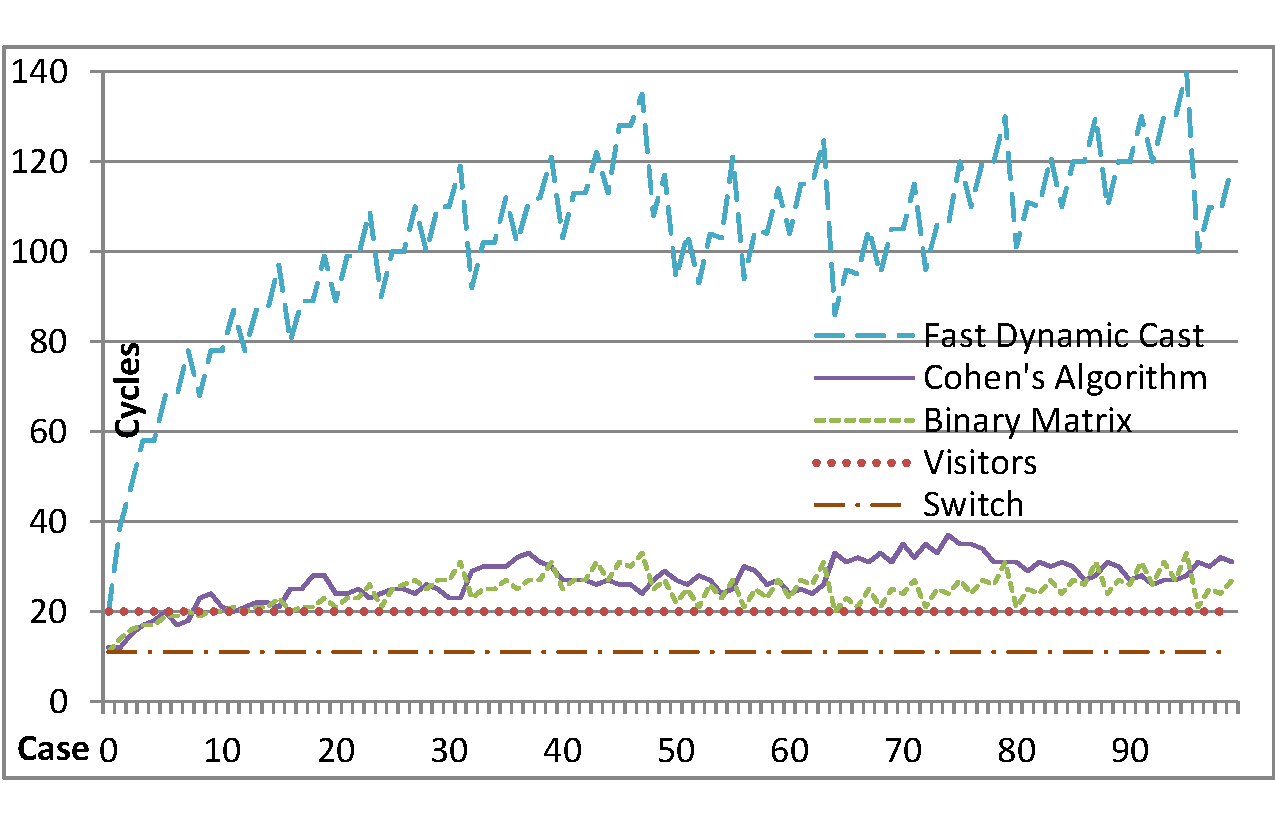
\includegraphics[width=0.47\textwidth]{DCast-vs-Visitors.pdf}
  \caption{Type switch based on constant-time subtype tests}
  \label{fig:DCastVis2}
\end{figure}

The chart in Figure~\ref{fig:DCastVis2} shows the number of cycles (Y-axis) each 
technique took to recognize an object of the dynamic type $i$ (X-axis). 
Despite known limitations, binary matrix and Cohen's algorithm are some of the 
fastest known type inclusion tests for single inheritance~\cite{Vitek97}. It 
is nonetheless easy to see that the logarithmic cost associated with the 
decision tree very quickly surpasses the constant overhead of double dispatch 
(20 cycles) present in the visitor design pattern or the jump-table 
implementation of the switch on all tags (11 cycles). We expect the cost of 
techniques capable of handling multiple inheritance to be even higher, especially 
those addressing casting between subobjects (e.g. fast dynamic cast). The edgy 
shape of timing results reflects the shape of the class hierarchy used for this 
experiment.
%We show in \textsection{sec:viscmp} that 
%our open solution is capable of delivering an amortized constant-time type 
%switching wi
\subsection{An Attractive Non-Solution}
\label{sec:cotc}

The memoization device outlined in \textsection\ref{sec:memdev} can, in principle, also be 
applied to tagged classes. The dynamic cast will be replaced by a small 
compile-time template meta-program that checks whether the class associated with 
the given tag is derived from the target type of the case clause. If so, a static 
cast can be used to obtain the offset.

Despite its straightforwardness, we felt that it should be possible to do better 
than the general solution, given that each class is already identified with a 
dedicated constant known at compile time.

While Wirth' linked list encoding was considered slow for subtype testing, it can 
be adopted for quite efficient type switching on a class hierarchy with no 
repeated inheritance. The idea is to combine fast switching on closed 
algebraic datatypes with a loop that tries the tags of base classes when 
switching on derived tags fails.

As we mentioned in \textsection\ref{sec:poets}, 
the nominal subtyping of \Cpp{} effectively gives every class multiple types. The 
idea is thus to associate with the type not only its most-derived tag, but also 
the tags of all its base classes. In a compiler implementation such a 
list can be stored inside the virtual table of a class, while in our library 
solution it is shared between all the instances with the same most-derived tag 
in a less efficient global map, associating the tag to its tag list.

For simplicity of presentation we assume a pointer to an array of tags be available 
directly through the subject's \code{taglist} data member. The array is of 
variable size: its first element is always the tag of the subject's dynamic 
type, while its end is marked with a dedicated \code{end_of_list} marker, 
distinct from all the tags. The tags in between are topologically sorted 
according to the subtyping relation with incomparable siblings listed in 
\emph{local precedence order} -- the order of the direct base classes used in 
the class definition. We call such a list a \emph{Tag Precedence List} (TPL) as it resembles the \emph{Class Precedence List} (CPL) of 
object-oriented descendants of Lisp (e.g. Dylan, Flavors, LOOPS, and CLOS) used 
there for \emph{linearization} of class hierarchies. 
The classes in CPL are ordered from most specific to least specific 
with siblings listed in the \emph{local precedence order} -- the order of the 
direct base classes used in the class definition. TPL is just an implementation 
detail and the only reason we distinguish TPL from CPL is that in C++ classes 
are often separated into interface and implementation classes and it might so 
happen that the same tag is associated by the user with an interface and several 
implementation classes. 

We also assume the tag-constant associated with a class \code{Di} is accessible 
through a static member \code{Di::class_tag}. These simplifications are not 
essential and the library does not rely on any of them.
%Instead, the user can retroactively narrate to the library the specific tag 
%encoding used through a trait-like class.

A type switch, below, built on top of a hierarchy of tagged classes, proceeds as 
a regular switch on the subject's tag. If the jump succeeds, we found an exact 
match; otherwise, we get into a default clause that obtains the next tag in the 
tag precedence list and jumps back to the beginning of the switch statement for a 
rematch:

\begin{lstlisting}[keepspaces]
          size_t  attempt = 0;
    size_t tag = subject->taglist[attempt];
ReMatch:
    switch (tag) {
    default:
        tag = subject->taglist[++attempt];
        goto ReMatch;
    case end_of_list: 
        break;
    case D1::class_tag: 
        D1& match = static_cast<D1&>(*subject); s1;
        break;
    ...
    case Dn::class_tag: 
        Dn& match = static_cast<Dn&>(*subject); sn;
        break;
    }
\end{lstlisting}

\noindent
The above structure, which we call a \emph{tag switch}, implements a variation of 
best-fit semantics based on local precedence order. It lets us dispatch to the case 
clause of the most-specialized class with an overhead of initializing two 
local variables, compared to an efficient switch used on algebraic data types. 
Dispatching to a case clause of a base class will take time roughly proportional 
to the distance between the matched base class and the derived class in the 
inheritance graph, thus the technique is not constant. When none of the base 
class tags was matched, we will necessarily reach the end\_of\_list marker %in the list 
and exit the loop. %As mentioned before, 
The default clause, %of the type switch 
again, can be implemented with a case clause on the subject type's tag: \code{case S::class_tag:}

The efficiency of the above code crucially depends on the set of tags 
being small and sequential to justify the use of a jump table instead of a
decision tree to implement the switch. This is usually not a problem in closed 
hierarchies based on tag encoding since the designer of the hierarchy handpicks 
the tags herself. The use of a static cast %to obtain proper reference once the most specialized derived class has been established, 
however, essentially limits the use of 
this mechanism to non-repeated inheritance only. This only refers to the way target 
classes inherit from the subject type -- they can freely inherit from other classes. 
%as long as they inherit the subject type through non-repeated inheritance only. 
Due to these restrictions, the technique is not open because it may  
violate independent extensibility. We discuss in \textsection\ref{sec:cmp} that 
making the technique more open will also eradicate its performance advantages.

Our library automatically builds the function \code{get_taglist} based on the 
\code{BC} or \code{BCS} specifiers that the user specifies in bindings 
(\textsection\ref{sec:bnd}).

\section{Type Switching}
\label{sec:copc}

%While \Cpp{} does not have direct support for algebraic data types, they can be 
%encoded with classes in a number of ways. One common such encoding is to 
%introduce an abstract base class representing an algebraic data type with 
%several derived classes representing variants. The variants can be 
%discriminated with either run-time type information (\emph{polymorphic 
%encoding}) or a unique tag inside a dedicated member of the common base class 
%(\emph{tagged encoding}).

\emph{Mach7} explicitly supports at least two encodings of algebraic
datatypes: runtime type information discriminant, and numerical tag
data member shared by all classes in a given hierarchy.  The library
handles them differently to let 
the user choose between openness and efficiency. The type switch for tagged 
encoding (\textsection\ref{sec:cotc}) is simpler and more efficient for many typical use cases, however, 
making it open eradicates its performance advantages (\textsection\ref{sec:cmp}). 
%The difference in 
%performance is the price we pay for keeping the solution open. We describe pros 
%and cons of each approach in \textsection\ref{sec:cmp}.

%The core of the proposal relies on two key aspects of \Cpp{} implementations:
%\begin{enumerate}
%\item a constant-time access to the virtual table pointer embedded in an object of
%  dynamic class type;
%\item injectivity of the relation between an object's inheritance path
%  and the virtual table pointer extracted from that object.
%\end{enumerate}

%\subsection{An Attractive Non-Solution}
\label{sec:cotc}

%The memoization device outlined in \textsection\ref{sec:memdev} can, in principle, also be 
%applied to tagged classes. The dynamic cast will be replaced by a small 
%compile-time template meta-program that checks whether the class associated with 
%the given tag is derived from the target type of the case clause. If so, a static 
%cast can be used to obtain the offset.

%Despite its straightforwardness, we felt that it should be possible to do better 
%than the general solution, given that each class is already identified with a 
%dedicated constant known at compile time.

While Wirth' linked list encoding was considered slow for subtype testing, it can 
be adopted for quite efficient type switching on a class hierarchy with no 
repeated inheritance. The idea is to combine fast switching on closed 
algebraic datatypes with a loop that tries the tags of base classes when 
switching on derived tags fails.

%The nominal subtyping of \Cpp{} effectively gives every class multiple types. The 
%idea is thus to associate with the type not only its most-derived tag, but also 
%the list of tags of all its base classes. In a compiler implementation such a 
%list can be stored inside the virtual table of a class, while in our library 
%solution it is shared between all the instances with the same most-derived tag 
%in a less efficient global map, associating the tag to its tag list.

For simplicity of presentation we assume a pointer to an array of tags be available 
directly through the subject's \code{taglist} data member. The array is of 
variable size: its first element is always the tag of the subject's dynamic 
type, while its end is marked with a dedicated \code{end_of_list} marker, 
distinct from all the tags. The tags in between are topologically sorted 
according to the subtyping relation with incomparable siblings listed in 
\emph{local precedence order} -- the order of the direct base classes used in 
the class definition. The list resembles the \emph{class precedence list} of 
object-oriented descendants of Lisp (e.g. Dylan, Flavors, LOOPS, and CLOS) used 
there for \emph{linearization} of class hierarchies. 
We also assume the tag-constant associated with a class \code{Di} is accessible 
through a static member \code{Di::class_tag}. These simplifications are not 
essential and the library does not rely on any of them.
%Instead, the user can retroactively narrate to the library the specific tag 
%encoding used through a trait-like class.

A type switch, below, %, built on top of a hierarchy of tagged classes, 
proceeds as 
a regular switch on the subject's tag. If the jump succeeds, we found an exact 
match; otherwise, we get into a default clause that obtains the next tag in the
list and jumps back %to the beginning of the switch statement 
for a rematch:

\begin{lstlisting}[keepspaces]
    size_t attempt = 0; 
    size_t tag = subject->taglist[attempt];
ReMatch:
    switch (tag) {
    default:
        tag = subject->taglist[++attempt];
        goto ReMatch;
    case end_of_list: 
        break;
    case D1::class_tag: 
        D1& match = static_cast<D1&>(*subject); s1;
        break;
        ...
    case Dn::class_tag: 
        Dn& match = static_cast<Dn&>(*subject); sn;
        break;
    }
\end{lstlisting}

\noindent
The above structure, which we call a \emph{tag switch}, implements a variation of 
best-fit semantics based on local precedence order. It lets us dispatch to the case 
clause of the most-specialized class with an overhead of initializing two 
local variables, compared to an efficient switch used on algebraic data types. 
Dispatching to a case clause of a base class will take time roughly proportional 
to the distance between the matched base class and the derived class in the 
inheritance graph, thus the technique is not constant. When none of the base 
class tags was matched, we will necessarily reach the end\_of\_list marker %in the list 
and exit the loop. %As mentioned before, 
The default clause, %of the type switch 
again, can be implemented with a case clause on the subject type's tag: \code{case S::class_tag:}

The efficiency of the above code crucially depends on the set of tags 
being small and sequential to justify the use of a jump table instead of a
decision tree to implement the switch. This is usually not a problem in closed 
hierarchies based on tag encoding since the designer of the hierarchy handpicks 
the tags herself. The use of a static cast %to obtain proper reference once the most specialized derived class has been established, 
however, essentially limits the use of 
this mechanism to non-repeated inheritance only. This only refers to the way target 
classes inherit from the subject type -- they can freely inherit from other classes. 
%as long as they inherit the subject type through non-repeated inheritance only. 
Due to these restrictions, the technique is not open because it may  
violate independent extensibility. We discuss in \textsection\ref{sec:cmp} that 
making the technique more open will also eradicate its performance advantages.


\subsection{An Open but Inefficient Solution}
\label{sec:poets}

Instead of starting with an efficient solution and trying to make it open, we 
start with an open solution and try to make it efficient. The following 
cascading-if statement implements the first-fit semantics for our type switch in 
a truly open fashion:

\begin{lstlisting}
if (T1* match=dynamic_cast<T1*>(subject)) {s1;} else
if (T2* match=dynamic_cast<T2*>(subject)) {s2;} else
...
if (Tn* match=dynamic_cast<Tn*>(subject)) {sn;}
\end{lstlisting}

\noindent
Despite the obvious simplicity, its main drawback is performance: a typical implementation of 
\code{dynamic_cast} takes time proportional to the distance between base and 
derived classes in the inheritance tree. What is worse is that due to the
sequential order of tests, the time to uncover the type in the $i^{th}$ case 
clause will be proportional to $i$, while failure to match will take the longest. 
This linear increase can be seen in the Figure~\ref{fig:DCastVis1}, where 
the above cascading-if was applied to a flat hierarchy encoding an algebraic 
data type with 100 variants. The same type-switching functionality implemented 
with the visitor design pattern took only 28 cycles regardless of the 
case.\footnote{Each case $i$ was timed multiple times, thus turning the experiment 
into a repetitive benchmark described in \textsection\ref{sec:eval}. In a more
realistic setting, represented by random and sequential benchmarks, the cost of 
double dispatch was varying between 52 and 55 cycles.}
This is more than 3 times faster than the 93 cycles it took to uncover even the 
first case with \code{dynamic_cast}, while it took 22760 cycles to uncover the 
last.
In a test involving a flat hierarchy of 100 variants, it took 93 cycles to 
discover the first type and 22760 to discover the last (with their linear combination 
for the types in between). A visitor design pattern could 
uncover any type in about 55 cycles, regardless of its position among the case 
clauses, while a switch based on sequential tags could achieve the same in less 
than 20 cycles. The idea is thus to combine the openness of the above structure 
with the efficiency of a jump table on small sequential values.

Relying on \code{dynamic_cast} also makes an implicit semantic choice where we 
are no longer looking for the first/best-fitting type that is in subtyping 
relation, but for the first/best-fitting type to which a cast is possible from 
the source subobject (\textsection\ref{sec:specifics}).

\begin{figure}[htbp]
  \centering
    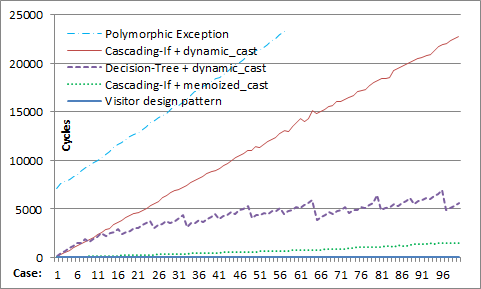
\includegraphics[width=0.47\textwidth]{DCast-vs-Visitors1.png}
  \caption{Type switching based on na\"ive techniques}
  \label{fig:DCastVis1}
\end{figure}

%Seeing several solutions whose time increases with the position of the case 
%clause in the type switch, one may wonder how many such clauses a typical 
%program might have. A program dealing with abstract syntax trees in 
%Pivot~\cite{Pivot09} that we implemented using our pattern-matching library had 
%8 match statements with 5, 7, 8, 10, 15, 17, 30 and 63 case clauses, 
%respectively. With Pivot having the smallest number of node kinds among the 
%compiler frameworks we had a chance to work with, we expect a similar or larger 
%number of case clauses in other compiler applications.

When the class hierarchy is not flat and has several levels, the above cascading-if can be replaced 
with a decision tree that tests base classes first and thus eliminates many of 
the derived classes from consideration. This approach is used by Emir to deal with 
type patterns in Scala~\cite[\textsection 4.2]{EmirThesis}. The intent is to 
replace a sequence of independent dynamic casts between classes that are far 
from each other in the hierarchy with nested dynamic casts between classes that 
are close to each other. Another advantage is the possibility to fail early: 
if the type of the subject does not match any of the clauses, we will not have to try all the cases. 
A flat hierarchy, which will likely be formed by the leaves in even a multi-level 
hierarchy, will not be able to benefit from this optimization and 
will effectively degrade to the above cascading-if. Nevertheless, when 
applicable, the optimization can be very useful and its benefits can be seen in
Figure~\ref{fig:DCastVis1} under ``Decision-Tree + dynamic\_cast''. The class 
hierarchy for this timing experiment formed a perfect binary tree with 
classes number 2*N and 2*N+1 derived from a class with number N. The structure 
of the hierarchy also explains the repetitive pattern of timings.

The above solution either in a form of cascading-if or as a decision tree can be 
significantly improved by lowering the cost of a single \code{dynamic_cast}. 
We devised an asymptotically constant version of this operator that we call
\code{memoized_cast} in \textsection\ref{sec:memcast}. As can be seen 
from the graph titled ``Cascading-If + memoized\_cast'', it speeds up the 
above cascading-if solution by a factor of 18 on average, as well as outperforms 
the decision-tree based solution with dynamic\_cast for a number of case clauses 
way beyond those that can happen in a reasonable program. 
We leave the discussion of the technique until 
\textsection\ref{sec:memcast}, while we keep it in the chart to give perspective on 
an even faster solution to dynamic casting. The slowest implementation in the 
chart based on exception handling facilities of C++ is discussed in 
\textsection\ref{sec:xpm}.

The approach of Gibbs and Stroustrup~\cite{FastDynCast} employs divisibility of numbers to obtain a 
tag allocation scheme capable of performing type testing in constant time. 
Extended with a mechanism for storing offsets required for this-pointer 
adjustments, the technique can be used for extremely fast dynamic casting on 
quite large class hierarchies. The idea is to allocate tags 
for each class in such a way that tag of a class D is divisible by a tag of a 
class B if and only if class D is derived from class B. For comparison purposes 
we hand crafted this technique on the above flat and binary-tree hierarchies and 
then redid the timing experiments from Figure~\ref{fig:DCastVis1} using the fast 
dynamic cast. The results are presented in Figure~\ref{fig:DCastVis2}. For 
reference purposes we retained ``Visitor Design Pattern'' and ``Cascading-If + 
memoized\_cast'' timings from Figure~\ref{fig:DCastVis1} unchanged. Note that 
the Y-axis has been scaled-up 140 times, which is why the slope of 
``Cascading-If + memoized\_cast'' timings is so much steeper.

\begin{figure}[htbp]
  \centering
    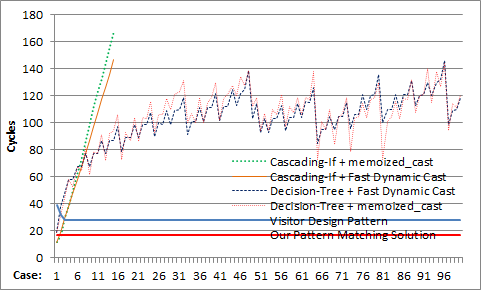
\includegraphics[width=0.47\textwidth]{DCast-vs-Visitors2.png}
  \caption{Type switching based on the fast dynamic cast of Gibbs and Stroustrup~\cite{FastDynCast}}
  \label{fig:DCastVis2}
\end{figure}

As can be seen from the figure the use of our memoized\_cast implementation can 
get close in terms of performance to the fast dynamic cast, especially 
when combined with decision trees. An important difference that cannot be seen 
from the chart, however, is that the performance of memoized\_cast is 
asymptotic, while the performance of fast dynamic cast is guaranteed. This 
happens because the implementation of memoized\_cast will incur an overhead of 
a regular dynamic\_cast call on every first call with a given most derived type. 
Once that class is memoized, the performance will remain as shown. Averaged over 
all calls with a given type we can only claim we are asymptotically as good as 
fast dynamic cast.

Unfortunately fast dynamic casting is not truly open to fully satisfy our 
checklist. The structure of tags required by the scheme limits the number of 
classes it can handle. A 32-bit integer is estimated to be able to represent 7 
levels of a class hierarchy that forms a binary tree (255 classes), 6 levels of 
a similar ternary tree hierarchy (1093 classes) or just one level of a hierarchy 
with 9 base classes -- multiple inheritance is the worst case scenario of the 
scheme that quickly drains its allocation possibilities. Besides, similarly to 
other tag allocation schemes, presence of class extensions in \emph{Dynamically Linked Libraries} (DLLs) will likely 
require an integration effort to make sure different DLLs are not reusing prime 
numbers in a way that might result in an incorrect dynamic cast.

A number of other constant-time techniques for class-membership testing is 
surveyed by Gil and Zibin~\cite[\textsection 4]{PQEncoding}. They are intended 
for type testing, and thus will have to be combined with decision trees 
for type switching, resulting in similar to fast dynamic cast performance. 
They too assume access to the entire class hierarchy at compile time and thus 
are not open.

In view of the predictably-constant dispatching overhead of the visitor design pattern, 
it is clear that any open solution that will have a non-constant dispatching 
overhead will have a poor chance of being adopted. Multi-way switch on 
sequentially allocated tags~\cite{Spuler94} was one of the few techniques that 
could achieve constant overhead, and thus compete with and even outperform visitors. 
Unfortunately the scheme has problems of its own that make it unsuitable for 
truly open type-switching and here is why.

%To better understand the problem let us look at some existing solutions to type 
%switching that we found to be used in practice. 

%From our experience on this project we have noticed that we can only compete 
%with visitors when switch statements are implemented with a jump table. As soon 
%as compiler was putting even a single branch into the decision tree of cases, 
%the performance was degraded significantly. From this perspective we do not 
%regard solutions based on decision trees as efficient, since they do not let us 
%compete compete with the visitors solution.

The simple scheme of assigning a unique tag per variant (instantiatable class 
here) will not pass our first question because the tags of base and derived 
classes will have to be different if the base class can be instantiated on its 
own. In other words we will not be able to land on a case label of a base class, while 
having a derived tag only. The already mentioned partitioning of tags of derived 
classes based on the classes in case clauses also will not help as it assumes 
knowledge of all the classes and thus fails extensibility through DLLs.

In practical implementations hand crafted for a specific class hierarchy, tags 
often are not chosen arbitrarily, but to reflect the subtyping relation of the 
underlying hierarchy. Switching on base classes in such a setting will typically 
involve a call to some function $f$ that converts derived class' tag into a base 
class' tag. An example of such a scheme would be having a certain bit in the tag 
set for all the classes derived from a given base class. Unfortunately this 
solution creates more problems than it solves.

First of all the solution will not be able to recognize an exceptional case 
where most of the derived classes should be handled as a base class, while a few 
should be handled specifically. Applying the function $f$ puts several different 
types into an equivalence class with their base type, making them 
indistinguishable from each other.

Secondly, the assumed structure of tags is likely to make the set of tags 
sparse, effectively forcing the compiler to use a decision tree instead of a jump 
table to implement the switch. Even though conditional jump is reported to be 
faster than indirect jump on many computer architectures~\cite[\textsection 
4]{garrigue-98}, this did not seem to be the case in our experiments. Splitting 
of a jump table into two with a condition, that was sometimes happening because 
of our case label allocation scheme, was resulting in a noticeable degradation of 
performance in comparison to a single jump table.

Besides, as was seen in the scheme of Gibbs and Stroustrup, the assumed 
structure of tags can also significantly decrease the number of classes a given 
allocation scheme can handle. It is also interesting to note that even though 
their scheme can be easily adopted for type switching with decision trees, it is 
not easily adoptable for type switching with jump tables: in order to obtain 
tags of base classes we will have to decompose the derived tag into primes and 
then find all the dividers of the tag present in case clauses.

Several authors had noted the relationship between exception handling and type 
switching before~\cite{Glew99,ML2000}. Not surprisingly, the exception handling 
mechanism of \Cpp{} can be abused to implement the first-fit semantics of a type 
switch statement. The idea is to harness the fact that catch-handlers in \Cpp{} 
essentially use first-fit semantics to decide which one is going to handle a 
given exception. Unfortunately the approach is even slower than the use of 
\code{dynamic_cast} and we only list it here for comparison.

To summarize, truly open and efficient type switching is a non-trivial problem. 
The approaches we found in the literature were either open or efficient, 
but not both. Efficient implementation was typically achieved by sealing the 
class hierarchy and using a jump table on sequential tags. Open implementations 
were resorting to type testing and decision trees, which was not efficient. 
We are unaware of any efficient tag allocation scheme that can be used in a 
truly open scenario.

%%%%%%%%%%%%%%%%%%%%%%%%%%%%%%%%%%%%%%5555

%\noindent
%We chose to give it a first-fit semantics in our library as it was resembling 
%pattern matching facilities of other languages and was the most intuitive. The 
%following code can be generated to implement it:
%
%\begin{lstlisting}
%if (D1* derived = dynamic_cast<D1*>(base)) { s1; } else
%if (D2* derived = dynamic_cast<D2*>(base)) { s2; } else
%...
%if (Dn* derived = dynamic_cast<Dn*>(base)) { sn; }
%\end{lstlisting}

%\noindent
%Note that leaving \code{else} out will effectively turn it into an all-fit 
%statement with enabled statements executed in lexicographical order.
%
%The above code is easy to understand but is extremely inefficient as for an 
%object of dynamic type $D_i$ we will have to perform $i-1$ dynamic casts that 
%fail first. The diagram below compares the times spent by visitors and the above 
%type switch statement to uncover the $i^{th}$ case. We postpone the discussion 
%of \code{memoized_cast} until section \textsection\ref{}, here we would only 
%like to notice that even though faster than the actual dynamic cast it also bears 
%a linear coefficient, not present in visitors.

\section{Solution for Polymorphic Classes}
\label{sec:copc}

Our handling of type switches for polymorphic and tagged encodings differs 
with each having its pros and cons described in details in \textsection\ref{sec:cmp}.
In this section we will concentrate on the truly open type switch for 
polymorphic encoding. The type switch for tagged encoding (\textsection\ref{sec:cotc}) 
is simpler and more efficient, however, making it open will eradicate its 
performance advantages. The difference in performance is the price we pay for 
keeping the solution open.  The core of the proposal relies on two key
aspects of C++ implementations:
\begin{enumerate}
\item a constant-time access to the virtual table pointer embedded in an object of
  dynamic class type;
\item injectivity of the relation between an object's inheritance path
  and the virtual table pointer extracted from that object.
\end{enumerate}

\subsection{A Memoization Device}
\label{sec:memdev}

Let us look at a slightly more general problem than type switching. Consider a 
generalization of the switch statement that takes predicates on a subject as its 
clauses and executes the first statement $s_i$ whose predicate is enabled: 

\begin{lstlisting}[keepspaces]
switch (x)
{
    case P1(x): s1;
    ...
    case Pn(x): sn;
}
\end{lstlisting}

\noindent
Assuming that predicates are \emph{functional} (i.e. do not involve any side 
effects), the next time we execute the switch with the same value $x$, the same 
predicate will be enabled first. We thus would like to avoid evaluating 
preceding predicates and jump to the statement it guards. In a way, we 
would like the switch to memoize the case enabled for a given $x$. 

The idea is to generate a simple cascading-if statement interleaved with jump 
targets and instructions that associate the original value with enabled target. 
The code before the statement looks up whether the association for a given value 
has already been established, and, if so, jumps directly to the target; otherwise, 
the sequential execution of the cascading-if is started. To ensure 
that the actual code associated with the predicates remains unaware of this 
optimization, the code preceding it after the target must re-establish any 
invariant guaranteed by sequential execution (\textsection\ref{sec:vtblmem}).

Described code can be easily produced in a compiler setting, but generating it in 
a library is a challenge. Inspired by Duff's Device~\cite{Duff}, 
we devised a construct that we call \emph{Memoization Device} doing just 
that in standard \Cpp{}:

\begin{lstlisting}
typedef decltype(x) T; // T is the type of subject x
static std::unordered_map<T,size_t> jump_targets;

switch (size_t& jump_to = jump_targets[x]) {
default: // entered when we have not seen x yet
    if (P1(x)) { jump_to = 1; case 1: s1; } else 
    if (P2(x)) { jump_to = 2; case 2: s2; } else
 ...
    if (Pn(x)) { jump_to = @$n$@; case @$n$@: sn; } else
                jump_to = @$n+1$@;
case @$n+1$@: // none of the predicates is true on x
}
\end{lstlisting}

\noindent
The static \code{jump_targets} hash table will be allocated upon first entry 
to the function. The map is initially empty and according to its logic, 
request for a key $x$ not yet in the map will allocate a 
new entry with its associated data default initialized (to 0 for \code{size_t}). Since 
there is no case label 0 in the switch, the default case will be taken, which, in 
turn, will initiate sequential execution of the interleaved cascading-if 
statement. Assignments to \code{jump_to} effectively establish association 
between value $x$ and corresponding predicate, since \code{jump_to} is a 
reference to \code{jump_targets[x]}. The last assignment records absence of 
enabled predicates for $x$.

The sequential execution of the cascading-if statement will keep checking 
predicates $P_j(x)$ until the first predicate $P_i(x)$ that returns true. By 
assigning $i$ to \code{target} we will effectively associate $i$ with $x$ since 
\code{target} is just a reference to \code{jump_target_map[x]}. This association 
will make sure that the next time we are called with the value $x$ we will jump 
directly to the label $i$. When none of the predicates returns true, we will 
record it by associating $x$ with $N+1$, so that the next time we can jump 
directly to the end of the switch on $x$. 

The above construct effectively gives the entire statement first-fit semantics. 
In order to evaluate all the statements whose predicates are true, and thus 
give the construct all-fit semantics, we might want to be able to preserve the 
fall-through behavior of the switch. In this case we can still skip the initial 
predicates returning false and start from the first successful one. This can be 
easily achieved by removing all else statements and making if-statements 
independent as well as wrapping all assignments to \code{target} with a condition, 
to make sure only the first successful predicate executes it:

\begin{lstlisting}
if (Pi(x)) { if (jump_to == 0) jump_to = @$i$@; case @$i$@: si; }
\end{lstlisting}

\noindent
Note that the protocol that has to be maintained by this structure does not 
depend on the actual values of case labels. We only require them to be 
different and include a predefined default value. The default clause can be 
replaced with a case clause for the predefined value, but keeping the default  
clause generates faster code. A more important consideration is to 
keep the values close to each other. Not following this rule might result in a 
compiler choosing a decision tree over a jump table implementation of the 
switch, which in our experience significantly degrades the performance.

The first-fit semantics is not an inherent property of the memoization device. 
Assuming that the conditions are either mutually exclusive or imply one another, we 
can build a decision-tree-based memoization device that will effectively have 
\emph{most-specific} semantics -- an analog of best-fit semantics in predicate 
dispatching~\cite{ErnstKC98}.

Imagine that the predicates with the numbers $2i$ and $2i+1$ are mutually exclusive and 
each imply the value of the predicate with number $i$, i.e.
$\forall i\forall x\in\bigcap_j\mathsf{Domain}(P_j).P_{2i+1}(x)\rightarrow P_i(x)\wedge P_{2i}(x)\rightarrow P_i(x)\wedge\neg(P_{2i+1}(x)\wedge P_{2i}(x))$ holds. 
Examples of such predicates are class membership tests where the truth of 
testing membership in a derived class implies the truth of testing membership in 
its base class.

The following decision-tree-based memoization device will execute the statement 
$s_i$ associated with the \emph{most-specific} predicate $P_i$ (i.e. the 
predicate that implies all other predicates true on $x$) that evaluates to true 
or will skip the entire statement if none of the predicates is true on $x$.

\begin{lstlisting}
switch (size_t& jump_to = jump_targets[x]) {
default:
    if (P1(x)) {
        if (P2(x)) {
            if (P4(x)) { jump_to = 4; case 4: s4; } else
            if (P5(x)) { jump_to = 5; case 5: s5; } 
            jump_to = 2; case 2: s2;
        } else
        if (P3(x)) {
            if (P6(x)) { jump_to = 6; case 6: s6; } else
            if (P7(x)) { jump_to = 7; case 7: s7; } 
            jump_to = 3; case 3: s3;
        }
        jump_to = 1; case 1: s1;
    } else { jump_to = 0; case 0: ; }
}
\end{lstlisting}

\noindent
An example of predicates that satisfy this condition are class membership tests
where the truth of a predicate that tests membership in a derived class implies 
the truth of a predicate that tests membership in its base class. 
Our library solution prefers the simpler cascading-if approach only because the 
necessary code structure can be laid out with macros. A compiler solution 
will use the decision-tree approach whenever possible to lower the cost of the 
first match from linear in case's number to logarithmic as seen in Figure\ref{fig:DCastVis1}.

When the predicates do not satisfy the implication or mutual exclusion properties 
mentioned above, a compiler of a language based on predicate dispatching would 
typically issue an ambiguity error. Some languages might choose to resolve it 
according to lexical or some other ordering. In any case, the presence of 
ambiguities or their resolution has nothing to do with memoization device 
itself. The latter only helps optimize the execution once a particular choice of 
semantics has been made and code implementing it has been laid out.

The main advantage of the memoization device is that it can be built around 
almost any code, providing that we can re-establish the invariants guaranteed 
by sequential execution. Its main disadvantage is the size of the hash table 
that grows proportionally to the number of different values seen. Fortunately, 
the values can often be grouped into equivalence classes that do not change the 
outcome of the predicates. The map can then associate the equivalence class of a 
value with a target instead of associating the value with it. 

In application to type switching, the idea is to use the memoization device to 
learn the outcomes of type inclusion tests (with \code{dynamic_cast} used as a 
predicate). The objects can be grouped into equivalence classes based on their 
dynamic type: the outcome of each type inclusion test will be the same on 
all the objects of the same dynamic type. We can use the  
address of a class' \code{type_info} object obtained in constant time with the
\code{typeid()} operator as a unique identifier of each dynamic type. 
Presence of multiple \code{type_info} objects for the same class, as is often 
the case when dynamic linking is involved, is not a problem, as it would 
effectively split a single equivalence class into multiple ones. 

This could have been a solution if we were only interested in class membership. 
More often than not, however, we will be interested in obtaining a reference to 
the target type of the subject, and we saw in \textsection\ref{sec:specifics} 
that the cast between the source and target subobjects depends on 
the position of the source subobject in the dynamic type's subobject graph. 
We thus would like to have different equivalence classes for different 
subobjects, but there seems to be no easy way of identifying them given just an object descriptor.

\subsection{Virtual Table Pointers}
\label{sec:vtp}

%In this section we show that under certain conditions the compiler cannot share 
%the same virtual tables between different classes or their subobjects. This 
%allows us to use virtual table pointers to \emph{uniquely} identify the 
%subobjects within the most-derived class.

Before we discuss our solution we would like to talk about certain properties of 
the C++ run-time system that we rely on. In particular,
we show that under certain conditions the compiler cannot share 
the same virtual tables between different classes or subobjects of the same 
class. This allows us to use virtual table pointers to \emph{uniquely} identify 
the subobjects within the most derived class.

Strictly speaking, the C++ standard~\cite{C++0x} does not require implementations 
to use any specific technique (e.g. virtual tables) to implement virtual functions, 
however interoperability requirements have forced many compiler vendors to design a 
set of rules called Common Vendor Application Binary Interface (the C++ 
ABI)~\cite{C++ABI}. Most C++ compilers today follow these rules, with the 
notable exception of Microsoft Visual C++. The technique presented here will 
work with any C++ compiler that follows the C++ ABI. Microsoft's own ABI is not 
publically available and thus we cannot formally verify that it satisfies 
our requirements. Nevertheless, we did run numerous experiments with various 
class hierarchies and have sufficient confidence that our approach can be used 
in Visual C++. This is why we include experimental results for this compiler as 
well.

Besides single inheritance, which is supported by most object-oriented languages, 
C++ supports multiple-inheritance of two kinds: repeated and virtual (shared). 
\emph{Repeated inheritance} creates multiple independent subobjects of the same 
type within the most derived type. \emph{Virtual inheritance} creates only one 
shared subobject, regardless of the inheritance paths. Because of this 
peculiarity of the C++ type system it is not sufficient to talk only about the 
static and dynamic types of an object -- one has to talk about a 
\emph{subobject} of a certain static type accessible through a given inheritance 
path within a dynamic type.

\begin{figure}[tbp]
  \centering
    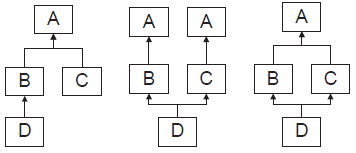
\includegraphics[width=0.47\textwidth]{Hierarchies.png}
  \caption{Single inheritance, repeated multiple inheritance and virtual multiple inheritance}
  \label{fig:hierarchy}
\end{figure}

\noindent
Note that the above picture portrais subobject relatedion, not the inheritance.

Figure~\ref{fig:objlayout} shows a typical object layout generated by a \Cpp{} 
compiler for class \code{D} from Figure~\ref{fig:inheritance}(1) under repeated 
(1) and virtual (2) inheritance of \code{A}. The layouts represent an encoding 
of the corresponding subobject graphs from Figures \ref{fig:inheritance}(2a) and 
\ref{fig:inheritance}(2b) respectively.

\begin{figure}[htbp]
  \centering
    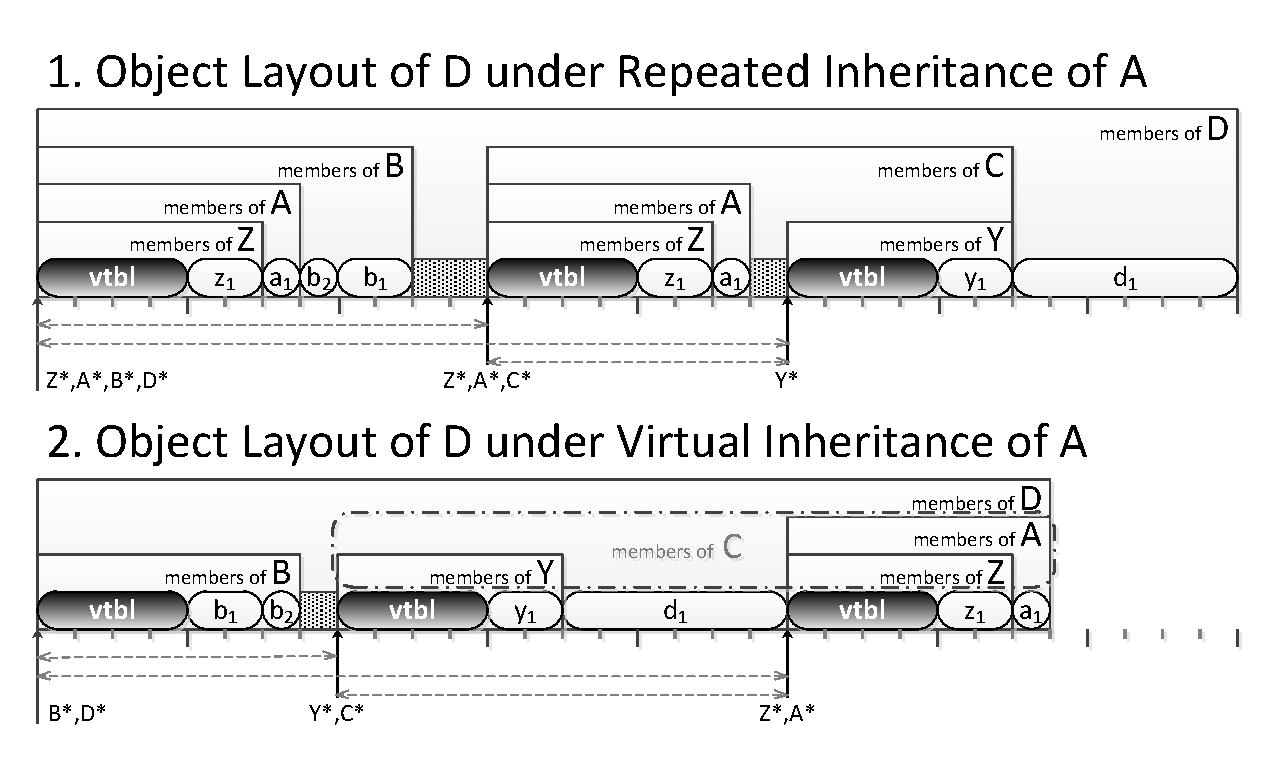
\includegraphics[width=0.47\textwidth]{obj-layout.pdf}
  \caption{Object Layout under Multiple Inheritance}
  \label{fig:objlayout}
\end{figure}

Due to the extensibility of classes, the layout decisions for classes must be 
made independently of their derived classes -- a property of the \Cpp{} object 
model that we will refer to as \emph{layout independence}. In turn, the layout of derived   
classes must conform to the layout of their base classes relatively to the offset 
of the base class within the derived one. For example, the layout of \code{A} in 
\code{C} is exactly the same as the layout of \code{A} in \code{B} and is simply
the layout of \code{A}. Base classes inherited virtually do not contribute to 
the fixed layout because they are looked up indirectly at run-time; however, 
they are not exempt from layout independence, since their lookup rules are 
agnostic of the concrete dynamic type.
%Because of this indirection, the use of virtual inheritance incures slight 
%overhead at run-time. 

Under non-virtual inheritance, members of the base class are typically laid out 
before the members of derived class, resulting in the base class being at the 
same offset as the derived class itself. In our example, the offset of \code{A} 
in \code{B} under regular (non-virtual) inheritance of \code{A} is 0.
Under multiple inheritance, different base classes might be at different offsets 
in the derived class, which is why pointers of a given static type may be 
pointing only to certain subobjects in it. These positions are marked in the 
picture with vertical arrows decorated with the set of pointer types whose 
values may point into that position. Run-time conversions between such pointers 
represent casts between subobjects of the same dynamic type and may require 
adjustments to this-pointer (shown with dashed arrows) for type safety.

A class that declares or inherits a virtual function is called a 
\emph{polymorphic class}. The \Cpp{} standard~\cite{C++11} does not prescribe any 
specific implementation technique for virtual function dispatch.
However, in practice, all \Cpp{} compilers use a strategy based on so-called
virtual function tables (or vtables for short) for efficient dispatch. 
The vtable is part of the reification of a polymorphic class type.  
\Cpp{} compilers embed a pointer to a vtable (vtbl-pointer for short) in every object of
polymorphic class type (and thus every subobject of that type inside other 
classes due to layout independence). CFront, the first \Cpp{} compiler, puts the 
vtbl-pointer 
at the end of an object. The so-called ``common vendor \Cpp{} ABI''~\cite{C++ABI} requires the 
vtbl-pointer to be at offset 0 of an object. ~\footnote{The following compilers 
are known to comply with the \Cpp{} ABI: GCC (3.x and up); Clang and llvm-g++; 
Linux versions of Intel and HP compilers, and compilers from ARM. See 
http://morpher.com/documentation/articles/abi/ for details.}. 
We do not have 
access to the unpublished Microsoft ABI, but we have experimental evidence that 
their \Cpp{} compiler also puts the vtbl-pointer at the start of an object.

While the exact offset of the vtbl-pointer within the (sub)object is not important 
for this discussion, because of layout independence every (sub)object of a 
polymorphic type \code{S} will have a vtbl-pointer at a predefined offset. 
Such offset may be different for different static types \code{S}, in which case 
the compiler will know at which offset in type \code{S} the vtbl-pointer is 
located, but it will be the same within any subobject of a static type 
\code{S}. For a library implementation we assume the presence of a function 
\code{template <typename S> intptr_t vtbl(const S* s);} 
that returns the address of the virtual table corresponding to the subobject 
pointed to by \code{s}. Such a function can be trivially implemented for the 
common vendor \Cpp{} ABI, where the vtbl-pointer is always at offset 0:

\begin{lstlisting}
template <typename S> std::intptr_t vtbl(const S* s) {
    static_assert(std::is_polymorphic<S>::value, "error");
    return *reinterpret_cast<const std::intptr_t*>(s);
}
\end{lstlisting}

\noindent
Each of the \code{vtbl} fields shown in Figure~\ref{fig:objlayout} holds a 
vtbl-pointer referencing a group of virtual methods known in the object's static 
type. Figure~\ref{fig:vtbl}(1) shows a typical layout of virtual function tables 
together with objects it points to for classes \code{B} and \code{D}.

\noindent
\begin{figure}[htbp]
  \centering
    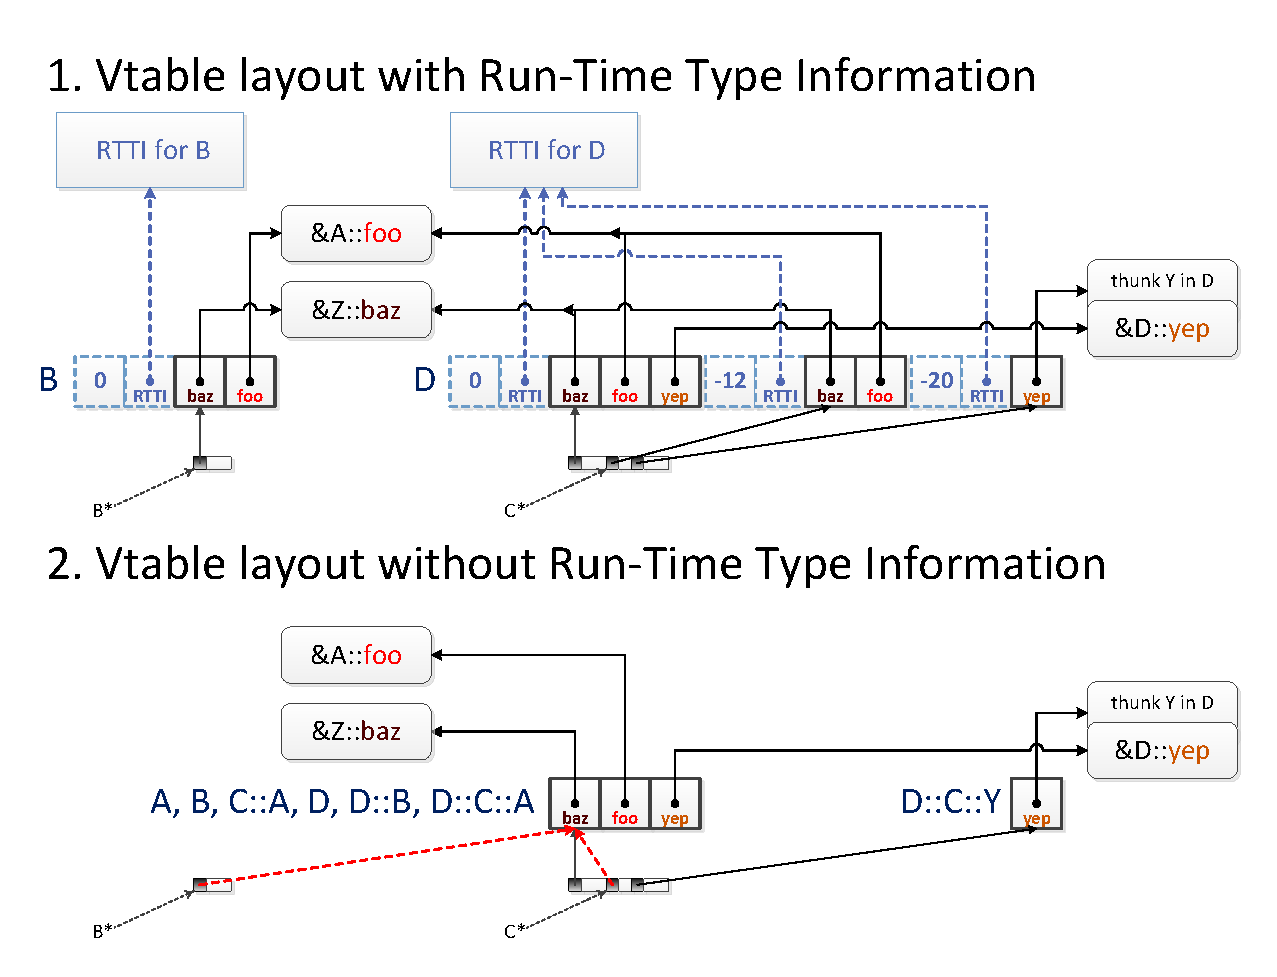
\includegraphics[width=0.49\textwidth]{v-table.pdf}
  \caption{VTable layout with and without RTTI}
  \label{fig:vtbl}
\end{figure}

Entries in the vtable to the right of the address pointed to by a vtbl-pointer 
represent pointers to functions, while entries to the left of it represent 
various additional fields like a pointer to a class' type information, offset to 
top, offsets to virtual base classes, etc. In many implementations, this-pointer 
adjustments required to dispatch properly the call were stored in the vtable 
along with function pointers. Today most implementations prefer to use 
\emph{thunks} or \emph{trampolines} -- additional entry points to a function, 
that adjust this-pointer before transferring the control to the function, -- 
which was shown to be more efficient~\cite{Driesen96}. Thunks in general may 
only be needed when virtual function is overridden. In such cases, the 
overridden function may be called via a pointer to a base class or a pointer to 
a derived class, which may not be at the same offset in the actual object.

The intuition behind our proposal is to use the values of vtbl-pointers stored 
inside the object to uniquely identify the subobject in it. There are several 
problems with the approach, however. First, the same vtbl-pointer is 
usually shared by multiple subobjects when one of them contains the other. For 
example, the first vtbl-pointer in Figure~\ref{fig:objlayout}(1) will be shared 
by objects of static type \code{Z*}, \code{A*}, \code{B*} and \code{D*}. This is 
not a problem for our purpose, because the subobjects of these types will be at 
the same offset in the object. Secondly, and more importantly, 
however, there are legitimate optimizations that let the compiler share the same 
vtable among multiple subobjects of often-unrelated types.

Generation of the \emph{Run-Time Type Information} (or RTTI for short) can 
typically be disabled with a compiler switch and the Figure~\ref{fig:vtbl}(2) 
shows the same vtable layouts once RTTI has been disabled. Since neither 
\code{baz} nor \code{foo} were overridden, the prefix of the vtable for the 
\code{C} subobject in \code{D} is exactly the same as the vtable for its 
\code{B} subobject, the \code{A} subobject of \code{C}, or the entire vtable of 
\code{A} and \code{B} classes. Such a layout, for example, is produced by 
Microsoft Visual \Cpp{} 11 when the command-line option \code{/GR-} is specified. 
The Visual \Cpp{} compiler has been known to unify code identical on binary level, 
which in some cases may result in sharing of the same vtable between unrelated 
classes (e.g. when virtual functions are empty).

%\Cpp{} supports multiple-inheritance of two kinds: repeated and virtual (shared). 
%\emph{Repeated inheritance} creates multiple independent subobjects of the same 
%type within the dynamic type. \emph{Virtual inheritance} creates only one 
%shared subobject, regardless of the inheritance paths. Consequently,
%it is not sufficient to talk only about the 
%static and dynamic types of an object -- one has to talk about a 
%\emph{subobject} of a certain static type accessible through a given inheritance 
%path within a dynamic type. 

We now would like to show more formally that in the presence of RTTI, a common vendor \Cpp{} ABI 
compliant implementation would always have all the vtbl-pointers different. To do 
so, we need a closer look at the notion of subobject, which has been formalized 
before~\cite{RF95,WNST06,RDL11}. We follow here the presentation of Ramamanandro 
et al~\cite{RDL11}.

\subsection{Subobjects}
\label{sec:subobj}

We assume a program $\mathfrak{P}$ is represented by its class table, which can be 
queried for inheritance relations between classes. All subsequent definitions 
are implicitly parameterized over a given program $\mathfrak{P}$. 
A class $B$ is a \emph{direct repeated base class} of  
$D$ if $B$ is mentioned in the list of base classes of $D$ without the 
\code{virtual} keyword ($D \prec_R B$). Similarly, a class $B$ is a \emph{direct 
shared base class} of $D$ if $B$ is mentioned in the list of base classes of $D$ 
with the \code{virtual} keyword ($D \prec_S B$). A reflexive transitive closure 
of these relationships $\preceq^*=(\prec_R \cup \prec_S)^*$ defines the 
\emph{subtyping} relation on types of program $\mathfrak{P}$.
A base class \emph{subobject} of a given \emph{complete object} is represented by a pair 
$\sigma = (h,l)$ with $h \in \{\mathsf{Repeated},\mathsf{Shared}\}$ representing the 
kind of inheritance (single inheritance is $\mathsf{Repeated}$ with one base class) and $l$ 
representing the path in a non-virtual inheritance graph.
A judgment of the form $\mathfrak{P}\vdash C\leftY\sigma\rightY A$ states that 
in a program $\mathfrak{P}$, $\sigma$ designates a subobject of static type $A$ 
within an object of type $C$. Omitting the context $\mathfrak{P}$: 

A predicate $C\leftY\sigma\rightY A$ they introduce means that $\sigma$ 
designates a subobject of static type $A$ within the most derived object of 
type $C$.

\begin{mathpar}
\inferrule
{C \prec_S B \\ B\leftY(h,l)\rightY A}
{C\leftY(\mathsf{Shared},l)\rightY A}

\inferrule
{}
{C\leftY(\mathsf{Repeated},C::\epsilon)\rightY C}

\inferrule
{C \prec_R B \\ B\leftY(\mathsf{Repeated},l)\rightY A}
{C\leftY(\mathsf{Repeated},C::l)\rightY A}
\end{mathpar}

\noindent
$\epsilon$ indicates an empty path, but we will generally omit it in writing 
when understood from the context. In the case of repeated inheritance in 
Figure~\ref{fig:inheritance}(1), an object of the dynamic class \code{D} 
will have the following $\mathsf{Repeated}$ subobjects:
\code{D::C::Y}, 
\code{D::B::A::Z}, 
\code{D::C::A::Z}, 
\code{D::B::A}, 
\code{D::C::A}, 
\code{D::B}, 
\code{D::C}, 
\code{D}.
Similarly, in case of virtual inheritance in the same example, an object of the 
dynamic class \code{D} will have the following $\mathsf{Repeated}$ subobjects:
\code{D::C::Y}, 
\code{D::B}, 
\code{D::C}, 
\code{D}
as well as the following $\mathsf{Shared}$ subobjects: 
\code{D::A::Z}, 
\code{D::Z}, 
\code{D::A}. See Figure~\ref{fig:inheritance} for illustration.

It is easy to show by structural induction on the above definition, that 
$C\leftY\sigma\rightY A \implies \sigma=(h,C::l_1) \wedge \sigma=(h,l_2::A::\epsilon)$, 
which simply means that any path to a subobject of static type $A$ within the 
object of dynamic type $C$ starts with $C$ and ends with $A$. This 
observation shows that $\sigma_\bot = (\mathsf{Shared},\epsilon)$ does not 
represent a valid subobject. If $\Sigma_\mathfrak{P}$ is the domain of all subobjects in 
the program $\mathfrak{P}$ extended with $\sigma_\bot$, then a \emph{cast} operation can be 
understood as a function $\delta : \Sigma_\mathfrak{P} \rightarrow \Sigma_\mathfrak{P}$. We use 
$\sigma_\bot$ to indicate an impossibility of a cast. The fact that $\delta$ is 
defined on subobjects as opposed to actual run-time values reflects the 
non-coercive nature of the operation, i.e. the underlying value remains the 
same. Any implementation of such a function must thus satisfy the following 
condition:
\begin{eqnarray*}
C \leftY\sigma_1\rightY A \wedge \delta(\sigma_1) = \sigma_2 \implies C \leftY\sigma_2\rightY B
\end{eqnarray*}
\noindent
i.e. the dynamic type of the value does not change during casting, only the way 
we reference it does. Following the definitions from 
\textsection\ref{sec:specifics}, $A$ is the \emph{source type} and $\sigma_1$ is 
the \emph{source subobject} of the cast, while $B$ is the \emph{target type} and 
$\sigma_2$ is the \emph{target subobject} of it. The type $C$ is the 
dynamic type of the value being casted. The \Cpp{} semantics states more 
requirements to the implementation of $\delta$: e.g. 
$\delta(\sigma_\bot) = \sigma_\bot$ etc. but their precise modeling is out of 
scope of this discussion. We would only like to point out here that since 
the result of the cast does not depend on the actual value and only on the 
source subobject and the target type, we can memoize the outcome of a cast on 
one instance in order to apply its results to another.

%Figure~\ref{fig:objlayout}(1)
%$Z\leftY(\mathsf{Repeated},      [Z])\rightY Z$,
%$A\leftY(\mathsf{Repeated},    [A,Z])\rightY Z$,
%$B\leftY(\mathsf{Repeated},  [B,A,Z])\rightY Z$,
%$D\leftY(\mathsf{Repeated},[D,B,A,Z])\rightY Z$,
%$C\leftY(\mathsf{Repeated},  [C,A,Z])\rightY Z$,
%$D\leftY(\mathsf{Repeated},[D,C,A,Z])\rightY Z$,
%$Y\leftY(\mathsf{Repeated},      [Y])\rightY Y$,  
%$C\leftY(\mathsf{Repeated},    [C,Y])\rightY Y$,
%$D\leftY(\mathsf{Repeated},  [D,C,Y])\rightY Y$,
%$A\leftY(\mathsf{Repeated},      [A])\rightY A$, 
%$B\leftY(\mathsf{Repeated},    [B,A])\rightY A$,
%$D\leftY(\mathsf{Repeated},  [D,B,A])\rightY A$,
%$C\leftY(\mathsf{Repeated},    [C,A])\rightY A$,
%$D\leftY(\mathsf{Repeated},  [D,C,A])\rightY A$,
%$B\leftY(\mathsf{Repeated},      [B])\rightY B$,
%$D\leftY(\mathsf{Repeated},    [D,B])\rightY B$,
%$C\leftY(\mathsf{Repeated},      [C])\rightY C$,
%$D\leftY(\mathsf{Repeated},    [D,C])\rightY C$,
%$D\leftY(\mathsf{Repeated},      [D])\rightY D$,
%
%Figure~\ref{fig:objlayout}(2)
%$Z\leftY(\mathsf{Repeated},      [Z])\rightY Z$,
%$A\leftY(\mathsf{Repeated},    [A,Z])\rightY Z$,
%$B\leftY(\mathsf{Shared},    [B,A,Z])\rightY Z$,
%$C\leftY(\mathsf{Shared},    [C,A,Z])\rightY Z$,
%$D\leftY(\mathsf{Shared},    [D,A,Z])\rightY Z$,
%$D\leftY(\mathsf{Shared},      [D,Z])\rightY Z$,
%$Y\leftY(\mathsf{Repeated},      [Y])\rightY Y$,  
%$C\leftY(\mathsf{Repeated},    [C,Y])\rightY Y$,
%$D\leftY(\mathsf{Repeated},  [D,C,Y])\rightY Y$,
%$A\leftY(\mathsf{Repeated},      [A])\rightY A$, 
%$B\leftY(\mathsf{Shared},      [B,A])\rightY A$,
%$C\leftY(\mathsf{Shared},      [C,A])\rightY A$,
%$D\leftY(\mathsf{Shared},      [D,A])\rightY A$,
%$B\leftY(\mathsf{Repeated},      [B])\rightY B$,
%$D\leftY(\mathsf{Repeated},    [D,B])\rightY B$,
%$C\leftY(\mathsf{Repeated},      [C])\rightY C$,
%$D\leftY(\mathsf{Repeated},    [D,C])\rightY C$,
%$D\leftY(\mathsf{Repeated},      [D])\rightY D$,

\subsection{Uniqueness of vtbl-pointers under common ABI}
\label{sec:uniq}

A class that declares or inherits a virtual function is called a 
\emph{polymorphic class}~\cite[\textsection 10.3]{C++0x}. The C++ ABI in turn defines 
\emph{dynamic class} to be a class requiring a virtual table pointer (because it 
or its bases have one or more virtual member functions or virtual base classes). 
A polymorphic class is thus a dynamic class by definition.

A \emph{virtual table pointer} (vtbl-pointer) is a member of object's layout 
pointing to a virtual table. A \emph{virtual table} is a table of information used 
to dispatch virtual functions, access virtual base class subobjects, and to 
access information for \emph{RunTime Type Identification} (RTTI). Because of repeated
inheritance, an object of given type may have several vtbl-pointers in it. Each 
such pointer corresponds to one of the polymorphic base classes. Given an object 
$a$ of static type $A$ that has $k$ vtbl-pointers in it, we will use the same 
notation we use for regular fields to refer them: $a.\textit{vtbl}_i$.

A \emph{primary base class} for a dynamic class is the unique base class (if any) 
with which it shares the virtual table pointer at offset 0. The data layout 
procedure for non-POD types described in \textsection2.4 of the C++ ABI~\cite{C++ABI} 
requires dynamic classes either to allocate vtable pointer at offset 0 or share 
the virtual table pointer from its primary base class, which is by definition at 
offset 0. For our purpose this means that we can rely on a virtual table pointer 
always being present at offset 0 for all dynamic classes, and thus for all polymorphic 
classes.

\begin{lemma}
In an object layout that adheres to the C++ ABI, a polymorphic class always has a 
virtual table pointer at offset 0.
\label{lem:vtbl}
\end{lemma}

\noindent
Knowing how to extract a vtbl-pointer as well as that all the objects of the 
same most derived type share the same vtbl-pointers, the idea is to use their 
values to uniquely identify the type and subobject within it. Unfortunately 
nothing in the C++ ABI states these pointers should be unique. A popular 
optimization technique lets the compiler share the virtual table of a derived 
class with its primary base class as long as the derived class that does not 
override any virtual methods. Use of such optimization will violate the 
uniqueness of vtbl-pointers; however, we show below that in the presense of 
RTTI, a C++ ABI-compliant implementation is guaranteed to have different values 
of vtbl-pointers in different subobjects.

%C++ standard requires an argument of \code{dynamic_cast} to be a pointer to or 
%an lvalue of a polymorphic type when performing \emph{downcast} -- a cast from 
%base to derived~\cite[\textsection 5.2.7-6]{C++0x}. We can thus always safely 
%extract virtual table pointer from offset 0 of any valid argument to 
%\code{dynamic_cast}.

%Similarly, each class that has virtual member functions or virtual bases has an 
%associated set of virtual tables. There may be multiple virtual tables for a 
%particular class, if it is used as a base class for other classes. However, the 
%virtual table pointers within all the objects (instances) of a particular 
%most-derived class point to the same set of virtual tables.

The exact content of the virtual table is not important for our discussion, but 
we would like to point out a few fields in it. The following definitions are 
copied verbatim from the C++ ABI~\cite[\textsection 2.5.2]{C++ABI}:

\begin{itemize}
\setlength{\itemsep}{0pt}
\setlength{\parskip}{0pt}
\item The \emph{typeinfo pointer} points to the typeinfo object used for RTTI. 
      It is always present.  
\item The \emph{offset to top} holds the displacement to the top of the object 
      from the location within the object of the virtual table pointer that 
      addresses this virtual table, as a \code{ptrdiff_t}. It is always present.
\item \emph{Virtual Base (vbase) offsets} are used to access the virtual bases 
      of an object. Such an entry is added to the derived class object address 
      (i.e. the address of its virtual table pointer) to get the address of a 
      virtual base class subobject. Such an entry is required for each virtual 
      base class.
\end{itemize}

\noindent
Given a virtual table pointer \code{vtbl}, we will refer to these fields as 
\code{rtti(vtbl)}, \code{off2top(vtbl)} and \code{vbase(vtbl)} respectively. 
We will also assume presence of a function $\mathit{offset}(\sigma)$ that defines the 
offset of the base class identified by the end of the path $\sigma$ within a 
class identified by its first element.

\begin{theorem}
In an object layout that adheres to the C++ ABI with present runtime type 
information, the equality of virtual table pointers of two objects of the same 
static type implies that they both belong to subobjects with the same 
inheritance path in the same most-derived type.
\begin{eqnarray*}
    \forall a_1, a_2 : A\ |\ a_1\in C_1\leftY\sigma_1\rightY A \wedge a_2\in C_2\leftY\sigma_2\rightY A \\
    a_1.\textit{vtbl}_i = a_2.\textit{vtbl}_i \Rightarrow C_1 = C_2 \wedge \sigma_1 = \sigma_2
\end{eqnarray*}
\label{thm:vtbl}
\end{theorem}
\begin{proof}
Let us assume first $a_1.\textit{vtbl}_i = a_2.\textit{vtbl}_i$ but $C_1 \neq C_2$. In this case we 
have \code{rtti}$(a_1.\textit{vtbl}_i) = $\code{rtti}$(a_2.\textit{vtbl}_i)$. By definition 
\code{rtti}$(a_1.\textit{vtbl}_i) = C_1$ while \code{rtti}$(a_2.\textit{vtbl}_i) = C_2$, which 
contradicts that $C_1 \neq C_2$. Thus $C_1 = C_2 = C$.

Let us assume now that $a_1.\textit{vtbl}_i = a_2.\textit{vtbl}_i$ but $\sigma_1 \neq \sigma_2$. 
Let $\sigma_i=\langle h_i,l_i\rangle,i=1,2$ 

If $h_1 \neq h_2$ then one of them refers to a virtual base while the other to a 
repeated one. Assuming $h_1$ refers to a virtual path, \code{vbase}$(a_1.\textit{vtbl}_i)$ 
has to be defined inside the vtable according to the ABI, while 
\code{vbase}$(a_2.\textit{vtbl}_i)$ -- should not. This would contradict again that both 
$vtbl_i$ refer to the same virtual table.

We thus have $h_1 = h_2 = h$. If $h = \mathrm{Shared}$ then there is only one path to 
such $A$ in $C$, which would contradict $\sigma_1 \neq \sigma_2$. 
If $h = \mathrm{Repeated}$ then we must have that $l_1 \neq l_2$. In this case let $k$ be 
the first position in which they differ: 
$l_1^j=l_2^j \forall j<k \wedge l_1^k\neq l_2^k$. Since our class $A$ is a base 
class for classes $l_1^k$ and $l_2^k$, both of which are in turn base classes of 
$C$, the object identity requirement of C++ requires that the relevant subobjects 
of type $A$ have different offsets within class $C$: 
$\mathit{offset}(\sigma_1)\neq \mathit{offset}(\sigma_2)$ However 
$\mathit{offset}(\sigma_1)=$\code{off2top}$(a_1.\textit{vtbl}_i)=$\code{off2top}$(a_2.\textit{vtbl}_i)=\mathit{offset}(\sigma_2)$ 
since $a_1.\textit{vtbl}_i = a_2.\textit{vtbl}_i$, which contradicts that the offsets are different.
\end{proof}

\noindent
Conjecture in the other direction is not true in general as there may be 
duplicate virtual tables for the same type present at run-time. This happens in 
many C++ implementations in the presence of DLLs as the same class compiled into 
executable and into a DLL it loads may have identical virtual tables inside the 
executable's and DLL's binaries.

Note also that we require both static types to be the same. Dropping this 
requirement and saying that equality of vtbl-pointers also implies equality of 
the static types is not true in general because a derived class will share the 
vtbl-pointer with its primary base class (see Lemma~\ref{lem:vtbl}). The theorem 
can be reformulated, however, stating that one static type will necessarily have 
to be a subtype of the other. The current formulation is sufficient for our 
purposes, while reformulation would have required more elaborate discussion of 
the algebra of subobjects~\cite{RDL11}, which we touch only briefly.

\begin{corollary}
Results of \code{dynamic_cast} can be reapplied to a different instance from 
within the same subobject. 

$\forall A,B \forall a_1, a_2 : A\ |\ a_1.\textit{vtbl}_i = a_2.\textit{vtbl}_i \Rightarrow$ \\
\code{dynamic_cast<B>}$(a_1).\textit{vtbl}_j = $\code{dynamic_cast<B>}$(a_2).\textit{vtbl}_j \vee$ \\
\code{dynamic_cast<B>}$(a_1)$ throws $\wedge$ \code{dynamic_cast<B>}$(a_2)$ throws.
\label{crl:vtbl}
\end{corollary}

\noindent
During construction and deconstruction of 
an object, the value of a given vtbl-pointer may change. In particular, 
that value will reflect the fact that the dynamic type of the object is the type of its 
fully constructed part only. This does not affect our reasoning, as during 
such transition we also treat the object to have the type of its fully 
constructed base only. Such interpretation is in line with the \Cpp{} semantics for 
virtual function calls and the use of RTTI during construction and destruction of an 
object. Once the complete object is fully constructed, the value of the 
vtbl-pointer will remain the same for the lifetime of the object.

\subsection{Vtable Pointer Memoization}
\label{sec:vtblmem}

The memoization device can almost immediately be used for multi-way type testing by 
using \code{dynamic_cast<Ti>} as a predicate $P_i$. This cannot be considered a 
type switching solution, however, as one would expect to also have a reference 
to the uncovered type. Using a \code{static_cast<Ti>} upon successful type test 
would have been a solution if we did not have multiple inheritance. It certainly 
can be used as such in languages with only single inheritance. For the fully 
functional \Cpp{} solution, we combine the memoization device with the properties 
of virtual table pointers into a \emph{Vtable Pointer Memoization} technique.

The \Cpp{} standard implies that information about types is available at run time 
for three distinct purposes~\cite[\textsection 2.9.1]{C++ABI}:

\begin{itemize}
\setlength{\itemsep}{0pt}
\setlength{\parskip}{0pt}
\item to support the \code{typeid} operator,
\item to match an exception handler with a thrown object, and
\item to implement the \code{dynamic_cast} operator.
\end{itemize}

\noindent
and if any of these facilities are used in a program that was compiled with 
RTTI disabled, the compiler shall emit a warning. Some 
compilers (e.g. Visual \Cpp{}) additionally let a library check presence of RTTI 
through a predefined macro, thus letting it report an error if its dependence on 
RTTI cannot be satisfied. Since our solution depends on \code{dynamic_cast}% to perform casts at run-time
, according to the third requirement we implicitly rely on the presence of RTTI and thus 
fall into the setting that guarantees the preconditions of Theorem~\ref{thm:vtbl}.
Besides, all the objects that will be coming through a particular type switch will 
have the same static type, and thus the theorem guarantees that different vtbl-pointers 
will correspond to different subobjects. The idea is thus to group them 
according to the value of their vtbl-pointer and associate both jump target 
and the required offset through the memoization device:

\begin{lstlisting}
typedef pair<ptrdiff_t,size_t> target_info; //(offset,target)
static unordered_map<intptr_t, target_info> jump_targets;
      auto*  sptr = &x; // name to access subject
const void*       tptr; 
target_info& info = jump_targets[vtbl(sptr)];
switch (info.second) {{ default: 
\end{lstlisting}

\noindent
We use the virtual table pointer extracted from a polymorphic object pointed to 
by \code{p} as a key for association. The value stored along the key in 
association now keeps both: the target for the switch as well as a memoized 
offset for dynamic cast. 

The code for the $i^{th}$ case now evaluates the required offset on the first 
entry and associates it and the target with the vtbl-pointer of the subject.
The call to \code{adjust_ptr<Ti>} re-establishes the invariant that 
\code{match} is a reference to type \code{Ti} of the subject \code{x}.
%The condition of the inner if-statement is only needed to implement the 
%sequential all-fit semantics and can be removed when fall-through behavior is 
%not required.

\begin{lstlisting}
  if (tptr = dynamic_cast<const Ti *>(sptr)) {
        if (info.second == 0) { // supports fall-through
      info.first  = intptr_t(tptr)-intptr_t(sptr); // offset
            info.second = @$i$@; // jump target
        }
  case @$i$@: // @$i$@ is a constant - clause's position in switch
    auto match = adjust_ptr<Ti>(sptr,info.first);
        si;
    }
\end{lstlisting}

\noindent
The main condition remains the same. We keep checking for the first initialization 
because we allow fall-through semantics here, letting the user break from the 
switch when needed. Upon first entry we compute the offset that the dynamic cast 
performed and save it together with target associated to the virtual table 
pointer. On the next iteration we will jump directly to the case label and 
restore the invariant of \code{matched} being a properly-casted reference to the 
derived object.

The use of dynamic cast makes a huge difference in comparison to the use of 
static cast we dismissed above. First of all the C++ type system is much more 
restrictive about the static cast and many cases where it is not allowed can 
still be handled by dynamic cast. Examples of these include downcasting from an 
ambiguous base class or cross-casting between unrelated base classes.

An important benefit we get from this optimization is that we do not store the 
actual values (pointers to objects) in the hash table anymore, but group them 
into equivalence classes based on their virtual table pointers. The number of 
such pointers in a program is always bound by $O(|A|)$, where $A$ represents the 
static type of an object, while $|A|$ represents the number of classes directly 
or indirectly derived from $A$. The linear coefficient hidden in big-o notation 
reflects possibly multiple vtbl-pointers in derived classes due to the use of 
multiple inheritance.

\begin{figure}[htbp]
  \centering
    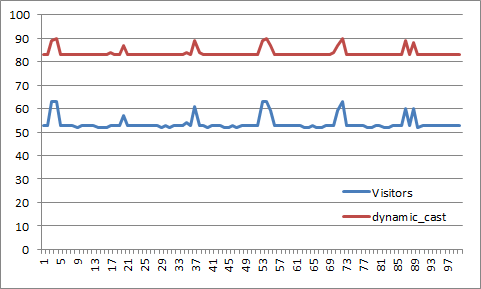
\includegraphics[width=0.47\textwidth]{DCast-vs-Visitors3.png}
  \caption{Time to uncover i\textsuperscript{th} case. X-axis - case i; Y-axis - cycles per iteration}
  \label{fig:DCastVis3}
\end{figure}

The most important benefit of this optimization, however, is the constant time 
on average used to dispatch each of the case clauses, regardless of their 
position in the type switch. The net effect of this optimization can be seen in Figure~\ref{fig:DCastVis3}. 
We can see that the time does not increase with the position of the case we are 
handling. The spikes represent activities on computer during measurement and are 
present in both measurements. 
The constant time on average comes from the average complexity 
of accessing an element in an \code{unordered_map}, while its worst complexity can 
be proportional to the size of the map. We show in the next section, however, 
that most of the time we will be bypassing traditional access to elements of the 
map, because, as-is, the type switch is still about 50\% slower than the visitor 
design pattern.

\noindent
Class \code{std::unordered_map} provides amortized constant time access on 
average and linear in the number of elements in the worst case. We show in the 
next section that most of the time we will be bypassing traditional access to 
its elements. We need this extra optimization because, as-is, the type switch is 
still about 50\% slower than the visitor design pattern.
\footnote{We are using 
speedups throughout the paper when comparing performance, so ``X is 42\% faster 
than Y'' or equally ``Y is 42\% slower than X'' means that Y's execution time is 
1.42 times X's execution time.}

Note that we can apply the reasoning of \textsection\ref{sec:memdev} and change 
the first-fit semantics of the resulting match statement into a best-fit 
semantics simply by changing the underlying cascading-if structure with decision 
tree. A compiler implementation of a type switch based on Vtable Pointer 
Memoization will certainly take advantage of this optimization to cut down the 
cost of the first run on a given vtbl-pointer, when the actual memoization happens.

Looking back at the example from \textsection\ref{sec:intro} and allowing for a few 
unimportant omissions, the first code snippet corresponds to what the macro 
\code{Match(x)} is expanded to when given a subject expression \code{x}. In order to 
see what \code{Case(Ti)} is expanded to, the second snippet has to be split on 
the line containing \code{si;} (excluding \code{si;} itself, which comes from 
source) and the second part (i.e. \} here) moved in front of the first one. The 
macro thus closes the scope of the previous case clause before starting the new 
one. \code{Case}'s expansion only relies on names introduced by \code{Match(x)}, 
its argument \code{Ti}, and a constant $i$, which can be generated from the
\code{__LINE__} macro, or, better yet, the \code{__COUNTER__} macro when 
supported by the compiler. The \code{EndMatch} macro simply closes the scopes 
(i.e. \}\} here). We refer the reader to the library source code for 
further details.

\subsubsection{Structure of Virtual Table Pointers}
\label{sec:sovtp}

Virtual table pointers are not entirely random addresses in memory and have 
certain structure when we look at groups of those that are associated with 
classes related by inheritance. Let us first look at some vtbl pointers that 
were present in some of our tests. The 32-bit pointers are shown in binary form 
(lower bits on the right) and are sorted in ascending order:

\begin{verbatim}
00000001001111100000011001001000
00000001001111100000011001011100
00000001001111100000011001110000
 ...
00000001001111100000011111011000
00000001001111100000011111101100
\end{verbatim}

Virtual table pointers are not constant values and are not even guaranteed to be 
the same between different runs of the same application. Techniques like 
\emph{address space layout randomization} or simple \emph{rebasing} of the entire 
module are likely to change these values. The relative distance between them is 
likely to remain the same though as long as they come from the same module.

Comparing all the vtbl pointers that are coming through a given match statement 
we can trace ar run time the set of bits in which they do and do not differ. 
For the above example it may look as \texttt{00000001001111100000X11XXXXXXX00} 
where positions marked with X represent bits that are different in some vtbl 
pointers.

When a DLL is loaded it may have its own copy of vtables for classes also used 
in other modules as well as vtables for classes it introduces. Comparing 
similarly all vtbl pointers coming only from this DLL we can get a different 
pattern \\ \texttt{01110011100000010111XXXXXXXXX000} and when compared over all 
the loaded modules the pattern will likely becomes something like 
\texttt{0XXX00X1X0XXXXXX0XXXXXXXXXXXXX00}.

The common bits on the right come from the virtual table size and alignment 
requirements, and, depending on compiler, configuration, and class hierarchy could 
easily vary from 2 to 6 bits. Because the vtbl-pointer under the C++ ABI points into 
an array of function pointers, the alignment requirement of 4 bytes for those 
pointers on a 32-bit architecture is what makes at least the last 2 bits to be 0. 
For our purpose the exact number of bits on the right is not important as we 
evaluate this number at run time based on vtbl-pointers seen so far. Here we only 
would like to point out that there would be some number of common bits on the 
right.

Another observation we made during our experiments with the vtbl-pointers of various 
existing applications was that the values of the pointers where changing more 
frequently in the lower bits than in the higher ones. We believe that this was 
happening because programmers tend to group multiple derived classes in the same 
translation unit so the compiler was emitting virtual tables for them close to 
each other as well. 

Note that derived classes that do not introduce their own virtual functions 
(even if they override some existing ones) are likely to have virtual tables of 
the same size as their base class. Even when they do add new virtual functions, 
the size of their virtual tables can only increase relative to their base 
classes. This is why the difference between many consecutive vtbl-pointers that 
came through a given match statement was usually constant or very slightly 
different.

The changes in higher bits were typically due to separate compilation and 
especially due to dynamically loaded modules. When a DLL is loaded, it may have 
its own copies of vtables for classes that are also used in other modules, in addition to 
vtables for classes it introduces. Comparing all vtbl-pointers coming only from 
that DLL we can get a different pattern \texttt{01110011100000010111XXXXXXXXX000} 
and when compared over all the loaded modules the pattern will likely become 
something like \texttt{0XXX00X1X0XXXXXX0XXXXXXXXXXXXX00}. Overall they were not 
changing the general tendency we saw: smaller bits were changing more frequently 
than larger ones, with the exception of the lowest common bits, of course.

These observations made virtual table pointers of classes related by inheritance 
ideally suitable for indexing -- the values obtained by throwing away the common 
bits on the right were compactly distributed in small disjoint ranges. We use 
those values to address a cache built on top of the hash table in order to 
eliminate a hash table lookup in most of the cases.  The important 
guarantee about the validity of the cached hash table references comes from the 
C++0x standard, which states that ``insert and emplace members shall not affect 
the validity of references to container elements''~\cite[\textsection 
23.2.5(13)]{C++0x}. 

Depending on the number of actual collisions that happen in the cache, our 
vtable pointer memoization technique can come close to, and even outperform, the 
visitor design pattern. The numbers are, of course, averaged over many runs as 
the first run on every vtbl-pointer will take an amount of time as shown in 
Figure\ref{fig:DCastVis1}. We did however test our technique on real code and 
can confirm that it does perform well in the real-world use cases.

The information about jump targets and necessary offsets is just an example of 
information we might want to be able to associate with, and access via, virtual 
table pointers. Our implementation of \code{memoized_cast} from 
\textsection\ref{sec:memcast} effectively reuses this general data structure with 
a different type of element values. We thus created a generic reusable class 
\code{vtblmap<T>} that maps vtbl-pointers to elements of type T. We will refer 
to the combined cache and hash-table data structure, extended with the logic for 
minimizing conflicts presented below, as a \emph{vtblmap} data structure.

\subsection{Minimization of Conflicts}
\label{sec:moc}

Virtual table pointers are not constant values and are not even guaranteed to be 
the same between different runs of the application, because techniques like 
\emph{address space layout randomization} or \emph{rebasing} of the module are 
likely to change them. The relative distance between them will remain the same 
as long as they come from the same module.

Knowing that vtbl-pointers point into an array of function pointers, we should 
expect them to be aligned accordingly and thus have a few lowest bits as zero. 
Moreover, since many derived classes do not introduce new virtual functions, 
the size of their virtual tables remains the same. When allocated sequentially 
in memory, we can expect a certain number of lowest bits in the vtbl-pointers 
pointing to them to be the same.
These assumptions, supported by actual observations, made virtual table 
pointers of classes related by inheritance ideally suitable for hashing: the 
values obtained by throwing away the common bits on the right were compactly 
distributed in small disjoint ranges (\textsection\ref{sec:hierarchies}). We use 
them to address a cache built on top of the hash table in order to eliminate a 
hash table lookup in most of the cases.

Let $\Xi$ be the domain of integral representations of pointers. Given a cache 
with $2^k$ entries, we use a family of hash functions $H_{kl} : \Xi \rightarrow [0..2^k-1]$ 
defined as $H_{kl}(v)=v/2^l \mod 2^k$ to index the cache, where $l \in [0..32]$ 
(assuming 32 bit addresses) is a parameter modeling the number of common bits on 
the right. Division and modulo are implemented with bit operations since the
denominator in each case is a power of 2, which in turn explains the choice of 
the cache size.

Given a hash function $H_{kl}$, pointers $v'$ and $v''$ are said to be in 
\emph{conflict} when $H_{kl}(v')=H_{kl}(v'')$. For a given set of pointers 
$V \in 2^{\Xi}$, we can always find such $k$ and $l$ that $H_{kl}$ will render no  
conflicts between its elements, but the required cache size $2^k$ can be too 
large to justify the use of memory. The value $K$ such that $2^{K-1} < |V| \leq 2^K$ 
is the smallest value of $k$ under which absence of conflicts is still possible. 
We thus allow $k$ to vary only in the range $[K,K+1]$ to ensure that the cache size 
is never more than 4 times bigger than the minimum required cache size.

Given a set $V = \{v_1, ... , v_n\}$, we would like to find a pair of parameters 
$(k,l)$ such that $H_{kl}$ will render the least number of conflicts on the 
elements of $V$. Since for a fixed set $V$, parameters $k$ and $l$ vary in a 
finite range, we can always find the optimal $(k,l)$ by trying all the
combinations. Let $H_{kl}^V : V \rightarrow [0..2^k-1]$ be the hash function 
corresponding to such optimal $(k,l)$ for the set $V$. 

In our setting, the set $V$ represents the set of vtbl-pointers coming through a 
particular type switch. While the exact values of these pointers are not known 
until run-time, their offsets from the module's base address are. This is generally 
sufficient to estimate optimal $k$ and $l$ in a compiler setting. In the library 
setting, we recompute them after a given number of actual collisions in cache.

When $H_{kl}^V$ is injective (renders 0 conflicts on $V$), the frequency of any 
given vtbl-pointer $v_i$ coming through the type switch does not affect the 
overall performance of the switch. However when $H_{kl}^V$ is not injective, we 
would prefer the conflict to happen on less frequent vtbl-pointers.
Given a probability $p(v_i)$ of each vtbl-pointer $v_i \in V$ we can compute the 
probability of conflict rendered by a given $H_{kl}$:

\begin{eqnarray*}
p_{kl}(V)=\sum\limits_{j=0}^{2^k-1}\of{\sum\limits_{v_{i} \in V^j_{kl}}p(v_i)}\of{1-\frac{\sum\limits_{v_i \in V^j_{kl}}p(v_i)^2}{\of{\sum\limits_{v_{i} \in V^j_{kl}}p(v_i)}^2}}
\end{eqnarray*}

\noindent 
where $V^j_{kl}=\{v \in V | H_{kl}(v)=j\}$. In this case, the optimal hash 
function $H_{kl}^V$ can similarly be defined as $H_{kl}$ that minimizes the 
above probability of conflict on $V$.

The probabilities $p(v_i)$ can be estimated in a compiler setting through profiling, 
while in a library setting we let the user enable tracing of frequencies of 
each vtbl-pointer. This introduces an overhead of an increment into the critical 
path of execution, and according to our tests degrades the performance by 1-2\%. 
This should not be a problem as long as the overall performance gains from a
smaller probability of conflicts happening at run time. Unfortunately, in our 
tests the significant drop in the number of actual collisions was not reflected 
in a noticeable decrease in execution time, which is why we do not enable 
frequency tracing by default. As we will see in \textsection\ref{sec:hierarchies}, 
this was because the hash function $H_{kl}^V$ renders no conflicts on 
vtbl-pointers in most cases and the few collisions we were getting before 
inferring the optimal $k$ and $l$ even in non-frequency-based caching where 
incomparably smaller than the number of successful cache hits.

Assuming uniform distribution of $v_i$ in $V$ and substituting the probability 
$p(v_i)=\frac{1}{n}$, where $n=|V|$, into the above formula we get:

\begin{eqnarray*}
p_{kl}(V)=\sum\limits_{j=0}^{2^k-1}[|V^j_{kl}| \neq 0]\frac{|V^j_{kl}|-1}{n}
\end{eqnarray*}

\noindent
We use the Iverson bracket $[\pi]$ here to refer to the outcome of a predicate $\pi$ as numbers $0$ or $1$.
The value $|V^j_{kl}|$ represents the number of vtbl-pointers $v_i \in V$ that are mapped to the same location $j$ in cache with $H_{kl}^V$. Only 
one such vtbl-pointer will actually be present in that cache location at any given 
time, which is why the value $|V^j_{kl}|-1$ represents the number of ``extra'' 
pointers mapped into the entry $j$ on which a collision will happen. The overall 
probability of conflict thus only depends on the total number of these ``extra'' 
or conflicting vtbl-pointers. The $H_{kl}^V$ obtained by minimization of 
probability of conflict under uniform distribution of $v_i$ in $V$ is thus the 
same as the original $H_{kl}^V$ that was minimizing the number of conflicts. An 
important observation here is that since the exact location of these ``extra'' 
vtbl-pointers is not important and only the total number $m$ is, the probability 
of conflict under uniform distribution of $v_i$ in $V$ is always going to be of 
the discrete form $\frac{m}{n}$, where $0 \le m < n$.

%Depending on the number of actual collisions that happen in the cache, our 
%vtable pointer memoization technique can come close to, and even outperform, the 
%visitor design pattern. The numbers are, of course, averaged over many runs as 
%the first run on every vtbl-pointer will take an amount of time as shown in 
%Figure\ref{fig:DCastVis1}. We did however test our technique on real code and 
%can confirm that it does perform well in the real-world use cases.

%The information about jump targets and necessary offsets is just an example of 
%information we might want to be able to associate with, and access via, virtual 
%table pointers. Our implementation of \code{memoized_cast}~\cite[\textsection 9]{TR}, for example, 
%effectively reuses this general data structure with a different type of element 
%values. We thus created a generic reusable class \code{vtblmap<T>} that maps 
%vtbl-pointers to elements of type T. We will refer to the combined cache and 
%hash-table data structure, extended with the logic for minimizing conflicts 
%presented below, as a \emph{vtblmap} data structure.

%\subsubsection{Minimization of Conflicts}
%\label{sec:moc}

The small number of cycles that the visitor design pattern needs to uncover a 
type does not let us put too sophisticated cache indexing mechanisms into the 
critical path of execution. This is why we limit our indexing function to shifts 
and masking operations as well as choose the size of the cache to be a power of 2.

Throughout this section by \emph{collision} we will call a run-time condition in 
which the cache entry of an incoming vtbl pointer is occupied by another vtbl-pointer.
Collision requires vtblmap to fetch the data associated with the new 
vtbl-pointer from a slower hash-table and, under certain conditions, reconfigure 
cache for better performance. By \emph{conflict} we will call a different 
run-time condition under which given cache configuration maps two or more vtbl 
pointers to the same cache location. Presence of conflict does not necessarily 
imply presence of collisions, but collisions can only happen when there is a 
conflict. In the rest of this section we devise a mechanism that tries to 
minimize the amount of conflicts in a hope that it will also decrease the amount 
of actual collisions.

Given $n$ vtbl-pointers we can always find a cache size that will render no 
conflicts between them. The necessary size of such a cache, however, can be too 
big to justify the use of memory. This is why, in our current implementation, we 
always consider only 2 different cache sizes: $2^k$ and $2^{k+1}$ where 
$2^{k-1} < n \leq 2^k$. This guarantees that the cache size is never more than 4 
times bigger than the minimum required cache size.

During our experiments, we noticed that often the change in the smallest 
different bit happens only in a few vtbl-pointers, which was effectively 
cutting the available cache space in half. To overcome this problem, we let the 
number of bits by which we shift the vtbl-pointer vary further and compute it in 
a way that minimizes the number of conflicts.

To avoid doing any computations in the critical path, \code{vtblmap} only 
recomputes the optimal shift and the size of the cache when an actual collision 
happens. In order to avoid constant recomputations when conflicts are unavoidable, 
we add an additional restriction of only reconfiguring the optimal parameters if 
the number of vtbl-pointers in the \code{vtblmap} has increased since the last 
recomputation. Since the number of vtbl-pointers is of the order $O(|A|)$, where 
$A$ is the static type of all vtbl-pointers coming through a \code{vtblmap}, the 
restriction assures that reconfigurations will not happen infinitely often.

To minimize the number of recomputations even further, our library communicates 
to the \code{vtblmap}, through its constructor, the number of case clauses in 
the underlying match statement. We use this number as an estimate of the expected 
size of the \code{vtblmap} and pre-allocate the cache according to this estimated 
number. The cache is still allowed to grow based on the actual number of 
vtbl-pointers that comes through a \code{vtblmap}, but it never shrinks from the
initial value. This improvement significantly minimizes the number of collisions 
at early stages, as well as the number of possibilities we have to consider 
during reconfiguration.

The above logic of \code{vtblmap} always chooses the configuration that renders 
no conflicts, when such a configuration is possible during recomputation of 
optimal parameters. When this is not possible, it is natural to prefer collisions 
to happen on less-frequent vtbl-pointers.

We studied the frequency of vtbl-pointers that come through various match statements
of a C++ pretty-printer that we implemented on top of the Pivot 
framework~\cite{Pivot09} using our pattern-matching library. We ran the 
pretty-printer on a set of C++ standard library headers and then ranked all the  
classes from the most-frequent to the least-frequent ones, on average. The 
resulting probability distribution is shown with a thicker line in 
Figure\ref{fig:PowerLaw}.

\begin{figure}[htbp]
  \centering
    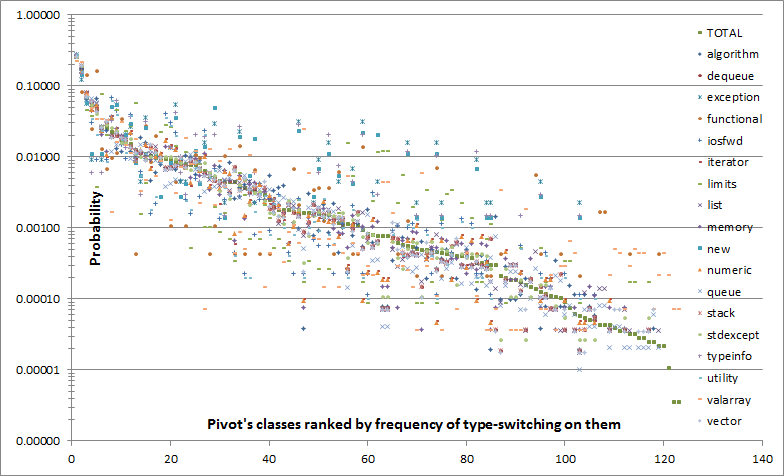
\includegraphics[width=0.47\textwidth]{std-lib-power-law-distributions.png}
  \caption{Probability distribution of various nodes in Pivot framework}
  \label{fig:PowerLaw}
\end{figure}

Note that Y-Axis is using logarithmic scale, suggesting that the resulting 
probability has power-law distribution. This is likely to be a specifics of our 
application, nevertheless, the above picture demonstrates that frequency of certain 
classes can be larger than the overall frequency of all the other classes. In 
our case, the two most frequent classes were representing the use of a variable in 
a program, and their combined frequency was larger than the frequency of all the 
other nodes. Naturally, we would like to avoid conflicts on such classes in the 
cache, when possible.

Let us assume that a given \code{vtblmap} contains a set of vtbl pointers 
$V = \{v_1, ... , v_n\}$ with known probabilities $p_i$ of occuring. For a cache 
of size $2^k$ and a shift by $l$ bits we get a cache-indexing function 
$f_{lk} : V \rightarrow [0..2^k-1]$ defined as $f_{lk}(v_i) = (v_i \gg l) \& (2^k-1)$.
To calculate the probability of conflict for a given $l$ and $k$ parameters, let 
us consider $j^{th}$ cache cell and a subset $V^j_{lk}=\{v \in V | f_{lk}(v)=j\}$. 
When the size of this subset $m=|V^j_{lk}|$ is greater than 1, we have a 
potential conflict as subsequent request for a vtbl pointer $v''$ might be 
different from the vtbl pointer $v'$ currenly stored in the cell $j$. Within the 
cell only the probability of not having a conflict is the probability of both 
values $v''$ and $v'$ be the same:
\begin{eqnarray*}
P(v''=v')=\sum\limits_{v_i \in V^j_{lk}}P(v''=v_i)P(v'=v_i)=\sum\limits_{v_i \in V^j_{lk}}P^2(v_i|V^j_{lk})=\\
=\sum\limits_{v_i \in V^j_{lk}}\frac{P^2(v_i)}{P^2(V^j_{lk})}=
\sum\limits_{v_i \in V^j_{lk}}\frac{p_i^2}{(\sum\limits_{v_{i'} \in V^j_{lk}}p_{i'})^2}=
\frac{\sum\limits_{v_i \in V^j_{lk}}p_i^2}{(\sum\limits_{v_{i} \in V^j_{lk}}p_{i})^2}
\end{eqnarray*}

The probability of having a conflict among the vtbl pointers of a given cell is 
thus one minus the above value:

\begin{eqnarray*}
P(v''\neq v')=1-\frac{\sum\limits_{v_i \in V^j_{lk}}p_i^2}{(\sum\limits_{v_{i} \in V^j_{lk}}p_{i})^2}
\end{eqnarray*}

To obtain probability of conflict given any vtbl pointer and not just the one 
from a given cell we need to sum up the above probabilities of conflict within a 
cell multiplied by the probability of vtbl pointer fall into that cell:

\begin{eqnarray*}
P_{lk}^{conflict}=\sum\limits_{j=0}^{2^k-1}P(V^j_{lk})(1-\frac{\sum\limits_{v_i \in V^j_{lk}}p_i^2}{(\sum\limits_{v_{i} \in V^j_{lk}}p_{i})^2})=\\
=\sum\limits_{j=0}^{2^k-1}(\sum\limits_{v_{i} \in V^j_{lk}}p_{i})(1-\frac{\sum\limits_{v_i \in V^j_{lk}}p_i^2}{(\sum\limits_{v_{i} \in V^j_{lk}}p_{i})^2})
\end{eqnarray*}

Our reconfiguration algorithm then iterates over possible values of $l$ and $k$ 
and chooses those that minimize the overal probability of conflict $P_{lk}^{conflict}$.
The only data still missing are the actual probabilities $p_i$ used by the above 
formula. They can be approximated in many different ways.

Besides probability distribution on all the tests, Figure~\ref{fig:PowerLaw} 
shows probabilities of a given node on each of the tests. The X-Axis in this 
case represents the ordering of all the nodes according to their overall rank 
of all the tests combined. As can be seen from the picture, the shape of each 
specific test's distribution still mimics the overal probability distribution. 
With this in mind we can simply let the user assign probabilities to each of the 
classes in the hierarchy and use these values during reconfiguration. The 
practical problem we came accross with this solution was that we wanted these 
probabilities be inheritable as Pivot separates interface and implementation 
classes and we prefered the user to define them on interfaces rather than on 
implementation classes. The easiest way to do so wast to write a dedicated 
function that would return the probabilities using a match statement. 
Unfortunately such a function will introduce a lot of overhead as it will 
ideally only be used very few times (since we try to minimize the amount of 
reconfiguration) and thus not be using memoized jumps but rather slow 
cascading-if.

A simpler and likely more precise way of estimating $p_i$ would be to count 
frequencies of each vtbl pointers directly inside the \code{vtblmap}. This 
introduces an overhead of an increment into the critical path of execution, but 
according to our tests was only degrading the overal performance by 1-2\%.
Instead, it was compensating with a smaller amount of conflicts and thus a 
potential gain of performance. We leave the choice of whether the library should 
count frequencies of each vtbl pointer to the user of the library as the 
concrete choice may be to advantage on some class hierarchies and to 
disadvantage on others.

Figure~\ref{fig:Collisions} compares the amount of collisions when frequency 
information is and is not used. The data was gathered from 312 tests on multiple 
match statements present in Pivot's C++ pretty printer when it was ran over 
standard library headers. In 122 of these test both schemes had 0 conflicts and 
these tests are thus not shown on the graph. The remaining tests where ranked by 
the amount of conflicts in the scheme that does not utilize frequency information.

\begin{figure}[htbp]
  \centering
    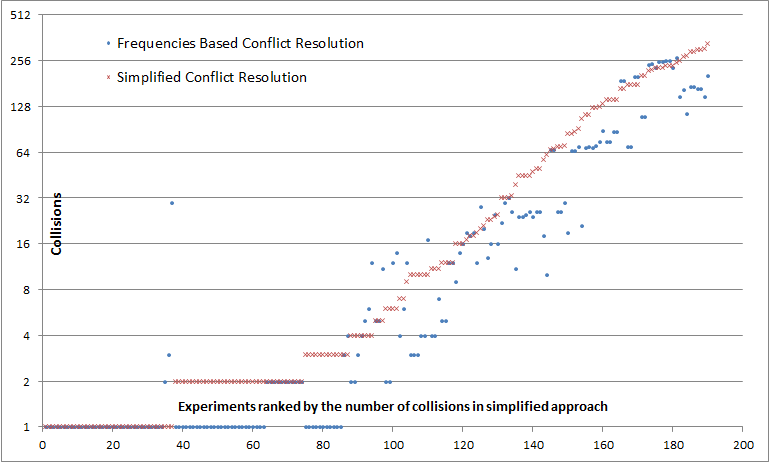
\includegraphics[width=0.47\textwidth]{CollisionsWithAndWithoutFrequencies.png}
  \caption{Decrease in number of collisions when probabilities of nodes are taken into account}
  \label{fig:Collisions}
\end{figure}

As can be seen from the graph, both schemes render quite low amount of 
collisions given that there was about 57000 calls in the rightmost test having 
the largest amount of conflicts. Taking into account that the Y-axis has 
logarithmic scale, the use of frequency information in many cases decreased the 
amount of conflicts by a factor of 2. The handfull of cases where the use of 
frequency increased the number of conflicts can be explained by the fact that 
the optimal values are not recomputed after each conflict, but after several 
conflicts and only if the amount of vtbl pointers in the vtblmap increased. These 
extra conditions sacrify optimality of parameters at any given time for the amount 
of times they are recomputed. By varying the number of conflicts we are willing 
to tolerate before reconfiguration we can decrease the number of conflicts by 
increasing the amount of recomputations and vise versa. From our experience, 
however, we saw that the drop in the number of conflicts was not translating 
into a proportional drop in execution time, while the amount of reconfigurations 
was proportional to the increase in execution time. This is why we choose to 
tolerate a relatively large amount of conflicts before recomputation just to 
keep the amount of recomputations low.

\section{(Ab)using Exceptions for Type Switching}
\label{sec:xpm}

Several authors had noted the relationship between exception handling and type 
switching before~\cite{Glew99,ML2000}. Not surprisingly, the exception handling 
mechanism of \Cpp{} can be abused to implement the first-fit semantics of a type 
switch statement. The idea is to harness the fact that catch-handlers in \Cpp{} 
essentially use first-fit semantics to decide which one is going to handle a 
given exception. The only problem is to raise an exception with a static type 
equal to the dynamic type of the subject.

To do this, we employ the \emph{polymorphic exception} idiom~\cite{PolyExcept} that 
introduces a virtual function \code{virtual void raise() const = 0;} into the 
base class, overridden by each derived class in syntactically the same way: 
\code{throw *this;}. The \code{Match}-statement then simply calls \code{raise} on its subject, 
while case clauses are turned into catch-handlers. The exact name of the 
function is not important, and is communicated to the library 
as \emph{raise selector} with \code{RS} specifier in the same way 
\emph{kind selector} and \emph{class members} are (\textsection\ref{sec:bnd}). 
The \code{raise} member function can be seen as an analog of 
the \code{accept} member function in the visitor design pattern, whose main purpose is 
to discover subject's most specific type. The analog of a call to \code{visit} 
to communicate that type is replaced, in this scheme, with exception unwinding 
mechanism.

Just because we can, it does not mean we should abuse the exception handling 
mechanism to give us the desired control flow. In the table-driven approach 
commonly used in high-performance implementations of exception handling, the 
speed of handling an exception is sacrificed to provide a zero execution-time 
overhead for when exceptions are not thrown~\cite{Schilling98}. Using exception 
handling to implement type switching will reverse the common and exceptional 
cases, significantly degrading performance. As can be seen in 
Figure\ref{fig:DCastVis1}, matching the type of the first case clause with 
polymorphic exception approach takes more than 7000 cycles and then grows 
linearly (with the position of case clause in the match statement), making it the 
slowest approach. The numbers illustrate why exception handling should only be 
used to deal with exceptional and not common cases.

Despite its total impracticality, the approach fits well into our unified syntax 
(\textsection\ref{sec:unisyn}) and gave us a very practical idea of 
harnessing a \Cpp{} compiler to do \emph{redundancy checking} at compile time.

\subsection{Redundancy Checking}
\label{sec:redun}

As discussed in \textsection\ref{sec:bg}, redundancy checking is only applicable 
to first-fit semantics of the match statement, and warns the user of any 
case clause that will never be entered because of a preceding one being more 
general.

We provide a library-configuration flag, which, when defined, effectively turns 
the entire match statement into a try-catch block with handlers accepting the 
target types of the case clauses. This forces the compiler to give warning when 
a more general catch handler preceds a more specific one effectively performing 
redundancy checking for us, e.g.:

\begin{lstlisting}
filename.cpp(55): warning C4286: 'ipr::Decl*' : is caught by 
                  base class ('ipr::Stmt*') on line 42
\end{lstlisting}

\noindent
Note that the message contains both the line number of the redundant case clause (55) 
and the line number of the case clause that makes it redundant (42).

Unfortunately, the flag cannot be always enabled, as the case labels of the underlying 
switch statement have to be eliminated in order to render a syntactically 
correct program. Nevertheless, we found the redundancy checking facility of the 
library extremely useful when rewriting visitor-based code: even though the 
order of overrides in a visitor's implementation does not matter, for some reason 
more general ones were inclined to happen before specific ones in the code we 
looked at. Perhaps programmers are inclined to follow the class declaration order when 
defining and implementing visitors.

A related \emph{completeness checking} -- test of whether a given match 
statement covers all possible cases -- needs to be reconsidered for extensible 
data types like classes, since one can always add a new variant to it. 
Completeness checking in this case may simply become equivalent to ensuring that 
there is either a default clause in the type switch or a clause with the static type 
of a subject as a target type. In fact, our library has an analog of a default 
clause called \code{Otherwise}-clause, which is implemented under the hood 
exactly as a regular case clause with the subject's static type as a target type.

\section{Unified Syntax}
\label{sec:unisyn}

The discussion in this subsection will be irrelevant for a compiler 
implementation, nevertheless we include it because some of the challenges we 
came accross as well as techniques we used to overcome them might show up in 
other active libraries. The problem is that working in a library setting, the 
toolbox of properties we can automatically infer about user's class hierarchy, 
match statement, clauses in it, etc. is much more limited than the set of 
properties a compiler can infer. On one side such additional information may let 
us generate a better code, but on the other side we understand that it is 
important not to overburden the user's syntax with every bit of information she 
can possibly provide us with to generate a better code. Some examples of 
information we can use to generate a better code even in the library setting 
include:

\begin{itemize}
\setlength{\itemsep}{0pt}
\setlength{\parskip}{0pt}
\item Encoding we are dealing with (\textsection\ref{sec:adt})
\item Shape of the class hierarchy: flat/deep, single/multiple inheritance etc.
\item The amount of clauses in the match statement
\item Presense of Otherwise clause in the match statement
\item Presence of extensions in dynamically linked libraries
\end{itemize}

We try to infer the information when we can, but otherwise resort to a usually 
slower default that will work in all or most of the cases. The major source of 
inefficiency comes from the fact that macro resolution happens before any 
meta-programming techniques can be employed and thus the macros have to generate 
a syntactic structure that can essentially handle all the cases as opposed to 
the exact case. Each of the macros involved in rendering the syntactic structure 
of a match statement (e.g. \code{Match}, \code{Case}, \code{Otherwise}) have a 
version identified with a suffix that is specific to a combination of encoding 
and shape of the class hierarchy. By default the macros are resolved to a 
unified version that infers encoding with a template meta-program, but this 
resolution can be overriden with a configuration flag for a more specific 
version when all the match statements in user's program satisfy the requirements 
of that version. The user can also pin-point specific match statement with the 
most applicable version, but we discourage such use as performance differences 
are not big enough to justify the exposure of details.

To better understand what is going on, consider the following examples. Case 
labels for polymorphic base class encoding can be arbitrary, but preferably 
sequential numbers, while the case labels for tagged class and discriminated 
union encodings are the actual kind values associated with concrete variants.
Discriminated union and tagged class encodings can use both types (views in case
of unions) and kind values to identify the target variant, while polymorphic 
base class encoding can only use types for that. The latter encoding requires 
allocation of a static vtblmap in each match statement, not needed by any other 
encoding, while tagged class encoding on non-flat hierarchy requires the use of 
default label of the generated switch statement as well as a dedicated case 
label distinct from all kind values (\textsection\ref{sec:cotc}). 
When merging these and other requirements into a syntactic structure of a 
unified version capable of handling any encoding we essentially always have to 
reserve the use of default label (and thus not use it to generate 
\code{Otherwise}-clause), allocate an extra dedicated case label, introduce  
a loop over base classes used by tagged class encoding etc. This is a clear 
overhead for handling of a discriminated union encoding whose syntactic 
structure only involves a simple switch over kind values and default label to 
implement \code{Otherwise}. To minimize the effects of this overhead we rely on 
compiler's optimizer to inline calls specific to each encoding and either remove 
branching on conditions that will always be true after inlining or elminate dead 
code on conditions that will always be false after inlining. Luckily for us 
today's compilers do a great job in doing just that, rendering our unified 
version only slightly less efficient than the specialized ones. These 
differences can be best seen in Figure\ref{relperf} under corresponding entries 
of \emph{Unified} and \emph{Specialized} columns.

\section{Memoized Dynamic Cast}
\label{sec:memcast}

We saw in Corollary~\ref{crl:vtbl} that the results of \code{dynamic_cast} can 
be reapplied to a different instance from within the same subobject. This leads 
to simple idea of memoizing the results of \code{dynamic_cast} and then using 
them on subsequent casts. In what follows we will only be dealing with the 
pointer version of the operator since the version on references that has a 
slight semantic difference can be easily implemented in terms of the pointer one.

The \code{dynamic_cast} operator in \Cpp{} involves two arguments: a value argument 
representing an object of a known static type as well as a type argument 
denoting the runtime type we are querying. Its behavior is twofold: on one hand 
it should be able to determine when the object's dynamic type is not a 
subtype of the queried type (or when the cast is ambiguous), while on the other 
it should be able to produce an offset by which to adjust the value argument when it is.

We mimic the syntax of \code{dynamic_cast} by defining:

\begin{lstlisting}
template <typename T, typename S>
inline T memoized_cast(S*);
\end{lstlisting}

\noindent
which lets the user replace all the uses of \code{dynamic_cast} in the program 
with \code{memoized_cast} with a simple:

\begin{lstlisting}
#define dynamic_cast memoized_cast
\end{lstlisting}

\noindent
It is important to stress that the offset is not a function of the source and target 
types of the \code{dynamic_cast} operator, which is why we cannot simply memoize the 
outcome inside the individual instantiations of \code{memoized_cast}.
The use of repeated multiple inheritance will result in classes having several 
different offsets associated with the same pair of source and target types 
depending on which subobject the cast is performed from. According to 
corollary~\ref{crl:vtbl}, however, it is a function of target type and the value 
of the vtbl-pointer stored in the object, because the vtbl-pointer uniquely 
determines the subobject within the dynamic type. Our memoization of the 
results of \code{dynamic_cast} should thus be specific to a vtbl-pointer and the 
target type. 

The easiest way to achieve this would be to use a dedicated global
\code{vtblmap<std::ptrdiff_t>} (\textsection\ref{sec:sovtp}) per each 
instantiation of the \code{memoized_cast}. This, however, will create an 
unnecessarily large amount of vtblmap structures, many of which will be  
duplicating information and repeating the work already done. This will happen 
because instantiations of \code{memoized_cast} with same target but different 
source types can share their vtblmap structures since vtbl pointers of different 
source types are necessarily different according to Theorem~\ref{thm:vtbl}. 

Even though the above solution can be easily improved to allocates a single 
vtblmap per target type, an average application might have a lot of different 
target types. This is especially true for applications that will use our Match 
statement since we use \code{dynamic_cast} under the hood in each case clause. 
Indeed our C++ pretty printer was creating 160 vtblmaps of relatively small size 
each, which was increasing the executable size quite significantly because of 
numerous instantiations as well as noticably slowed down the compilation time.

To overcome the problem we turn each target type into a runtime instantiation 
index of the type and allocate a single \code{vtblmap<std::vector<std::ptrdiff_t>>} 
that associates vtbl pointers with a vector of offsets indexed by target type. 
The slight performance overhead that is brought by this improvement is specific 
to our library solution and would not be present in a compiler implementaion. 
Instead we get a much smaller memory footrpint, which can be made even smaller 
once we recognize the fact that global type indexing may effectively enumerate 
target classes that will never appear in the same Match statement. This will 
result in entries in the vector of offsets that are never used.

Our actual solution uses separate indexing of target types for each source type 
they are used with, and also allocates a different 
\code{vtblmap<std::vector<std::ptrdiff_t>>} for each source type. This lets us 
minimize unused entries within offset vectors by making sure only the plausible 
target types for a given source type are indexed. This solution should be 
suitable for most applications since we expect to have a fairly small 
number of source types for the \code{dynamic_cast} operator and a much larger number 
of target types. For the unlikely case of a small number of target types and large 
number of source types we allow the user to revert to the default behavior with a 
library configuration switch that allocates a single \code{vtblmap} per target type as 
we have already discussed above.

The use of \code{memoized_cast} to implement the \code{Match}-statement potentially reuses the 
results of \code{dynamic_cast} computations across multiple independent match 
statements. This allows leveraging the cost of the expensive first call with a 
given vtbl-pointer even further across all the match statements inside the 
program. The above define, with which a user can easily turn all dynamic casts 
into memoized casts, can be used to speed-up existing code that uses dynamic 
casting without any refactoring overhead.



%\subsection{Discussion}
%\label{sec:dsc}

%Let us look at both our techniques in the context of Zenger and Odersky 
%challenge to independently extensible solutions of extension problem discussed 
%in \textsection\ref{sec:exp}.

%\begin{itemize}
%\item Extensibility in both dimensions: \\
%      %It should be possible to add new data variants, while adapting the 
%      %existing operations accordingly. It should also be possible to introduce 
%      %new functions. 
%      Our techniques allow one to extend data with subclassing as well as 
%      introduce new functions through a match statement on corresponding 
%      encoding. The existing operations 
%\item Strong static type safety: \\
%      %It should be impossible to apply a function to a data variant, which it 
%      %cannot handle.
%\item No modification or duplication: \\
%      %Existing code should neither be modified nor duplicated.
%\item Separate compilation: \\
%      %Neither datatype extensions nor addition of new functions should require 
%      %re-typechecking the original datatype or existing functions. No safety 
%      %checks should be deferred until link or runtime.
%\item Independent extensibility: \\
%      %It should be possible to combine independently developed extensions so 
%      %that they can be used jointly.
%\end{itemize}
%
\section{Evaluation} %%%%%%%%%%%%%%%%%%%%%%%%%%%%%%%%%%%%%%%%%%%%%%%%%%%%%%%%%%%
\label{sec:eval}

We performed several independent studies of our approach to demonstrate its 
effectiveness. The first study compares our approach to the visitor design 
pattern and shows that the type switch is comparable or faster 
(\textsection\ref{sec:viscmp}). While we do not advocate for the closed solution 
of \textsection\ref{sec:cotc}, we included the comparison of type switching 
solutions made under open and closed world assumptions (\textsection\ref{sec:cmp}).
Our library supports both solutions with the same surface syntax, which is why 
we believe many users will try them both before settling on one.
The second study does a similar comparison with built-in facilities of Haskell 
and OCaml and shows that the open type switch for extensible and hierarchical 
data types can be almost as efficient as its equivalent for closed algebraic 
data types (\textsection\ref{sec:ocaml}). In the third study we looked at how 
well our caching mechanisms deal with some large real-world class hierarchies in 
order to demonstrate that our performance numbers were not established in overly 
idealistic conditions (\textsection\ref{sec:hierarchies}). In the last study we 
rewrote an existing visitor-based application using our approach in order to 
compare the ease of use, readability and maintainability of each approach, as 
well as to show the memory usage and the startup costs associated with our 
approach in a real application (\textsection\ref{sec:qualcmp}).

\subsection{Comparison with Visitor Design Pattern}
\label{sec:viscmp}

\begin{figure*}
\begin{tabular}{@{}c@{ }l||@{ }r@{}@{ }r@{}@{ }r@{}|@{ }r@{}@{ }r@{}@{ }r@{}||@{ }r@{}@{ }r@{}@{ }r@{}|@{ }r@{}@{ }r@{}@{ }r@{}||@{ }r@{}@{ }r@{}@{ }r@{}|@{ }r@{}@{ }r@{}@{ }r@{}}
\hline % -----------------------------------------------------------------------------------------------------------------------------------------
\hline % -----------------------------------------------------------------------------------------------------------------------------------------
 &            & \multicolumn{6}{c||}{G++/32 on Windows Laptop} & \multicolumn{6}{c||}{MS Visual C++/32}        & \multicolumn{6}{c}{MS Visual C++/64}           \\
\hline % -----------------------------------------------------------------------------------------------------------------------------------------
 & Syntax     & \multicolumn{3}{c|}{Unified} & \multicolumn{3}{c||}{Specialized} & \multicolumn{3}{c|}{Unified} & \multicolumn{3}{c||}{Specialized} & \multicolumn{3}{c|}{Unified} & \multicolumn{3}{c}{Specialized} \\
\hline % -----------------------------------------------------------------------------------------------------------------------------------------
 & Encoding   & \Opn  & \Cls  & \Unn  & \Opn  & \Cls  & \Unn  & \Opn  & \Cls  & \Unn  & \Opn  & \Cls  & \Unn  & \Opn  & \Cls  & \Unn  & \Opn  & \Cls  & \Unn   \\
\hline % -----------------------------------------------------------------------------------------------------------------------------------------
\hline % -----------------------------------------------------------------------------------------------------------------------------------------
 & Repetitive &\gwNGPp&\gwNGKp&\gwNGUp&\gwNSPp&\gwNSKp&\gwNSUp&\vwNGPp&\vwNGKp&\vwNGUp&\vwNSPp&\vwNSKp&\vwNSUp&\vxNGPp&\vxNGKp&\vxNGUp&\vxNSPp&\vxNSKp&\vxNSUp \\
 & Sequential &\gwNGPq&\gwNGKq&\gwNGUq&\gwNSPq&\gwNSKq&\gwNSUq&\vwNGPq&\vwNGKq&\vwNGUq&\vwNSPq&\vwNSKq&\vwNSUq&\vxNGPq&\vxNGKq&\vxNGUq&\vxNSPq&\vxNSKq&\vxNSUq \\
 & Random     &\gwNGPn&\gwNGKn&\gwNGUn&\gwNSPn&\gwNSKn&\gwNSUn&\vwNGPn&\vwNGKn&\vwNGUn&\vwNSPn&\vwNSKn&\vwNSUn&\vxNGPn&\vxNGKn&\vxNGUn&\vxNSPn&\vxNSKn&\vxNSUn \\
\hline % ------------------------------------------------------------------------------------------------------------------------------------------
\multirow{3}{*}{\begin{sideways}{\tiny Forward}\end{sideways}}
 & Repetitive &\gwYGPp&\gwYGKp&\gwYGUp&\gwYSPp&\gwYSKp&\gwYSUp&\vwYGPp&\vwYGKp&\vwYGUp&\vwYSPp&\vwYSKp&\vwYSUp&\vxYGPp&\vxYGKp&\vxYGUp&\vxYSPp&\vxYSKp&\vxYSUp \\
 & Sequential &\gwYGPq&\gwYGKq&\gwYGUq&\gwYSPq&\gwYSKq&\gwYSUq&\vwYGPq&\vwYGKq&\vwYGUq&\vwYSPq&\vwYSKq&\vwYSUq&\vxYGPq&\vxYGKq&\vxYGUq&\vxYSPq&\vxYSKq&\vxYSUq \\
 & Random     &\gwYGPn&\gwYGKn&\gwYGUn&\gwYSPn&\gwYSKn&\gwYSUn&\vwYGPn&\vwYGKn&\vwYGUn&\vwYSPn&\vwYSKn&\vwYSUn&\vxYGPn&\vxYGKn&\vxYGUn&\vxYSPn&\vxYSKn&\vxYSUn \\
\hline % -----------------------------------------------------------------------------------------------------------------------------------------
\hline % -----------------------------------------------------------------------------------------------------------------------------------------
 &            & \multicolumn{6}{c||}{G++/32 on Linux Desktop} & \multicolumn{6}{c||}{MS Visual C++/32 with PGO} & \multicolumn{6}{c}{MS Visual C++/64 with PGO} \\
\hline % -----------------------------------------------------------------------------------------------------------------------------------------
 & Syntax     & \multicolumn{3}{c|}{Unified} & \multicolumn{3}{c||}{Specialized} & \multicolumn{3}{c|}{Unified} & \multicolumn{3}{c||}{Specialized} & \multicolumn{3}{c|}{Unified} & \multicolumn{3}{c}{Specialized} \\
\hline % -----------------------------------------------------------------------------------------------------------------------------------------
 & Encoding   & \Opn  & \Cls  & \Unn  & \Opn  & \Cls  & \Unn  & \Opn  & \Cls  & \Unn  & \Opn  & \Cls  & \Unn  & \Opn  & \Cls  & \Unn  & \Opn  & \Cls  & \Unn   \\
\hline % -----------------------------------------------------------------------------------------------------------------------------------------
\hline % -----------------------------------------------------------------------------------------------------------------------------------------
 & Repetitive &\glNGPp&\glNGKp&\GwNGUp&\glNSPp&\glNSKp&\GwNSUp&\VwNGPp&\VwNGKp&\VwNGUp&\VwNSPp&\VwNSKp&\VwNSUp&\VxNGPp&\VxNGKp&\VxNGUp&\VxNSPp&\VxNSKp&\VxNSUp \\
 & Sequential &\glNGPq&\glNGKq&\GwNGUq&\glNSPq&\glNSKq&\GwNSUq&\VwNGPq&\VwNGKq&\VwNGUq&\VwNSPq&\VwNSKq&\VwNSUq&\VxNGPq&\VxNGKq&\VxNGUq&\VxNSPq&\VxNSKq&\VxNSUq \\
 & Random     &\glNGPn&\glNGKn&\GwNGUn&\glNSPn&\glNSKn&\GwNSUn&\VwNGPn&\VwNGKn&\VwNGUn&\VwNSPn&\VwNSKn&\VwNSUn&\VxNGPn&\VxNGKn&\VxNGUn&\VxNSPn&\VxNSKn&\VxNSUn \\
\hline % ------------------------------------------------------------------------------------------------------------------------------------------
\multirow{3}{*}{\begin{sideways}{\tiny Forward}\end{sideways}}
 & Repetitive &\glYGPp&\glYGKp&\GwYGUp&\glYSPp&\glYSKp&\GwYSUp&\VwYGPp&\VwYGKp&\VwYGUp&\VwYSPp&\VwYSKp&\VwYSUp&\VxYGPp&\VxYGKp&\VxYGUp&\VxYSPp&\VxYSKp&\VxYSUp \\
 & Sequential &\glYGPq&\glYGKq&\GwYGUq&\glYSPq&\glYSKq&\GwYSUq&\VwYGPq&\VwYGKq&\VwYGUq&\VwYSPq&\VwYSKq&\VwYSUq&\VxYGPq&\VxYGKq&\VxYGUq&\VxYSPq&\VxYSKq&\VxYSUq \\
 & Random     &\glYGPn&\glYGKn&\GwYGUn&\glYSPn&\glYSKn&\GwYSUn&\VwYGPn&\VwYGKn&\VwYGUn&\VwYSPn&\VwYSKn&\VwYSUn&\VxYGPn&\VxYGKn&\VxYGUn&\VxYSPn&\VxYSKn&\VxYSUn \\
\hline % -----------------------------------------------------------------------------------------------------------------------------------------
\hline % ----------------------------------------------------------------------------------------------------------------------------------
 &            & \multicolumn{6}{c||}{ } & \multicolumn{12}{c}{Windows Laptop}                                                      \\
\hline % ----------------------------------------------------------------------------------------------------------------------------------
\end{tabular}
\caption{Relative performance of type switching versus visitors. Numbers 
in regular font (e.g. \f{67}), indicate that our type switching is faster than 
visitors by corresponding percentage. Numbers in bold font (e.g. \s{14}), 
indicate that visitors are faster by corresponding percentage.}
\label{relperf}
\end{figure*}

Our comparison methodology involves several benchmarks representing various 
uses of objects inspected with either visitors or type switching.

The \emph{repetitive} benchmark (REP) performs calls on different objects of the 
same dynamic type. This scenario happens in object-oriented setting when a 
group of polymorphic objects is created and passed around (e.g. numerous 
particles of a given kind in a particle simulation system). We include it 
because double dispatch becomes twice faster (20 vs. 53 cycles) in this 
scenario compared to others due to hardware cache and call target prediction mechanisms. 

The \emph{sequential} benchmark (SEQ) effectively uses an object of each derived type only 
once and then moves on to an object of a different type. The cache is typically 
reused the least in this scenario, which is typical of lookup tables, where each 
entry is implemented with a different derived class.

The \emph{random} benchmark (RND) is the most representative as it randomly makes calls on 
different objects -- probably be the most common usage scenario in the real world.

Presence of \emph{forwarding} in any of these benchmarks refers to the 
common technique used by visitors where, for class hierarchies with multiple 
levels of inheritance, the \code{visit} method of a derived class will provide a 
default implementation of forwarding to its immediate base class, which, in turn, 
may forward it to its base class, etc. The use of forwarding in visitors is a 
way to achieve substitutability, which in type switch corresponds to the use 
of base classes in the case clauses.
This approach is used in Pivot, whose AST 
hierarchy consists of 154 node kinds, of which only 5 must be handled, while the 
rest will forward to them when visit for them was not overriden.

The class hierarchy for non-forwarding test was a flat hierarchy of 100 
derived classes, encoding an algebraic data type. The class hierarchy for 
forwarding tests had two levels of inheritance with 5 intermediate base classes 
and 95 derived ones. 

Each benchmark was tested with either \emph{unified} or \emph{specialized} 
syntax, each of which included tests on polymorphic (\emph{Open}) and tagged 
(\emph{Tag}) encodings. Specialized syntax avoids generating unnecessary 
syntactic structure used to unify syntax, and thus produces faster code. We 
include it in our results because a compiler implementation of type switching 
will only generate the best suitable code.

The benchmarks were executed in the following configurations referred to as 
\emph{Linux Desktop} and \emph{Windows Laptop} respectively:

\begin{itemize}
\setlength{\itemsep}{0pt}
\setlength{\parskip}{0pt}
\item \emph{Lnx}: Dell Dimension\textsuperscript{\textregistered} desktop with Intel\textsuperscript{\textregistered} Pentium\textsuperscript{\textregistered} 
      D (Dual Core) CPU at 2.80 GHz; 1GB of RAM; Fedora Core 13  
      \begin{itemize}
      \setlength{\itemsep}{0pt}
      \setlength{\parskip}{0pt}
      \item G++ 4.4.5 executed with -O2; x86 binaries
      \end{itemize}
\item \emph{Win}: Sony VAIO\textsuperscript{\textregistered} laptop with Intel\textsuperscript{\textregistered} Core\texttrademark i5 460M 
      CPU at 2.53 GHz; 6GB of RAM; Windows 7 Professional
      \begin{itemize}
      \setlength{\itemsep}{0pt}
      \setlength{\parskip}{0pt}
      \item G++ 4.6.1 / MinGW executed with -O2; x86 binaries
      \item MS Visual \Cpp{} 2010 Professional x86/x64 binaries with and without 
      Profile-Guided Optimizations
      \end{itemize}
\end{itemize}

\noindent
To improve accuracy, timing in all the configurations was performed with the 
help of \code{RDTSC} instruction available on x86 processors. For every number reported 
here we ran 101 experiments timing 1,000,000 dispatches each (all through either 
visitors or type switch). The first experiment was serving as a warm-up, during 
which the optimal caching parameters were inferred, and typically resulted in an 
outlier with the largest time. Averaged over 1,000,000 dispatches, the number of 
cycles per dispatch in each of the 101 experiments was sorted and the median was 
chosen. We preferred median to average to diminish the influence of other 
applications and OS interrupts as well as to improve reproducibility of timings 
between the runs of application. In particular, in the diagnostic boot of 
Windows, where the minimum of drivers and applications are loaded, we were 
getting the same number of cycles per iteration 70-80 out of 101 times. Timings 
in non-diagnostic boots had somewhat larger absolute values, however the 
relative performance of type switch against visitors remained unchanged and 
equally well reproducible.

\begin{figure}[htbp]
  \centering
    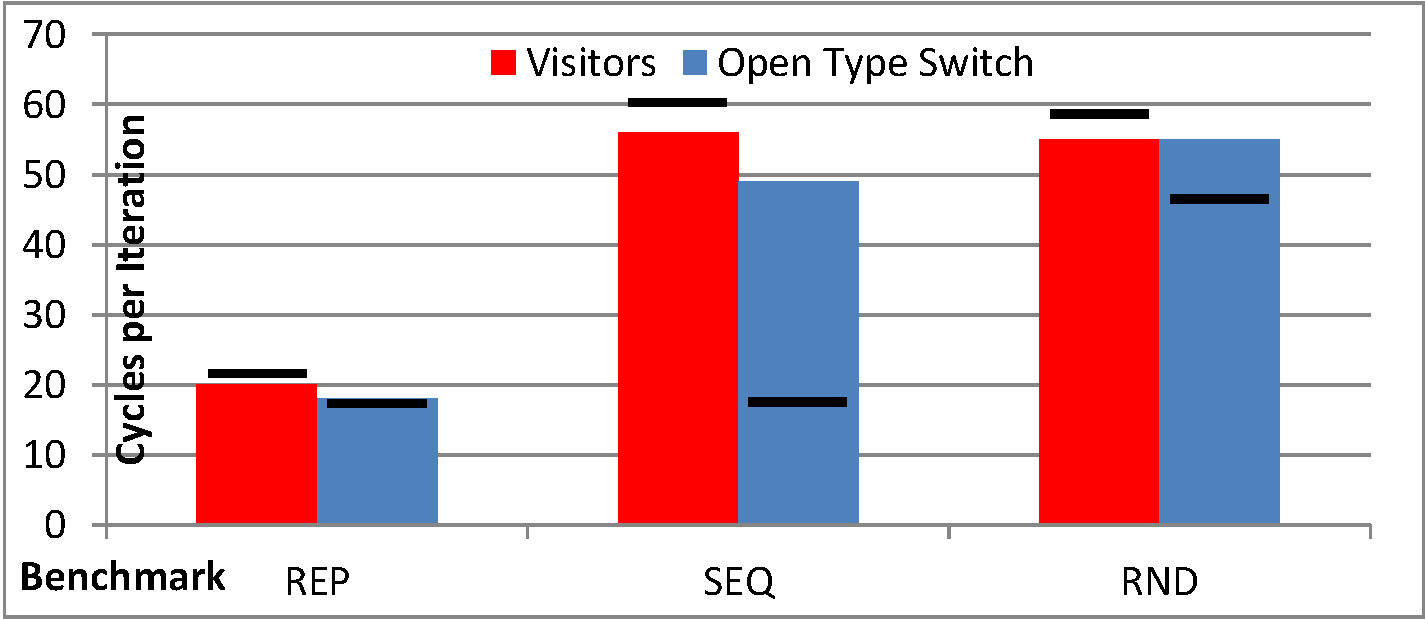
\includegraphics[width=0.47\textwidth]{VisitorsCompare.pdf}
  \caption{Absolute timings for different benchmarks}
  \label{fig:VisitorsComparison}
\end{figure}

To understand better the relative numbers of Figure~\ref{relperf}, we present 
in Figure~\ref{fig:VisitorsComparison} few absolute timings taken by visitors 
and open type switch to execute an iteration of a given benchmark. These absolute timings 
correspond to the relative numbers from column Open/G++/Win of Figure~\ref{relperf}.
The actual bars show the timings without forwarding, while the black lines 
indicate where the corresponding bar would be in the presence of forwarding. It 
is easy to see that visitors generally become slower in the presence of 
forwarding due to extra call, while type switch becomes faster due to smaller 
jump table. As discussed, both timings are much smaller for repetitive benchmark 
due to hardware cache.

Figure~\ref{relperf} provides a broader overview of how both techniques compare 
under different compiler/platform configurations. The values are given as 
percentages of performance increase against the slower technique. 
%Numbers in regular font represent cases where type switching was  
%faster, while underlined numbers in bold indicate cases where visitors were faster.

We can see that type switching wins by a good margin when implemented with tag switch (\textsection\ref{sec:cotc}) as  
well as in the presence of at least one level of forwarding. Note that the 
numbers are relative, and thus the ratio depends on both the performance of 
virtual function calls and the performance of switch statements. Visual \Cpp{} was 
generating faster virtual function calls, while GCC was generating faster switch 
statements, which is why their relative performance seem to be much more 
favorable for us in the case of GCC.
Similarly, the code for x86-64 is only slower relatively: the actual time spent for 
both visitors and type switching was smaller than that for x86-32, but it was much 
smaller for visitors than type switching, which resulted in worse relative 
performance.

The code on the critical path of our type switch implementation benefits 
significantly from branch hinting as some branches are much more likely than 
others. We use the branch hinting directives in GCC to guide the compiler, but, 
unfortunately, Visual \Cpp{} does not provide any similar facilities. Instead, 
Microsoft suggests using \emph{Profile-Guided Optimizations} (PGO) to achieve 
the same, which is why we list the results for Visual \Cpp{} both with and without 
profile-guided optimizations.
%The results without profile-guided optimizations can be 
%found in the accompanying technical report~\cite[\textsection 10]{TR}.
%The results of optimizing code created with Visual \Cpp{} by using profile 
%guided optimizations as currently Visual \Cpp{} does not have means for branch 
%hinting, which are supported by G++ and proven to be very effective in few 
%cruicial places. Profile guided optimization in Visual \Cpp{} lets compiler find 
%out experimentally what we would have otherwise hinted, even though this 
%includes other optimizations as well.

From the table it may seem that Visual C++ is generating not as good code as GCC 
does, but remember that these numbers are relative, and thus the ratio depends on  
both the performance of virtual calls and the performance of switch statements. Visual 
C++ was generating faster virtual function calls, while GCC was generating 
faster switch statements, which is why their relative performance seem to be much 
more favorable for us in the case of GCC.

Similarly the code for x64 is only slower relatively: the actual time spent for 
both visitors and type switching was smaller than that for x86, but it was much 
smaller for visitors than type switching, which resulted in worse relative 
performance.

\subsection{Open vs. Closed Type Switch}
\label{sec:cmp}

With only a few exceptions for x64, we saw in the Figure~\ref{relperf} that the 
performance of the closed tag switch (the Tag column) dominates the performance of the open type
swith (the Open column). We believe that the difference, often significant, is the price one pays 
for the true openness of the vtable pointer memoization solution.

As we mentioned in \textsection\ref{sec:cotc}, the use of tags, even when allocated 
by a compiler, may require integration efforts to ensure that different DLLs have 
not reused the same tags. Randomization of tags, similar to a proposal of 
Garrigue~\cite{garrigue-98}, will not eliminate the problem and will surely 
replace jump tables in switches with decision trees. This will likely 
significantly degrade the numbers for the part of Figure~\ref{relperf} 
representing closed tag switch, since the tags in our experiments were all 
sequential and small. 

The reliance of a tag switch on static cast, as described in \textsection\ref{sec:vtblmem}, this has severe limitations in the 
presence of multiple inheritance, and thus is not as versatile as open type 
switch. Overcoming this problem will either require the use of 
\code{dynamic_cast} or techniques similar to vtable pointer memoization, which 
will likely degrade tag switch's performance numbers even further.

Note also that the approach used to implement open type switch can be used to 
implement both first-fit and best-fit semantics, while the tag switch is only suitable 
for best-fit semantics. Their complexity guarantees also differ: open type 
switch is constant on average, but slow on the first call with given subobject. 
Tag switch is logarithmic in the size of the class hierarchy 
(assuming a balanced hierarchy), including the first call. This last point can 
very well be seen in Figure~\ref{relperf}, where the performance of a closed solution
degrades significantly in the presence of forwarding, while the performance of an
open solution improves.

\subsection{Comparison with OCaml and Haskell}
\label{sec:ocaml}

We now compare our solution to the built-in pattern-matching facility of 
OCaml~\cite{OPM01} and Haskell~\cite{Haskell98Book}.  
In this test, we timed small OCaml and Haskell applications performing our sequential 
benchmark on an algebraic data type of 100 variants. Corresponding \Cpp{} 
applications were working with a flat class hierarchy of 100 derived classes. 
The difference between the C++ applications lies in the encoding (Open/Tag/Kind) 
and the syntax (Unified/Special) used. Kind 
encoding is the same as Tag encoding, but it does not require substitutability, 
and thus can be implemented with a direct switch on tags without a ReMatch loop. 
It is only supported through specialized syntax in our library as it differs 
from the Tag encoding only semantically.

%The optimized OCaml compiler \texttt{ocamlopt.opt} that we used to compile the code 
%can be based on different toolsets on some platforms, e.g. Visual \Cpp{} or GCC 
%on Windows. To make the comparison fair we had to make sure that the 
%same toolset was used to compile the \Cpp{} code. We ran the tests 
%on both of the machines described above using the following configurations: 

%\begin{itemize}
%\setlength{\itemsep}{0pt}
%\setlength{\parskip}{0pt}
%\item The tests on a Windows 7 laptop were all based on the \emph{Visual \Cpp{} toolset} 
%      and used \texttt{ocamlopt.opt} version 3.11.0.
%\item The tests on a Linux desktop were all based on the \emph{GCC toolset} and used 
%      \texttt{ocamlopt.opt} version 3.11.2
%\end{itemize}

%\noindent
We used the optimizing OCaml compiler \texttt{ocamlopt.opt} version 3.11.0 working 
under the Visual \Cpp{} toolset as well as the Glasgow Haskell Compiler version 
7.0.3 (with -O switch) working under the MinGW toolset. The \Cpp{} applications 
were compiled with Visual \Cpp{} as well and all the tests were  
performed on the Windows 7 laptop. Similar to comparison with visitors,
the timing results presented in Figure~\ref{fig:OCamlComparison} are averaged 
over 101 measurements and show the number of seconds it took to perform a 
1,000,000 decompositions within our sequential benchmark. We compare here time 
and not cycles, as that was the only common measurement in all three 
environments.

\begin{figure}[htbp]
  \centering
    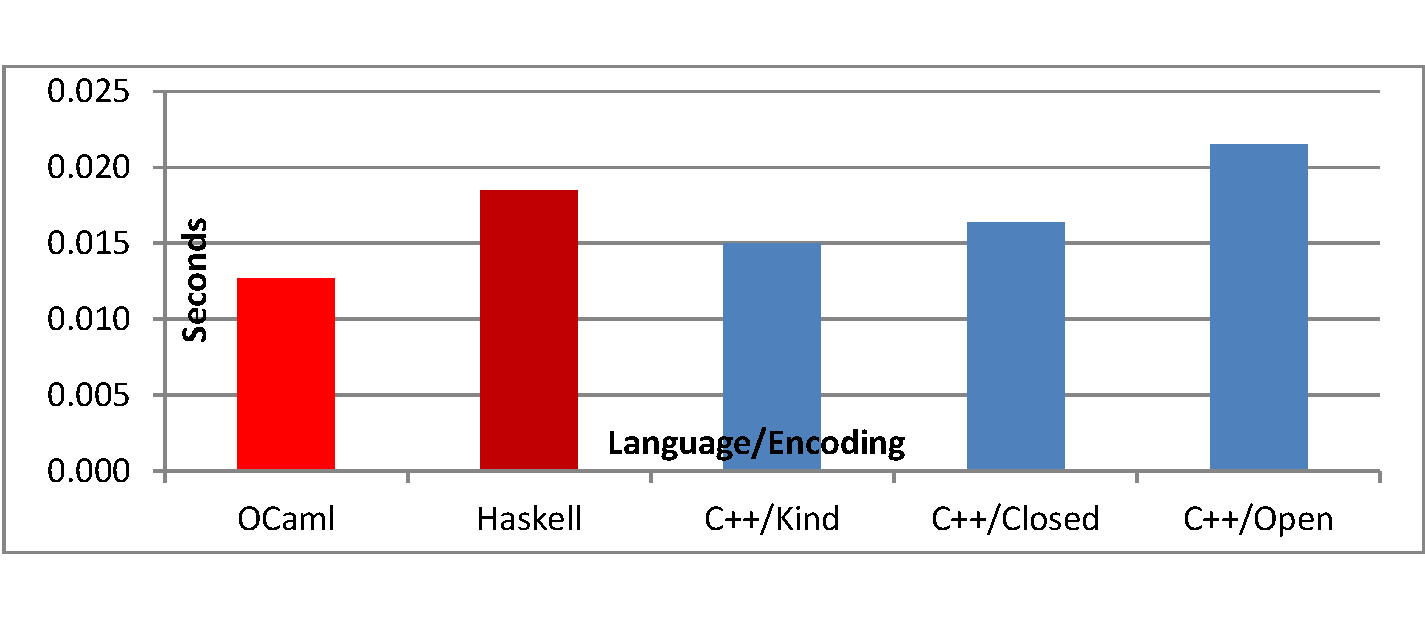
\includegraphics[width=0.47\textwidth]{OCamlComparison.pdf}
  \caption{Performance comparison with OCaml \& Haskell}
  \label{fig:OCamlComparison}
\end{figure}

We can see that the use of specialized syntax on a closed/sealed hierarchy can 
match the speed of, and even be four times faster than, the code generated by 
the native OCaml compiler. Once we go for an open solution, we become about 
30-50\% slower. 

\subsection{Dealing with real-world class hierarchies}
\label{sec:hierarchies}

For this experiment, we used a class hierarchy benchmark previously used in the 
literature to study efficiency of type inclusion testing and dispatching 
techniques~\cite{Vitek97,Krall97nearoptimal,PQEncoding,Ducournau08}.
We use the names of each benchmark from Vitek et al~\cite[Table 2]{Vitek97}, 
since the set of benchmarks we were working with was closest (though not exact) 
to that work.

While not all class hierarchies originated from \Cpp{}, for this experiment it 
was more important for us that the hierarchies were man-made. While converting 
the hierarchies into \Cpp{}, we had to prune inaccessible base classes (direct base  
class that is already an indirect base class) when used with repeated 
inheritance in order to satisfy semantic requirements of \Cpp{}. We maintained 
the same number of virtual functions present in each class as well as the number 
of data members; the benchmarks, however, did not preserve the exact types of those.
The data in Figure~\ref{fig:benchmarks} shows various parameters of the class 
hierarchies in each benchmark, after their adoption to \Cpp{}. 

\begin{figure}[htbp]
\footnotesize
\begin{tabular}{@{ }l@{ }||@{ }l@{ }|@{ }r@{ }|@{ }r@{ }|@{ }r@{ }|@{ }r@{ }|@{ }r@{ }|@{ }r@{ }|@{ }l@{ }|@{ }r@{ }|@{ }r@{ }|@{ }r@{ }}
\hline % --------------------------------------------------------------------------------------------------
\multicolumn{1}{@{}c@{}||}{\multirow{2}{*}{\tiny{\textsc{Library}}}} & 
\multicolumn{1}{@{ }c@{ }|}{\multirow{2}{*}{\tiny{\textsc{Language}}}} & 
\multicolumn{1}{@{ }c@{ }|}{\multirow{2}{*}{\tiny{\textsc{Classes}}}} &
\multicolumn{1}{@{ }c@{ }|}{\multirow{2}{*}{\tiny{\textsc{Paths}}}} & 
\multicolumn{1}{@{ }c@{ }|}{\multirow{2}{*}{\tiny{\textsc{Height}}}} & 
\multicolumn{1}{@{ }c@{ }|}{\multirow{2}{*}{\tiny{\textsc{Roots}}}} & 
\multicolumn{1}{@{ }c@{ }|}{\multirow{2}{*}{\tiny{\textsc{Leafs}}}} & 
\multicolumn{1}{@{ }c@{ }|}{\multirow{2}{*}{\tiny{\textsc{Both}}}} & 
\multicolumn{2}{@{}c@{}|}{\tiny{\textsc{Parents}}} & 
\multicolumn{2}{@{}c@{}}{\tiny{\textsc{Children}}} \\ \cline{9-12}
     &                             &      &       &    &     &      &     & \multicolumn{1}{@{}c@{}|}{\tiny{\textsc{avg}}} & \multicolumn{1}{@{}c@{}|}{\tiny{\textsc{max}}} & \multicolumn{1}{@{}c@{}|}{\tiny{\textsc{avg}}} & \multicolumn{1}{@{}c@{}}{\tiny{\textsc{max}}} \\
\hline % --------------------------------------------------------------------------------------------------
 DG2 & \tiny{\textsc{Smalltalk}}   &  534 &   534 & 11 &   2 &  381 &   1 & 1    &  1 & 3.48 &  59 \\ % digitalk2         
 DG3 & \tiny{\textsc{Smalltalk}}   & 1356 &  1356 & 13 &   2 &  923 &   1 & 1    &  1 & 3.13 & 142 \\ % digitalk3         
 ET+ & \tiny{\textsc{\Cpp{}}}      &  370 &   370 &  8 &  87 &  289 &  79 & 1    &  1 & 3.49 &  51 \\ % et++              
 GEO & \tiny{\textsc{Eiffel}}      & 1318 & 13798 & 14 &   1 &  732 &   0 & 1.89 & 16 & 4.75 & 323 \\ % geode             
 JAV & \tiny{\textsc{Java}}        &  604 &   792 & 10 &   1 &  445 &   0 & 1.08 &  3 & 4.64 & 210 \\ % java              
 LOV & \tiny{\textsc{Eiffel}}      &  436 &  1846 & 10 &   1 &  218 &   0 & 1.72 & 10 & 3.55 &  78 \\ % lov-object-editor 
 NXT & \tiny{\textsc{Objective-C}} &  310 &   310 &  7 &   2 &  246 &   1 & 1    &  1 & 4.81 & 142 \\ % nextstep          
 SLF & \tiny{\textsc{Self}}        & 1801 & 36420 & 17 &  51 & 1134 &   0 & 1.05 &  9 & 2.76 & 232 \\ % self              
 UNI & \tiny{\textsc{\Cpp{}}}      &  613 &   633 &  9 & 147 &  481 & 117 & 1.02 &  2 & 3.61 &  39 \\ % unidraw           
%    &                             &   51 &    51 &  7 &   1 &   29 &   0 & 1.00 &  1 & 2.27 &   5 \\ % v1-collection     
%    &                             &   18 &    18 &  5 &   1 &   11 &   0 & 1.00 &  1 & 2.43 &   5 \\ % v1-magnitude      
%    &                             &  383 &   383 &  9 &   1 &  244 &   0 & 1.00 &  1 & 2.75 &  86 \\ % v1-object-nometa  
%    &                             &    9 &     9 &  5 &   1 &    4 &   0 & 1.00 &  1 & 1.60 &   2 \\ % v1-set            
%    &                             &   16 &    16 &  7 &   1 &    7 &   0 & 1.00 &  1 & 1.67 &   2 \\ % v1-stream         
%    &                             &   53 &    53 &  8 &   1 &   31 &   0 & 1.00 &  1 & 2.36 &   7 \\ % v1-visualcomponent
 VA2$_a$& \tiny{\textsc{Smalltalk}}& 3241 &  3241 & 14 &   1 & 2582 &   0 & 1    &  1 & 4.92 & 249 \\ % visualage2.all    
 VA2$_k$& \tiny{\textsc{Smalltalk}}& 2320 &  2320 & 13 &   1 & 1868 &   0 & 1    &  1 & 5.13 & 240 \\ % visualage2.kern   
 VW1 & \tiny{\textsc{Smalltalk}}   &  387 &   387 &  9 &   1 &  246 &   0 & 1    &  1 & 2.74 &  87 \\ % visualworks1      
 VW2 & \tiny{\textsc{Smalltalk}}   & 1956 &  1956 & 15 &   1 & 1332 &   0 & 1    &  1 & 3.13 & 181 \\ % visualworks2      
%    &                             &    6 &     9 &  4 &   2 &    1 &   0 & 1.50 &  2 & 1.20 &   2 \\ % vtbl              
\hline % --------------------------------------------------------------------------------------------------
\multicolumn{2}{r|}{\tiny{\textsc{Overalls}}} &15246 & 63963 & 17 & 298 &10877 & 199 & 1.11 & 16 & 3.89 & 323 \\ % Overalls
\hline % --------------------------------------------------------------------------------------------------
\end{tabular}
\caption{Benchmark class hierarchies}
\label{fig:benchmarks}
\end{figure}

The number of paths represents the number of distinct inheritance paths from the 
classes in the hierarchy to the roots of the hierarchy. This number reflects the number of possible subobjects in the 
hierarchy. The roots listed in the table are classes with no base classes. We 
will subsequently use the term \emph{non-leaf} to refer to the possible root of 
a subhierarchy. Leafs are classes with no children, while \emph{both} refers to 
utility classes that are both roots and leafs and thus neither have base nor 
derived classes. The average for the number of parents and the number of 
children were computed only among the classes having at least one parent or at 
least one child correspondingly.

With few useful exceptions, it generally makes sense to apply type switch only 
to non-leaf nodes of the class hierarchy. 71\% of the classes in the entire 
benchmarks suite were leaf classes. Out of the 4369 non-leaf classes, 36\% were 
spawning a subhierarchy of only 2 classes (including the root), 15\% -- a 
subhierarchy of 3 classes, 10\% of 4, 7\% of 5 and so forth. 
Turning this into a cumulative distribution, $a\%$ of subhierarchies had more 
than $b$ classes in them:

%\noindent
\begin{tabular}
{l||@{ }c@{ }|@{ }c@{ }|@{ }c@{ }|@{ }c@{ }|@{ }c@{ }|@{ }c@{ }|@{ }c@{ }|@{ }c@{ }|@{ }c@{ }}
%{l||c|c|c|c|c|c|c|c|c}
$a$ & 1\% & 3\% & 5\% & 10\% & 20\% & 25\% & 50\% & 64\% & 100\% \\
\hline % --------------------------------------------------------------------------------------------------
$b$ & 700 & 110 & 50  & 20   & 10   & 7    & 3    & 2    & 1
\end{tabular}

%1\% of subhierarchies had more than 700 classes in them, 3\% of subhierarchies 
%had more than 110 classes, 5\% of subhierarchies had more than 50 classes, 10\% 
%of subhierarchies had more than 20 classes, 20\% of subhierarchies had more than 
%10 classes, 25\% of hierarchies had more than 7 classes, only 50\% of 
%hierarchies had more than 3 classes and 64\% -- more than 2.

\noindent
These numbers reflect the percentage of use cases one may expect in the real 
word that have a given number of case clauses in them.

For each non-leaf class $A$ we created a function performing a type switch on 
every possible derived class $D_i$ of it as well as itself. The function was 
then executed with every possible subobject $D_i\leftY\sigma_j\rightY A$ it can  
possibly be applied to, given the static type $A$ of the subject. It was 
executed multiple but the same number of times on each subobject to ensure 
uniformity on one side (since we do not have the data about the actual 
probabilities of each subobject in the benchmark hierarchies) as well as let the 
type switch infer the optimal parameters $k$ and $l$ of its cache indexing 
function $H_{kl}^V$. We then plotted a point in chart of Figure~\ref{fig:prob} 
relating 2 characteristics of each of the 4396 type switches tested: the optimal 
computed probability of conflict $p$ achieved by the type switch and the number 
of subobjects $n$ that came through that type switch. The actual frequencies of 
collisions were within one tenth of a percentage point of the computed 
probabilities, which is why we did not use them in the chart. To account for the 
fact that multiple experiments could have resulted in the same pair $(n,p)$, we 
use a shadow of each point to reflect somewhat the number of experiments 
yielding it.

\begin{figure}[htbp]
  \centering
    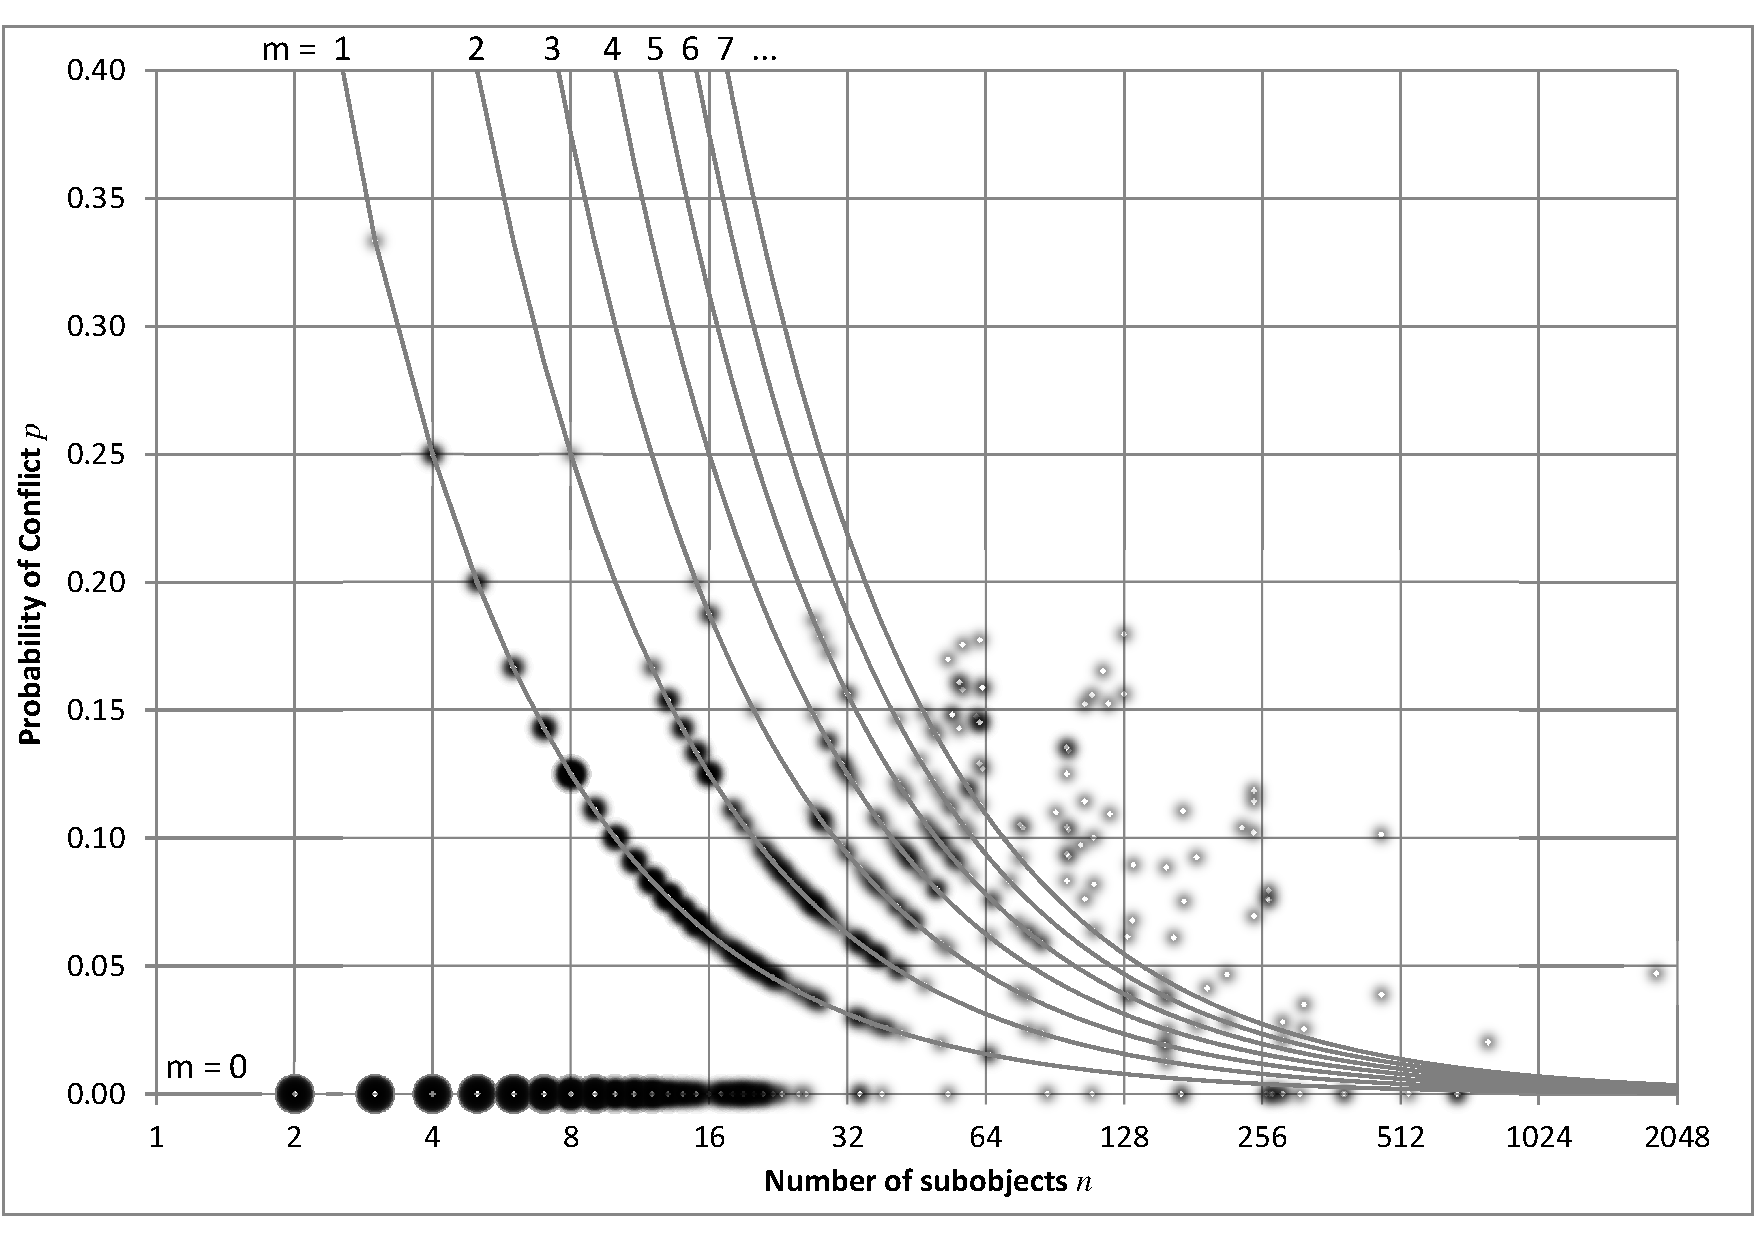
\includegraphics[width=0.49\textwidth]{ClassHierarchies.pdf}
  \caption{Probability of conflict in real hierarchies}
  \label{fig:prob}
\end{figure}

The curves on which the results of experiments line up correspond to the fact 
that under uniform distribution of $n$ subobjects, only a finite number of 
different values representing the probability of conflict $p$ is possible. In 
particular, all such values $p=\frac{m}{n}$, where $0 \le m < n$. The number $m$ 
reflects the number of subobjects an optimal cache indexing function $H_{kl}^V$ 
could not allocate their own entry for and we showed in \textsection\ref{sec:moc} 
that the probability of conflict under uniform distribution of $n$ subobjects 
depends only on $m$. The curves thus correspond to graphs of functions 
$y=\frac{m}{x}$ for different values of $m$. The points on the same curve (which 
becomes a line on a log-log plot) all share the same number $m$ of ``extra'' 
vtbl-pointers that optimal cache indexing function could not allocate individual 
entries for.

While it is hard to see from the chart, 87.5\% of all the points on the chart 
lay on the X-axis, which means that the optimal hash function for the 
corresponding type switches had no conflicts at all ($m=0$). In other words, only in 12.5\% 
of cases the optimal $H_{kl}^V$ for the set of vtbl-pointers $V$ coming through 
a given type switch had non-zero probability of conflict. Experiments laying on 
the first curve amount to 5.58\% of subhierarchies and represent the cases in 
which optimal $H_{kl}^V$ had only one ``extra'' vtbl-pointer ($m=1$). 2.63\% of 
experiments had $H_{kl}^V$ with 2 conflicts, 0.87\% with 3 and so forth as shown 
in Figure~\ref{fig:size}($K+1$).

\begin{figure}[htbp]
\small
\begin{tabular}
{@{}c@{}||@{}c@{ }|@{}c@{ }|@{}c@{ }|@{}c@{ }|@{}c@{ }|@{}c@{ }|@{}c@{ }|@{}c@{ }}
\hline % -------------------------------------------------------------------------
  $m$ &       0 &       1 &      2 &      3 &      4 &        5 &      6 & \textgreater 6 \\
\hline % -------------------------------------------------------------------------
$K+1$ & 87.50\% &  5.58\% & 2.63\% & 0.87\% & 0.69\% & 0.69\% & 0.30\% & 1.76\% \\
\hline % -------------------------------------------------------------------------
  $K$ & 72.55\% & 12.27\% & 4.87\% & 2.61\% & 1.42\% & 0.94\% & 0.80\% & 4.55\% 
\end{tabular}
\caption{Percentage of type switches with given number of conflicts ($m$) under different size constraints}
\label{fig:size}
\end{figure}

In cases when the user is willing to trade performance for better space 
efficiency she may restrict $k$ to $[K,K]$ instead of $[K,K+1]$ as discussed in 
\textsection\ref{sec:moc}. We redid all the 4396 experiments under this 
restriction and obtained a similar histogram shown in Figure~\ref{fig:size}($K$).
The average probability of conflict over the entire set increased from 0.011 to 
0.049, while the maximum probability of conflict increased from 0.333 to 0.375. 
The average load factor of the cache expectedly increased from 75.45\% to 82.47\%. 

It is important to understand that the high ratio of cases in which the hash 
function could deliver perfect indexing does not indicate that the hash function 
we used is better than other hash functions. It does indicate instead that the 
values representing vtbl-pointers in a given application are not random at all and 
are particularly suitable for such a hash function.

\subsection{Refactoring an existing visitors based application}
\label{sec:qualcmp}

For this experiment, we reimplemented a visitor based \Cpp{} pretty printer for 
Pivot\cite{Pivot09} using \emph{Mach7}. The Pivot's class hierarchy 
consists of 154 node kinds representing various entities in the \Cpp{} program. The 
original code had 8 visitor classes each handling 5, 7, 8, 10, 15, 17, 30 and 63 
cases, which we turned into 8 match statements with corresponding numbers of 
case clauses. Most of the rewrite was performed by sed-like replaces that 
converted visit methods into respective case-clauses. In several cases we had to 
manually reorder case-clauses to avoid redundancy as visit-methods for base classes 
were typically coming before the same for derived, while for type switching we 
needed them to come after due to first-fit semantics. Redundancy checking 
support provided by \emph{Mach7} and discussed in \textsection\ref{sec:redun} was invaluable in finding all such cases.

During this refactoring we have made several simplifications that became obvious 
in pattern-matching code, but were not in visitors code because of control 
inversion. Simplifications that were applicable to visitors code were eventually 
integrated into visitors code as well to make sure we do not compare 
algorithmically different code. In any case we were making sure that both 
approaches regardless of simplifications were producing byte-to-byte the same 
output as the original pretty printer we started from.

The size of executable for pattern-matching approach was smaller than that for 
visitors. So was also the source code. We extracted from both sources the 
functionality that was common to them and placed it in a separate translation 
unit to make sure it does not participate in the comparison. We kept all the 
comments however that were eqaully applicable to code in either approach.

Both pretty printers were executed on a set of header files from the \Cpp{} 
standard library and the produced output of both program was byte-to-byte the same. 
We timed execution of the pretty printing phase (not including loading and termination 
of the application or parsing of the source file) and observed that on small 
files (e.g. those from C run-time library and few small \Cpp{} files) 
visitors-based implementation was faster because the total number of nodes in 
AST and thus calls did not justify our set-up calls. In particular, 
visitor-based implementation of the pretty printer was faster on files of 44--588  
lines of code, with average 136 lines per those inputs, where visitors win. On 
these input files, visitors are faster by 1.17\%--21.42\% with an average speed-up of 
8.75\%. Open type switch based implementation of the pretty printer was faster on 
files of 144--9851 lines of code, with average 3497 lines per those input files, 
where open type switch wins. On these inputs, open type switch is faster by 0.18\% -- 32.99\% 
with an average speed-up of 5.53\%.

Figure~\ref{fig:mem} shows memory usage as well as cache hits and misses for 
the run of our pretty printer on \code{<queue>} standard library 
header, which had the largest LOC count after preprocessing in our test set.

\begin{figure}[htbp]
  \centering
    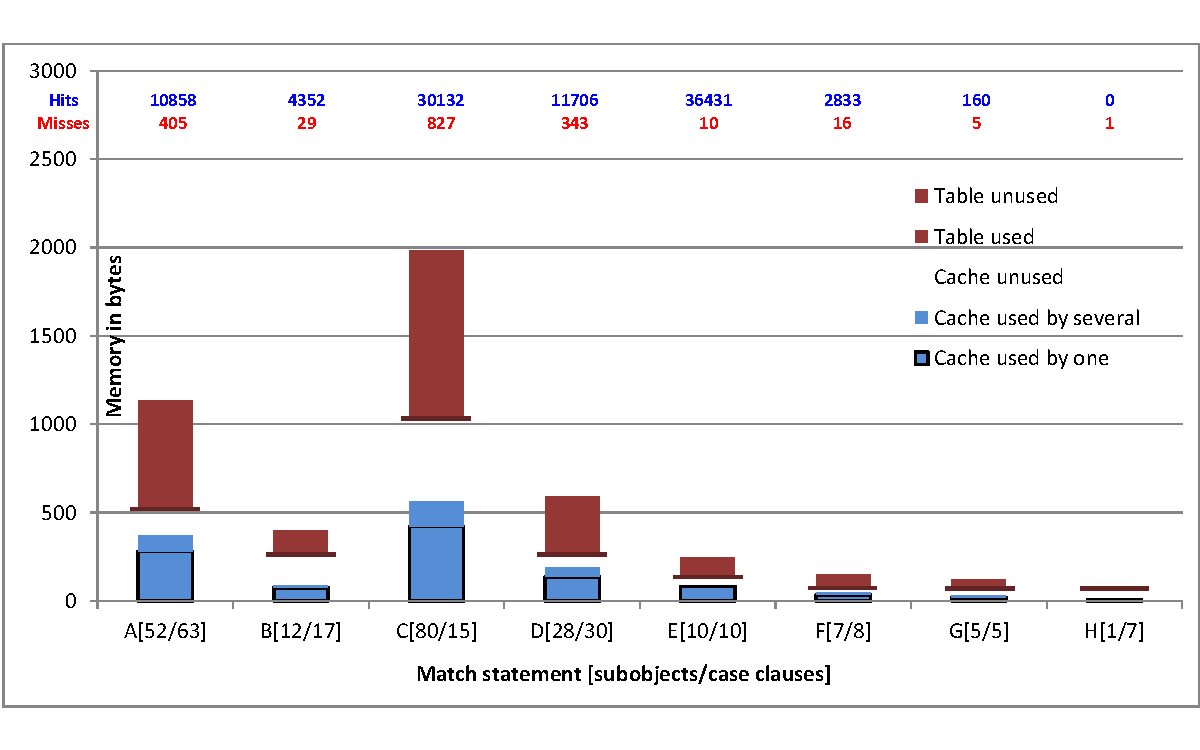
\includegraphics[width=0.49\textwidth]{Memory.pdf}
  \caption{Memory usage in real application}
  \label{fig:mem}
\end{figure}

The bars represent the total size of memory in bytes each of the 8 match 
statements (marked A-H) used. Information $[n/c]$ next to the letter indicates the 
actual number of different subobjects (i.e. vtbl-pointers) $n$ that came through 
that match statement, and the number of case clauses $c$ the match statement had 
(the library uses $c$ as an estimate of $n$). $n$ is also the number of cases the 
corresponding match statement had to be executed sequentially (instead of a 
direct jump).

The lower part of each bar (with respect to dividing line) corresponds to the memory used by cache, while the 
upper part -- to the memory used by the hash table. The ratio of the darker
section of each part to the entire part indicates the load factors 
of cache and hash-table respectively. The black box additionally indicates the 
proportion of cache entries that are allocated for only one vtbl-pointer and 
thus never result in a cache miss. %The non-transparent part without black box 
%represents the percentage of vtbl-pointers that have to share their cache entry 
%with at least one other vtbl-pointer and thus may result in collisions during 
%access.

The actual number of hits and misses for each of the match statements is 
indicated on top of the corresponding column. The sum of them is the total 
number of calls made. %Hits indicate situation when we found entry in cache and 
%didn't have to make roundtrip to the hash-table to get it. Misses indicate the 
%number of cases during actual run we had to pick the entry from the hash table 
%and update the cache with it. 
The number of misses is always larger than or equal to $n$ since we need to 
execute the switch sequentially on each of them once in order to memoize the 
outcome.

The library always preallocates memory for at least 8 subobjects to avoid 
unnecessary recomputations of optimal parameters $k$ and $l$ -- this is the case 
with the last 3 match statements. In all other cases it allocates the 
memory proportional to $2^{K+1}$ where $2^{K-1} < \max(n,c) \le 2^{K}$. We make 
$c$ a parameter, because in a library setting $n$ is not known up front and 
estimating it with $c$ allows us to avoid unnecessary recomputations of $l$ and 
$k$ even further. 

The table does not have to be hash table and can be implemented with 
any other container i.e. sorted vector, map etc. that let us find quickly by a given 
vtbl-pointer the data associated with it. In fact we provide a slightly less 
efficient caching container that avoids the table altogether, thus significantly 
reducing the memory requirements instead.

%During this refactoring we have made several simplifications that became obvious 
%in pattern-matching code, but were not in visitors code because of control 
%inversion. Simplifications that were applicable to visitors code were eventually 
%integrated into visitors code as well to make sure we do not compare 
%algorithmically different code. In any case we were making sure that both 
%approaches regardless of simplifications were producing byte-to-byte the same 
%output as the original pretty printer we started from.

%The size of executable for pattern-matching approach was smaller than that for 
%visitors. So was also the source code. We extracted from both sources the 
%functionality that was common to them and placed it in a separate translation 
%unit to make sure it does not participate in the comparison. We kept all the 
%comments however that were eqaully applicable to code in either approach.
%
Note that the visitors involved in the pretty printer above did not use 
forwarding: since all the \Cpp{} constructs were handled by the printer, every 
visit-method was overriden from those statically possible based on the static 
type of the argument.

Listing parameter for a case clause always causes access to member. Best hope is 
that compiler will eliminate it if it is not needed. At the moment we do not 
have means to detect empty macro arguments or \_.

In general from our rewriting experience we will not recommend rewriting 
existing visitor code with pattern matching for the simple reason that pattern 
matching code will likely follow the structure already set by the visitors. 
Pattern matching was most effective when writing new code, where we could design 
the structure of the code having the pattern-matching facility in our toolbox.

\subsection{Limitations}
\label{sec:lim}

Currently the definition of each class used in a case clause must be visible to 
the compiler because \code{dynamic_cast} operator used in the type switch does 
not allow incomplete types as a target type. For particularly large type 
switches (e.g. \textgreater 1000 case clauses) this may easily reach some 
compiler limitations. Both GCC and Visual \Cpp{}, for example, could not generate 
object files for such translation units simply because the sheer size of v-tables 
and other compiler data in it were exceeding the limits. The problem is not 
specific to our technique though and allowing \code{dynamic_cast} on classes 
that were declared but not defined yet would solve the problem.

While it might be reasonable to expect from linkers to layout v-tables close 
to each other -- the property that makes our hashing function efficient -- they 
are not required to do so. We believe, nevertheless, that should our approach 
become popular through the library implementation, its compiler implementation 
will encourage compiler vendors to enforce the property in order to keep the 
type switching fast.

\section{Related Work} %%%%%%%%%%%%%%%%%%%%%%%%%%%%%%%%%%%%%%%%%%%%%%%%%%%%%%%%%
\label{sec:rw}

Language support for pattern matching was first introduced for string manipulation 
in COMIT\cite{COMIT58}, which subsequently inspired similar primitives in 
SNOBOL\cite{SNOBOL64}. SNOBOL4 had string patterns as first-class data types 
providing operations of concatenation and alternation\cite{SNOBOL71}.
The first reference to a modern pattern-matching constructs seen in functional 
languages is usually attributed to Burstall's work on structural 
induction\cite{Burstall69provingproperties}. Pattern matching was further 
developed by the functional programming community, most notably 
Hope\cite{BMS80}, Miranda\cite{Miranda85}, ML\cite{ML90} and 
Haskell\cite{Haskell98Book}. In the context of object-oriented programming, 
pattern matching has been first explored in Pizza\cite{Odersky97pizzainto} and 
Scala\cite{Scala2nd,EmirThesis}. The idea of first class patterns dates back to 
at least Tullsen's proposal to add them to Haskell~\cite{Tullsen00}, calculus of 
such patterns has been studied in details by Jay~\cite{Jay09,PatCalc09}.

There are two main approaches to compiling pattern-matching code: the first is 
based on \emph{backtracking automata} and was introduced by Augustsson\cite{Augustsson85}, 
the second is based on \emph{decision trees} and was first described by 
Cardelli\cite{Cardelli84}, though he attributes the technique to Dave MacQueen 
and Gilles Kahn in their implementation of the Hope compiler \cite{BMS80}.
Backtracking approach usually generates smaller code~\cite{OPM01}, while decision tree 
approach produces faster code by ensuring that each primitive test is only 
performed once~\cite{Maranget08}. With respect to matching a single expression our library 
approach follows the naive backtracking approach, however our match statement is 
based on a highly efficient type switching technique we developed\cite{TypeSwitch} 
that outperforms similar solutions based on decision trees or visitor design pattern.

Memoization device we proposed is not specifically concerned with compiling 
pattern matching and can be used independently. In particular it can be combined 
with either backtracking or decision tree approaches to avoid subsequent 
decisions on datum that has already been seen.

\emph{MatchO} was one of the first attempts to implement pattern matching without 
extending the host language~\cite{Visser06matchingobjects}. While the library 
was essentially providing first class patterns into Java, the amount of 
syntactic and run-time overhead was overwhelming. The author offers to provide 
customized syntax to patterns by invoking an inline parser, while to improve 
performance the author looks into combining visitors and visitor combinators 
with pattern matching. %This resembles our use of an efficient type switch to 
%uncover the dynamic type combined with slower but more flexible pattern 
%matching.

\emph{Functional C\#} was a similar approach to bringing pattern matching into 
C\# as a library\cite{FuncCSharp}. The approach uses lambda functions and 
chaining of method calls to create a structure that is then evaluated at 
run-time for the first successful match. The approach supports a form of 
active patterns, simple n+k patterns, list and tuple patterns as well as type 
patterns (without structural decomposition). Unfortunately, the solution scales 
very poorly for match statements with more than two case clauses as it is 
essentially based on sequential type tests. Besides, the approach is ill suited 
for tests involving nesting of patterns.

Both \emph{MatchO} and \emph{Functional C\#} were object-oriented solutions. In 
functional community, Rhiger explored a similar idea of introducing pattern 
matching into Haskell as a library~\cite{Rhiger09}. He uses functions to encode 
patterns and pattern combinators, which allows him to detect pattern 
misapplication errors at compile time through the Haskell type system. 
Unfortunately, the purity of a functional language prevents him from expressing 
variable patterns (more specifically, the bindings they introduce) in a library 
setting simply, which then affects the overal ellegance of the solution. In 
particular, it seems to be impossible in his approach to express equivalence 
patterns or even equivalence combinator as the value of the bound variable is 
not available in the left-hand side of the matching expression, only in the 
right-hand side. The library is sufficiently expressive though to express basic 
patterns (value, wildcard, predicate, etc.), boolean pattern combinators and set 
patterns. The author reports that his solution requires 2-4 times more 
reductions than Haskell's built-in pattern matching. He attributes the overhead 
to currying and continuations passing and hypothsizes that it should be completly 
eliminated by standard partial evaluation techniques.

\emph{Grace} is another programming language that provides a library solution to 
pattern matching through objects~\cite{Grace2012}. The language is aimed at 
teaching various programming paradigms and has an interesting peculiarity: it 
does not have pre-defined control structures, which instead are expressed 
directly in the language with the help of partial functions and lambda 
expressions. The \codeocaml{match}-statement, for example, takes form of a 
clausal definition \codeocaml{match(e)case(c1)...case(cn)}, specialized for 
large values of $n$. 
 
this with clausal function  
definitions i.e. if(c)then(b1)else(b2) with blocks (lambda expressions) passed 
as second and third parameter. They provide match(e)case(c1)...case(cn) for some 
large number n (cleanly) and have a workaround that hardcodes in the compiler 
support for arbitrary number of cases. Patterns are objects in Grace that are 
composed and applied at run-time. The compiler has some syntactic sugar to 
denote some most commone ones, but otherwise user-defined patterns have to be 
created explicitly. Grace has structural subtyping, not a nominative one, so 
their case analysis is never hierarchical like in our case. The approach does 
not seem to provide for optimizations.  I spoke with one of the authors, who 
presented the slides and he said that performance was indeed not a concern for 
them and only the expressiveness of the language and ease of its teaching to 
students was. The paper is not directly related to type switch, however it is 
related to the second pattern-matching paper. It also mentions some interesting 
works I haven't seen before that we will have to discuss in the second paper. 
%xxxxxxxxxxxxxxxxxxxxxxxxxxxxxxxxxxxxxxxxxxxxxxxxxxxxxxxxxxxxxxxxxxxxxxx

\emph{Lookup caches} have been long used to reduce the overhead of 
dynamically-bound message passing in Smalltalk~\cite{UngarPatterson83}. 
\emph{Inline caching} improves on that by noting that the type of the receiver at a given 
call site rarely varies so that the call instruction can be speculatively 
modified to jump directly to a previously looked up method~\cite{Deutsch84}. 
In this case, the method must ensure that the type of the receiver has 
not changed and redirect the call to generic lookup otherwise. The effects of 
inline caching on modern architectures can be seen through hardware call target 
prediction, which in our case is exemplified by repetitive benchmark: both 
virtual function calls and the underlying jump-table implementation of the 
\code{Match}-statement are about twice as fast as usual.

\emph{Polymorphic Inline Caches}~\cite{Holzle:Chambers:Ungar:91} generalize the 
idea of inline caches further by building a decision tree in the method prologue 
that caches all lookup results. The main difference of this approach from our 
work is that it requires code generation at run time, while we do not require
re-compilation, re-linking or any computations in case of dynamic linking.
The reason for this is the difference in the initial setting: they map an
arbitrary number of receiver types to an arbitrary number of implementations, while 
we map an arbitrary number of receivers to a fixed number of jump 
targets. This lets us generate code at compile time that incorporates both the 
initial and memoized execution.

\emph{Extensible Visitors with Default Cases}~\cite[\textsection 
4.2]{Zenger:2001} attempt to solve the extensibility problem of visitors; 
however, the solution, after 
remapping it onto C++, has problems of its own. The visitation interface 
hierarchy can easily be grown linearly (adding new cases for the new classes in 
the original hierarchy each time), but independent extensions by different  
authorities require developer's intervention to unify them all, before they can 
be used together. This may not be feasible in environments that use dynamic 
linking. To avoid writing even more boilerplate code in new visitors, the 
solution would require usage of virtual inheritance, which typically has 
an overhead of extra memory dereferencing. On top of the double dispatch already 
present in the visitor pattern, the solution will incur two additional virtual 
calls and a dynamic cast for each level of visitor extension. Additional double 
dispatch is incurred by forwarding of default handling from a base visitor to a 
derived one, while the dynamic cast is required for safety and can be replaced 
with a static cast when the visitation interface is guaranteed to be grown linearly 
(extended by one authority only). Yet another virtual call is required to be 
able to forward computations to subcomponents on tree-like structures to the 
most derived visitor. This last function lets one avoid the necessity of using 
the heap to allocate a temporary visitor through the \emph{Factory Design 
Pattern}~\cite{DesignPatterns1993} used in the \emph{Extensible Visitor} solution 
originally proposed by Krishnamurti, Felleisen and Friedman~\cite{Krishnamurthi98}.

In order to address the expression problem in Haskell, L\"{o}h and Hinze proposed to 
extend its type system with open data types and open functions~\cite{LohHinze2006}.
Their solution allows the user to mark top-level data types and functions as 
open and then provide concrete variants and overloads anywhere in the program. 
Open data types are extensible but not hierarchical, which largely avoids the 
problems discussed here. The semantics of open extension is given by 
transformation into a single module, where all the definitions are seen in one 
place. This is a significant limitation of their approach that prevents it from 
being truly open, since it essentially assumes a whole-program view, which 
excludes any extension via DLLs. As is the case with many other implementations 
of open extensions, the authors rely on the closed world for efficient 
implementation: in their implementation, \emph{``data types can only be entirely 
abstract (not allowing pattern matching) or concrete with all constructors with 
the reason being that pattern matching can be compiled more efficiently if the 
layout of the data type is known completely''}. The authors also believe that 
\emph{there are no theoretical difficulties in lifting this restriction, but it 
might imply a small performance loss if closed functions pattern match on open 
data types}. Our work addresses exactly this problem, showing that it is not 
only theoretically possible but also practically efficient and in application to 
a broader problem.

Andrew Kennedy et al~\cite{GADTOOP05} considered encoding of generalized 
algebraic data types~\cite{SPJ06} using visitor design patterns in C\#.  That 
translation made essential use of generic methods, the equivalent of ``virtual 
function template'' (as they would be called if such functionalities existed in 
C++) to handle some of the open set aspects of GADTs.

Polymorphic variants in OCaml~\cite{garrigue-98} allow the addition of new variants 
later. They are simpler, however, than object-oriented extensions, as they do not 
form subtyping between variants themselves, but only between combinations of them. 
This makes an important distinction between \emph{extensible sum types} like 
polymorphic variants and \emph{extensible hierarchical sum types} like classes.
An important property of extensible sum types is that each value of the 
underlying algebraic data type belongs to exactly one disjoint subset, tagged with 
a constructor. The \emph{nominative subtyping} of object-oriented languages does 
not usually have this disjointness making classes effectively have multiple 
types. In particular, the case of disjoint constructors can be seen as a 
degenerated case of a flat class hierarchy among the multitude of possible class 
hierarchies.

Tom is a pattern-matching compiler that can be used together with Java, C or 
Eiffel to bring a common pattern matching and term rewriting syntax into the 
languages\cite{Moreau:2003}. It works as a preprocessor that transforms 
syntactic extensions into imperative code in the target language. Tom is quite 
transparent as to the concrete target language used and can potentially be 
extended to other target languages besides the three supported now. In 
particular, it never uses any semantic information of the target language during 
the compilation process and it does not inspect nor modify the source language 
part (their preprocessor is only aware of parenthesis and block delimiters of 
the source language). Tom has a sublanguage called Gom that can be used to 
define algebraic data types in a uniform mannaer, which their preprocessor then 
transforms into conrete definitions in the target language. Alternatively, the 
user can provide mappings to his own data structures that the preprocessor will 
use to generate the code.

In comparison to our approach Tom has much bigger goals. The combination of 
pattern matching, term rewriting and strategies turns Tom into a 
tree-transformation language similar to Stratego/XT, XDuce and others. 
The main accent is made on expressivity and the speed of development, which 
makes one often wonder about the run-time complexity of the generated code.
Tom's approach is also prone to general problems of any preprocessor based 
solution\cite[\textsection 4.3]{SELL}. For example, when several preprocessors 
have to be used together, each independent extension may not be able to 
understand the other's syntax, making it impossible to form a toolchain.
A library approach we follow avoids most of these problems by relying only on a 
standard C++ compiler. It also lets us employ the C++ semantics within 
patterns: e.g. our patterns work directly on underlying user-defined data 
structures, largely avoiding abstraction penalties. The tight integration with 
the language semantics also makes our patterns first-class citizens that can be 
composed and passed to other functions. The approach we take to type switching 
can also be used by Tom's preprocessor to implement type patterns efficiently -- 
similarly to other object-oriented languages, Tom's handling of them is based on 
highly inefficient \code{instanceof} operator and its equivalents in other 
languages.

Pattern matching in Scala~\cite{Scala2nd} also supports type switching through 
type patterns. The language supports extensible and hierarchical data types, but 
their handling in a type switching constructs varies. Sealed classes are handled 
with an efficient switch over all tags, since sealed classes cannot be extended. 
Classes that are not sealed are similarly approached with a combination of an 
\code{InstanceOf} operator and a decision tree~\cite{EmirThesis}.

%An example would be our generalized n+k patterns where we 
%can turn any invertible function even user defined into a pattern.

Prop is another language extension that brings pattern matching into 
\Cpp{}~\cite{Prop96}. This extension is not focused on pattern 
matching, but is intended for building high performance 
compiler and language transformation systems. It supports value-, variable-, 
wildcard-, constructor-, nested-, as-, type- and numerous sequence patterns.

Functional C\# is similar to our approach in trying to bring pattern matching 
into the C\# as a library\cite{FuncCSharp}. The approach uses lambda functions 
and chaining of method calls to create a structure that is then interpreted at 
run-time for the first successful predicate. The approach supports a form of 
active patterns, simple n+k patterns, list and tuple patterns as well as type 
patterns (without structural decomposition). 
However, an approach based on sequential type tests 
scales very poorly for match statements with more than two case clauses, making 
it unreasonably slower than the visitor design pattern~\cite{TypeSwitch}. Besides, the approach 
seems to be ill suited for tests involving nesting of patterns.

There has been previous attempts to use pattern matching with the Pivot 
framework that we used to experiment with our library. In his dissertation, 
Pirkelbauer devised a pattern language capable of representing various entities 
in a C++ program. The patterns were then translated with a tool into a set of 
visitors implementing the underlying pattern matching 
semantics\cite{PirkelbauerThesis}. Earlier, Cook et al used expression templates 
to implement a query language for Pivot's Internal Program Representation 
\cite{iql04}. While their work was built around a concrete class hierarchy 
letting them put some semantic knowledge about concrete classes into the 
The principal difference of their work from this work is that 
authors were essentially creating a pattern matcher for a given class hierarchy 
and thus could take the semantics of the entities represented by classes in the 
hierarchy into account. Our approach is parametrized over class hierarchy and 
thus provides a rather lower level pattern-matching functionality that lets one 
simplify work with that hierarchy.  One can think of it as a generalized 
dynamic\_cast.

Racket also includes a powerful enough macro system that allows it to express a 
solution to first class patterns in the language entirely as a 
library~\cite{Tobin-Hochstadt_2010}. The work builds on earlier attempts to 
bring pattern matching into Scheme, extending it and making it more efficient~\cite{Wright95}.

When the class hierarchy is fixed, one can design a pattern language that involves 
semantic notions represented by the hierarchy. Pirkelbauer devised a pattern 
language for Pivot capable of representing various entities in a \Cpp{} program using syntax very close to the \Cpp{} itself. 
Interestingly, the patterns were translated with a tool into a set of visitors 
implementing the underlying pattern-matching semantics\cite{PirkelbauerThesis}. 
Earlier, Cook et al used expression templates to implement a query language for 
Pivot's class hierarchy~\cite{iql04}. %Our current work is the result of a series 
%of experimental designs. The library approach was essential to provide 
%relatively quick turnaround for experiments and for maintaining and improving 
%performance for our applications.

Newspeak and Grace treat their case statement as combination of partial 
functions -- functions defined on a restricted domain of inputs. Functional C 
sharp does ...

Citation\cite{padl08}:
Very good reference that I have never seen somehow. They have some good usage 
examples that might be interesting to recreate in our library. It's not a 
library solution since they modify the language, but it has a lot of 
similarities to our work in goals. They are only concerned with composability in 
this work however as I'm sure their implementation as is has a lot of virtual 
function call overhead, which they plan to optimize in the future work.  

Another interesting thing about this paper is that they coin the term 
"deconstructor" that I was trying to coin for what we call "bindings", but which 
Dr. Stroustrup rejected as such that is commonly confused with destructor on the 
C++ discussion boards. Interestingly, Google did not show me this paper when I 
was searching word "deconstructor" on the internet back then. 

Robust Scripting via Patterns~\cite{Thorn2012}
 
The paper deals with bringing in pattern matching to a dynamically typed 
language, namely Thorn. Similarly to Grace, the patterns are first-class 
citizens. A class may introduce a regular constructor via new keyword and a 
desctructuring constructor via pat keyword. The comprehension mechanism of 
regular constructors can then be also used for destructuring constructor in 
patterns. The paper shows some usage statistics of various patterns in real code 
at IBM as well as contexts in which they are most oftenly used (Thorn allows 
patterns in places other than just match statement). As with Grace, the pattern 
matching is executed the naive way without any optimizations (Thorn is an 
interpreter) and they do not address the question of how optimization of 
user-defined patterns can be done generally - which is what would be of interest 
for a compiler implementation of pattern matching in C++. The related work and 
references don't add much to what we know already on the subject, the first 
paper is a better source in this respect. 

Citation\cite{Tobin-Hochstadt_2010}:
This is the paper that i think Xavier Leroy was talking about on Scheme's 
pattern matching library. Well, there is another similar work by Wright from 96 
that is cited elsewhere, but i'm not sure which of them Dr. Leroy was talking 
about and what is the relationship between these two papers.

Citation\cite{Visser06matchingobjects}:
We should probably quote it as another library approach, but the amount of 
syntactic and run-time overhead there is overwhelming, which is why i don't 
understand how can he possibly complain about our syntactic overhead.

Citation\cite{Holzle:Chambers:Ungar:91}:
There is indeed similarity between Polymorphic Inline Caches (PICs) of Holzle 
and our memoization approach, but that's a similarity of any memoization 
technique I guess, we should probably cite them in any case.

PICs generate code at run-time (function stub that does type testing with ifs) 
and require the source code of the entire program be available at run-time. Our 
approach, as reviewer 1 points out, neither needs re-compilation, nor re-linking 
nor even any computations at dynamic linking time. Our setting is quite 
different from theirs though - they are mapping arbitrary number of receiver 
types to arbitrary number of implementations of a specific dynamically looked up 
method, called at that call site. We are mapping an arbitrary number of 
receivers to a fixed amount of jump targets! We are thus able to generate code 
at compile time that can be executed two ways: sequentially and directly with a 
jump. The code executed sequentially memoizes its own target jumps for next 
execution as well as prepares any data that would be needed to re-establish any 
invariants guaranteed by sequential execution. The novelty of specifically 
memoization device is thus in a code layout that can memoize its own sequential 
execution. 

Also a small observation about Inline Caches (IC) that PICs are based on. 
Virtual function calls on modern architectures are essentially executed with IC, 
because of the hardware call target prediction. That can be easilty seen from 
our repetitive benchmark where calls on different objects of the same reciever 
type are twice faster than virtual calls on objects of different reciever types. 
Our repetitive benchmark was specifically designed to compare our performance 
for this specific case. Nevertheless we are still faster than visitors in this 
case. Holzle himself writes that inline caches are effective only if the 
receiver type (and thus the call target) remains relatively constant at a call 
site. 

Now, the PIC they design to overcome the IC problem does a 
sequence/decision-tree of type tests, which we show is much slower than visitors 
in Figure 2. Any decision-tree based implementation will suffer from numerous 
ifs and won't be able to compete with 2 indirect calls of visitor design 
pattern.  In contrast, our approach performs well regardless of whether the 
target type remains the same (our repetitive benchmark, monomorphic calls in 
their terms) or picked from a small group of equally possible reciever types 
(our random benchmark, their polymorphic calls case) or picked from a large 
group of different receiver types (our random benchmark, their megamorphic 
case). In PICs they are mentioning that specific PIC can be optimized by 
rearranging order of tests, making tests with decision trees or even a hashed 
approach. In our approach we use the compactness of vtbl-pointers that we 
observe and the adaptive caching function we build to achieve almost perfect 
caching.

Citation\cite{Clifton:2000:MMO:353171.353181}:
The cascading-if (or decision tree) implementation was only a starting point for 
our approach because it is open to class extensions. We then optimized it to be 
open and fast with the help of memoization device.  

As to multi-methods, we should probably remove any reference to multiple 
dispatch we have as it became a way for people to jump off the topic. 

Citation\cite{Chambers:1999:EMP:320384.320407}:
We refer to work of Ernst, Kaplan, and Chambers on unified theory of predicate 
dispatching, but should probably refer to this citation instead as it talks not 
only about the theory of predicate dispatch but also efficient implementation. 
The techniques discussed here however are orthogonal to ours: they decide how to 
layout the code best for any execution, while we can still apply memoization 
device on top of whatever they layed out to jump directly to the chosen branch 
on subsequent runs. The discussion they have in section 4 on approaches to 
implementing multiway-type-testing exactly stresses our point - they are 
efficient when Class IDs are sequential and they have to resort to their 
decision tree generation otherwise. We can probably refer to that in discussion 
of why efficient type switching is not straightforward (and by efficient we mean 
comparable to visitors).

Citation\cite{PQEncoding,Zibin:2002:FAC:582419.582434}:
We reference the work of Joseph Gil in section 4.1 of technical report. The 
paragraph got out at last moment because of the page limit cuttings. These works 
however are all falling into the category of type testing based implementation 
of the type switch, which we show is slower than visitors based on approach of 
Gibbs and Stroustrup, which has an overhead of a single integer division in our 
tests. 

Besides, most of the approaches discussed in that work are not open - they 
usually either assume a certain structure of class ids or whole program view 
(whole class hierarchy view).

Citation\cite{runabout}:
The Runabout approach of Grothoff is, quoting the author, "only 2-10 times 
slower than visitors", and thus is not efficient accordingly to our definition 
of efficient. The approach uses reflection mechanisms of Java to lockate the 
visit method, but then does optimization over the previous Walkabout approach in 
generating a verified byte-code at run-time to call visit method instead of 
calling it with reflection.

Citation\cite{Millstein:2002:MTH:581478.581489}:
I have been looking at the TOPLAS version of that work before and could not 
directly relate it to ours because the work gives syntax and semantics of 
features, but not how to efficiently implement those. I think the work is closer 
to our multi-methods work than to type switching.

The Related Work section should probably also discuss DYNAMIC languages that
use call-site caching. In particular, Objective-C comes to mind. Apple has
tweaked the core dispatch performance for many years and has a pretty fast

Mentioned here: http://cs.swan.ac.uk/~csdavec/libobjc/libobjc.pdf 
implementation at this point. Microsoft's Dynamic Language Runtime for the CLR
also has a call-site caching feature. It should be discussed and compared to.

Mentioned here:  http://msdn.microsoft.com/en-us/library/dd233052.aspx search for "call site"

A number of constant-time type inclusion techniques have been proposed. 
Binary Matrix generates very sparce quadratic table that will have to be updated 
at load time to account for loaded class extensions. Cohen's algorithm depends 
on unique identifiers assigned to each class and it doesn't support multiple 
inheritance. 
Hierarchical Encoding requires to see the entire class hierarchy and may incure 
prohibitively expensive computations at load time due to NP-hard problem that 
has to be solved to find optimal bit vector encoding. 
Relative Numbering used in Modula-3 doesn't have an obvious way of supporting 
multiple inheritance.

The advantage of our technique is that it localizes entire implementation to 
type switch only - no modifications of global compiler tables/virtual tables is 
needed. Unlike IC or PIC no changes to executable code is required either, which 
makes it attractive for todays OS often enforcing no changes to code.
\section{Future Work} %%%%%%%%%%%%%%%%%%%%%%%%%%%%%%%%%%%%%%%%%%%%%%%%%%%%%%%%%%
\label{sec:fw}

Using a library implementation was essential for experimentation and for being able to
test our ideas on multiple production-quality compiler systems.
However, now we hope to re-implement our ideas in a compiler.
This would allow us to improve further surface syntax, diagnostics, and performance.

In the nearest future, we would like to make our library to be safe and efficient 
in a multi-threaded environment. Currently it relies heavily on static variables 
and global state, which will have problems in a multi-threaded environment. 

The match statement that we presented here deals with only one subject at the 
moment, but we believe that our memoization device, along with the vtable pointer memoization 
technique we presented, can cope reasonably efficiently with multiple subjects. 
Their support will make our library more general by addressing asymmetric 
multiple dispatch.

We would also like to experiment with other kinds of cache indexing functions in 
order to decrease the frequency of conflicts, especially those coming from the use 
of dynamically-linked libraries.

Containers as described by the standard C++ library do not have the implicit 
recursive structure present in lists, sequences and other recursive data 
structures of functional languages. Viewing them as such with view will likely 
have a significant performance overhead, not usually affordable in the kind of 
applications C++ is used for. We therefore would like to experiment with some 
pattern matching alternatives that will let us work with STL containers 
efficiently yet expressively as in functional languages.
%
%Last but not least we would like to look at providing support for alternative 
%matching semantics.
%
%
\section{Conclusions} %%%%%%%%%%%%%%%%%%%%%%%%%%%%%%%%%%%%%%%%%%%%%%%%%%%%%%%%%%
\label{sec:cc}

We present a pattern-matching library for C++ provides fairly standard
pattern-matching facilities. Our solution is 
non-intrusive and can be retroactively applied to any polymorphic or tagged 
class hierarchy. It also provides a uniform notation to these different 
encodings of algebraic and extensible hierarchical data types in C++.

We generalize n+k patterns to arbitrary expressions by letting the user define 
the exact semantics of such patterns. Our approach is more general than traditional approaches 
as it does not require an
equational view of such patterns. It also avoids hardcoding the 
exact semantics of n+k patterns into the language. 

We used the library to rewrite existing code that relied heavily on the 
visitor design pattern.
Our pattern matching code was much shorter (both source and object code), 
simpler, easier to maintain, comprehend, and faster. 
This confirmed our view of the visitor pattern as a clever workaround,
rather than a good solution to a fundamental problem.
The library approach was essential 
for experimentation in the context of real programs and for delivering 
performance comparable with or superior to conventional techniques in the 
context of industrial compilers.

The work presented here is only the beginning of our research on pattern 
matching for C++. We would like to experiment with other kinds of patterns, 
including those defined by the user; look at the interaction of patterns with 
other facilities in the language and the standard library; make
views less ad hoc etc. For example, standard containers in C++ do not have the 
implicit recursive structure present in data types of functional languages and 
viewing them as such with views would incur significant overheads. We will
experiment with very general patterns as first-class citizens.

Our generalization of n+k patterns depends on the properties of types involved 
in the expression. This should let us experiment not only with generic 
functions, but also with their generic inversions in the form of solvers. As 
more C++11 features become available in compilers it will also be interesting to 
look at how use of these features affects the ease of use, performance, 
readability, writability and debugging of the library and the user code that 
uses it.

Type switching is an open alternative to the visitor design pattern that overcomes 
the restrictions, inconveniences, and difficulties in teaching and using 
visitors. Our implementation significantly
outperforms the visitor design pattern in most cases and roughly equals it otherwise.
This is the case even though we use a library implementation and highly optimized
production-quality compilers. An important benefit of our solution is that it does not 
require any changes to the \Cpp{} object-model or require any computations at load 
time.

To provide a complete solution, we use the same syntax for closed sets of types, where our
performance roughly equals the equivalent built-in features in functional languages,
such as Haskell and OCaml.

We prove the uniqueness of vtbl-pointers in the presence of RTTI. This is 
potentially useful in other compiler optimizations that depend on the 
identity of subobjects. Our memoization device can also become valuable in 
optimizations that require mapping run-time values to execution paths, 
and is especially useful in library setting.

We describe three techniques that can be used to implement type switching, type 
testing, pattern matching, predicate dispatching, and other facilities that 
depend on the run-time type of an argument as well as demonstrate their efficiency.

The \emph{Memoization Device} is an optimization technique that maps run-time values 
to execution paths, allowing to take shortcuts on subsequent runs with the same 
value. The technique does not require code duplication and in typical cases adds 
only a single indirect assignment to each of the execution paths. It can be 
combined with other compiler optimizations and is particularly suitable for use 
in a library setting.

The \emph{Vtable Pointer Memoization} is a technique based on memoization device that 
employs uniqueness of virtual table pointers to not only speed up execution, but 
also properly uncover the dynamic type of an object. This technique is a 
backbone of our fast type switch as well as memoized dynamic cast optimization.

The \emph{TPL Dispatcher} is yet another technique that can be used to 
implement best-fit type switching on tagged classes. The technique has its pros 
and cons in comparison to vtable pointer memoization, which we discuss in the paper.

These techniques can be used in a compiler and library setting, and support well 
separate compilation and dynamic linking. They are open to class extensions and 
interact well with other \Cpp{} facilities such as multiple inheritance and 
templates. The techniques are not specific to \Cpp{} and can be adopted in other 
languages for similar purposes.

Using the above techniques, we implemented a library for efficient type switching 
in \Cpp{}. We used the library to rewrite existing code that relied heavily on 
visitors, and discovered that the resulting code became much shorter, simpler, 
and easier to maintain and comprehend.

We used the library to rewrite existing code that relied heavily on 
visitors, and discovered that the resulting code became much shorter, simpler, and easier 
to maintain and comprehend.


% \acks

% We would like to thank Xavier Leroy and Luc Maranget for valuable feedback and 
% suggestions for improvements on the initial idea, Gregory Berkolaiko for ideas 
% related to minimization of conflicts, Jaakko Jarvi for assistance in comparison 
% to other languages, Andrew Sutton, Peter Pirkelbauer and Abe Skolnik for helpful 
% discussions and comments to numerous rewrites of this paper. 
% We also benefitted greatly from insightful comments by anonymous reviewers on 
% earlier revisions of this work. We would also like to thank Karel Driesen for 
% letting us use his class hierarchies benchmark for this work.

\bibliographystyle{abbrvnat}
\bibliography{mlpatmat}
\end{document}
